\documentclass[10pt,a4paper]{article}
\usepackage[utf8]{inputenc}
\usepackage[T1]{fontenc}
\usepackage[italian]{babel}
\usepackage{amsmath}
\usepackage{amsfonts}
\usepackage{amssymb}
\usepackage{makeidx}
\usepackage{placeins}
\usepackage{graphicx}
\newtheorem{teorema}{teorema}
\newtheorem{esercizio}{esercizio}
\newtheorem{applicazione}{applicazione}
\newtheorem{corollario}{corollario}[teorema]
\newtheorem{lemma}[teorema]{lemma}
\newtheorem{definizione}{definizione}
\newtheorem{proposizione}{proposizione}
\makeatletter
\def\th@plain{%
	\thm@notefont{}% same as heading font
	\itshape % body font
}
\def\th@definizione{%
	\thm@notefont{}% same as heading font
	\normalfont % body font
}
\makeatother
\author{Fabio Prestipino}
\title{Zoccoli's lectures on electromagnetism}
\begin{document}
	\maketitle
	\newpage
	\tableofcontents
	\newpage
\section{Elettrostatica di cariche puntiformi}
La parola elettrone deriva dal greco elektron che vuol dire ambra, un materiale facilmente elettrizzabile. Sappiamo che già i greci avevano fatto esperienza del fenomeno dell' "elettrzzazione per strofinio" o "triboelettricità": strofinando due barre di vetro con un tessuto si avrà esperienza di una forza repulsiva fra di esse; se si strofinano due sbarre di plastica con delle pelli si otterrà lo stesso risultato ma se si avvicina una barra di vetro con una di plastica opportunamente sfregate queste si attrarranno. Dall'antica grecia fino al XVII secolo questo fenomeno resta inspiegato e non si verificano sostanziali passi avanti nelle scienze; dopo l'introduzione del metodo scientifico si razionalizza quanto sperimentato traendo le seguenti conclusioni:
\begin{itemize}
	\item Esiste una forza diversa da quella gravitazionale (sicuramente trascurabile tra due barre)
	\item Questa forza può essere sia attrattiva che repulsiva
	\item Esiste un'attributo che la materia può avere o non avere (e che talvolta si nota può assumere per sfregamento) che genera questa attrazione e che chiameremo "carica" Q.
\end{itemize}
Seguendo il metodo scientifico, vogliamo fare esperimenti che offrano dati numerici relativi a queste esperienze. Il primo fondamentale strumento è l'\textbf{elettroscopio} che permette di misurare la carica di un corpo. Un classico tipo di elettroscopio è quello a foglie d'oro: un'ampolla all'interno del quale è applicato il vuoto presenta all'interno due foglie d'oro estremamente sottili e leggere attaccate ad una barretta metallica che fuoriesce dall'ampolla e che termina con una sfera metallica; se viene avvicinato un corpo carico alla sfera questa si caricherà e distribuirà la carica su tutto il corpo metallico, le due foglie metalliche, essendo entrambe cariche dello stesso segno si respingeranno tanto più quanto più forte è la carica con cui sono state elettrizzate. Si misura l'angolo di apertura delle foglie e si ottiene con semplici considerazioni di statica (forza elettromagnetica di repulsione o attrazione che in quiete eguaglia quella gravitazionale) un valore numerico della forza di repulsione elettrostatica. 
\begin{figure}[h!]
	\centering
	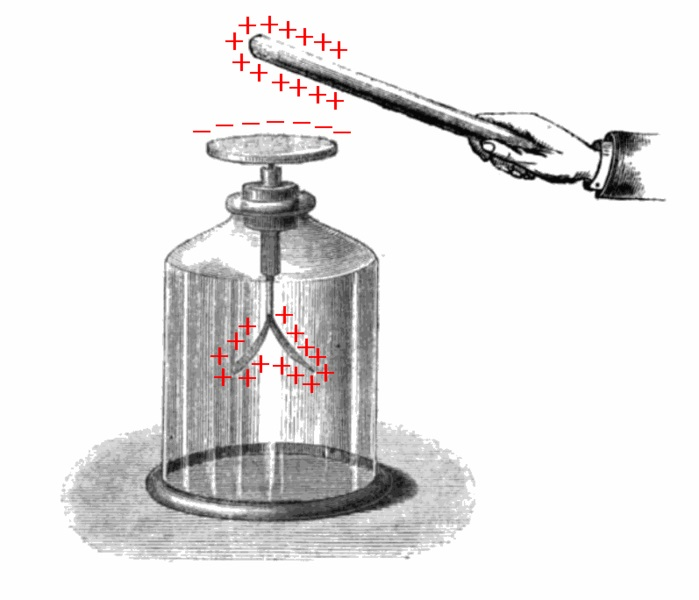
\includegraphics[width=0.4\linewidth]{images/elettroscopio}
	\caption{Schema di uno dei primi tipi di elettroscopio: quello a foglia d'oro.}
	\label{fig:elettroscopio}
\end{figure}
\FloatBarrier
L'elettroscopio (come il termoscopio) non serve per avere un valore quantitativo della carica ma permette di comparare cariche diverse, per avere un valore numerico della carica serve conoscere la legge che regola la forza elettrostatica. Tuttavia possiamo fornire una definizione operativa di due cariche uguali mediante l'elettroscopio nel modo seguente:\\
\textit{Due corpi possiedono la stessa carica se, posti a contatto con un elettroscopio scarico, generano una deflessione delle foglie di un'angolo uguale}\\
In questo modo tuttavia non si riconosce se due cariche sono dello stesso segno o meno, possiamo verificarlo semplicemente ponendo a contatto un corpo carico ad un elettroscopio scarico e poi porre il secondo a contatto con l'elettroscopio carico: se l'angolo aumenta la carica dei due corpi è uguale, se diminuisce è diversa.\\
Possiamo fare tre ulteriori riflessioni sulla carica:
\begin{itemize}
	\item La carica è quantizzata, la più piccola osservata sperimentalmente è quella dell'elettrone. Nonostante si ipotizza che i quark abbiano cariche frazionarie, queste non sono mai state osservate singolarmente
	\item La carica totale si conserva
	\item la carica non dipende dal S.I.
\end{itemize}
In queste prime sezioni tratteremo dell'elettrostatica, cioè quella branca dell'elettromagnetismo che studia sistemi all'\textbf{equilibrio elettrostatico}.
\begin{definizione}[equilibrio elettrostatico]
	L'equilibrio elettrostatico è la condizione per cui tutte le cariche presenti su di un conduttore sono ferme, è quindi assente moto di carica.
\end{definizione}
\subsection{La legge di Coulomb}
Un grande passo avanti venne fatto da Coulomb (1736-1806) che mediante esperimenti con una bilancia a torsione ottenne un metodo preciso per calcolare numericamente la forza elettrostatica e mediante al quale riuscì a ricavare l'omonima legge.\\
La bilancia di Coulomb, analoga a quella di Cavendish usata per la misura della costante di gravitazione universale, è basata sulla torsione di un filo di costante elastica c nota a causa dell'interazione elettrostatica di due corpi carichi. In particolare questa è formata da una barra sospesa mediante un filo alle estremità della quale è presente una sfera metallica ed un contrappeso, vi si avvicina un'altra carica a distanza R e si misura l'angolo a cui si dispone la prima sfera a causa della repulsione e la nuova distanza fra le due sfere. Sappiamo che il modulo del momento generato dalla torsione è
\[|\mathbf{\tau}| = c\theta\]
si ha inoltre che il momento è dato dal prodotto vettoriale delle forze applicate sulla sfera.
\[|\mathbf{\tau}| = |\mathbf{r}\wedge \mathbf{F}|\]
dove r è la distanza dall'origine al punto in cui sono applicate le forze che, per come abbiamo costruito l'apparato e scelto il sistema di riferimento ha modulo pari a metà della lunghezza della barra : L/2. 
\begin{figure}[h!]
	\centering
	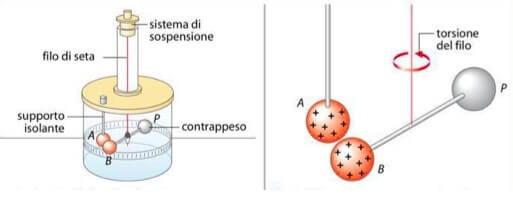
\includegraphics[width=0.6\linewidth]{images/bilancia_coulomb}
	\caption{Schemi esplicativi della bilancia di Coulomb, con cui si ottenne la legge di Coulomb.}
	\label{fig:bilanciacoulomb}
\end{figure}
\FloatBarrier
All'equilibrio le due espressioni del momento si possono eguagliare ottenendo 
\[\frac{L}{2}|\mathbf{F}|\sin\phi = c\theta\]
\[|\mathbf{F}| = \frac{2c\theta}{L\sin\phi}\] 
Possiamo trarre tre conseguenze da quanto ottenuto:
\begin{itemize}
	\item Essendo l'angolo positivo o negativo a seconda che ci sia repulsione o attrazione, $\mathbf{F}$ può avere segno negativo o positivo ed essere quindi attrattiva o repulsiva. 
	\item La forza è diretta lungo la congiungente delle cariche (versore che chiameremo $\hat{\mathbf{R}}$)
	\item A seguito di molti esperimenti si può ricavare una formula generale che è 
	\[\mathbf{F} = k \frac{q_1q_2}{r^2}\hat{\mathbf{R}}\]
	dove k è una costante da determinare, \(q_1\) e \(q_2\) sono le cariche ed r la distanza fra di esse. 
\end{itemize}
Quest'ultima è la formalizzazione della legge di Coulomb che si enuncia come segue:\\
\textit{"Date due cariche poste ad una distanza r, tra di esse si esercita una forza direttamente proporzionale al prodotto delle cariche ed inversamente proporzionale al quadrato della distanza r. Tale forza è diretta lungo la congiungente delle cariche ed è attrattiva se le cariche sono dello stesso segno e repulsiva se di segno opposto."}\\
Si noti che la forma matematica di questa legge è analoga a quella di gravitazione universale poiché entrambe le forze sono "centrali". Nella forza di Coulomb non compare il segno negativo poiché non è sempre attrattiva come quella di gravitazione ma il segno dipende dal segno delle cariche.\\
Non resta che determinare la costante k; esistono due metodi filosoficamente molto diversi fra loro:
\begin{enumerate}
	\item Nel sistema CGS  k è una grandezza adimensionale pari ad 1. Ciò discende dal fatto che in questo sistema l'unità di misura di Q è una grandezza derivata definita come
	\[[Q] = [M]^{\frac{1}{2}}[L]^{-\frac{3}{2}}[T]^{-1}\]
	Da cui deriva che K deve essere adimensionale (in realtà la definizione di Q è funzionale al definire k come adimensionale).
	\item Nel sistema MKS (che adotteremo) l'unità di misura di Q è definita come fondamentale e prende il nome di "Coulomb" (C). Sapendo la relazione che intercorre tra F e k e conoscendo l'unità di misura di F, di Q e di r possiamo ricavare l'unità di misura di k
	\[[k] = [F][L]^2[Q]^{-2} = [M][L]^3[T]^{-2}[Q]^{-1}\]
	Poniamo per convenzione (la comodità di questa scelta sarà chiara in seguito)
	\[k \equiv \frac{1}{4\pi\varepsilon_0}\]
	Da cui possiamo riscrivere la legge di Coulomb come
	\[\mathbf{F} = \frac{1}{4\pi\varepsilon_0}\frac{q_1q_2}{r^2}\hat{\mathbf{r}}\]
\end{enumerate}
Si nota sperimentalmente che la forza esercitata dalla presenza di molteplici cariche è data dalla somma vettoriale delle forze.\\
Fino al 2019 il Coulomb era definito come la forza esercitata tra due fili a distanza di un metro nei quali passa 1 Amp di corrente elettrica. Recentemente si preferisce definire le grandezze fondamentali mediante costanti di natura, il Coulomb è stato definito mediante la carica dell'elettrone: la carica dell'elettrone equivale ad una piccolissima frazione di Coulomb: 
\[e^- \equiv 1.6021766208\cdot10^{-19} C\]
Possiamo paragonare la forza di gravità a quella elettrostatica facendone il rapporto
\[\frac{F_E}{F_G} = \frac{1}{4\pi\varepsilon_0 G}\frac{|q_1||q_2|}{m_1m_2}=\simeq 2\cdot10^{39}\]
La forza elettrostatica è preponderante su quella gravitazionale tanto da renderla, in teoria, trascurabile. Tuttavia nell'esperienza quotidiana percepiamo maggiormente la gravità poiché i corpi con cui solitamente abbiamo a che fare sono neutri e in generale, a causa della repulsione di cariche dello stesso segno, è difficile che si accumulino grandi cariche, a differenza del caso di grandi masse.
\subsection{Il campo elettrostatico}
Il fatto che avvicinando due cariche esse si attraggono con una forza porta ad ipotizzare che, anche se fosse presente un'unica carica q (detta sorgente), si formerebbe comunque un \textbf{campo elettrostatico}, ovvero una regione di spazio in cui, posta una carica \(q_0\) (detta di prova), per ogni punto dello spazio si può associare ad essa un vettore forza che sperimenterebbe.\\
Matematicamente l'espressione del campo elettrostatico si ottiene semplicemente aggiungendo una parentesi nell'espressione della forza 
\[\mathbf{F}=q_0\left[\frac{1}{4\pi\varepsilon_0}\frac{q}{r^2}\hat{\mathbf{r}}\right]\]
\[\mathbf{E} = \frac{\mathbf{F}}{q_0} = \frac{1}{4\pi\varepsilon_0}\frac{q}{r^2}\hat{\mathbf{r}}\]
Si noti il salto concettuale rispetto la teoria della gravità newtoniana: ora non si tratta di trovare le forze agenti su un corpo ma il campo vettoriale, in questo caso elettrico.
\begin{definizione}[Campo elettrostatico]
	 il campo elettrico è un campo di forze generato nello spazio dalla presenza di una o più cariche elettriche. L'interazione del campo elettrostatico con una carica di prova genera una forza sulla carica stessa e, uguale e contraria, sulle cariche che generano il campo.
\end{definizione}
Un campo vettoriale può essere pensato come una porzione di spazio piena di frecce rappresentanti i vettori che esso associa ad ogni punto; disegnarlo in tal modo è impossibile dunque si opta per disegnare pochi vettori sempre tangenti al campo stesso. Per farlo si disegna un primo vettore, da esso ci si sposta di un'intervallo infinitesimo in avanti e si traccia un nuovo vettore (la cui direzione e verso saranno quelle del campo), reiterando otterremo un'insieme di vettori, se li cancelliamo e lasciamo solamente i punti di applicazione otteniamo una linea detta "di campo". Il campo elettrostatico è un vettore perché direzione e verso si ricavano dai singoli vettori mentre il modulo è dato dalla densità delle linee di campo. Per convenzione le linee di campo sono uscenti dalle cariche positive ed entranti nelle cariche negative.\\
Si osserva sperimentalmente che il campo generato da un numero discreto di cariche puntiforme è la somma vettoriale dei singoli campi, questo viene detto \textbf{principio di sovrapposizione} ed è solamente frutto dell'esperienza. Ne risulta che il campo totale generato da N cariche puntiformi è
\[\mathbf{E_{tot}} = \frac{1}{4\pi\varepsilon_0}\sum_{i=1}^{N}\frac{Q_i}{ r_i^2} \hat{\mathbf{r}}_i\]
Se invece avessimo un insieme continuo di cariche, che è ciò che avviene nella maggior parte dei casi poiché il numero di cariche è solitamente estremamente elevato, dobbiamo innanzitutto definire la densità di carica
\begin{definizione}[Densità di carica]
Definiamo la densità volumetrica di carica come
\[\rho(\mathbf{r})=\lim_{\Delta V \to 0} \frac{\Delta q}{\Delta V} = \frac{dq}{dV}\]
Definiamo analogamente la densità superficiale e lineare. 
\end{definizione}
Si noti che il limite appena scritto non ha lo stesso significato che in matematica: il volume deve essere abbastanza piccolo da racchiudere una porzione di spazio abbastanza omogenea ma non troppo piccola da mettere in luce la struttura atomica della materia.\\
Possiamo ora calcolare il campo elettrostatico generato da un corpo di carica continua 
\[\mathbf{E}_{tot} = \frac{1}{4\pi\varepsilon_0} _{\tau}\int\frac{dq}{r^2}\hat{\mathbf{r}} = \frac{1}{4\pi\varepsilon_0} _V\int\frac{\rho(\mathbf{r})}{r^2}\hat{\mathbf{r}}d\tau\]
Quest'ultimo è un integrale di volume.
\begin{esercizio}[Campo elettrostatico generato da un filo infinito carico]
Si consideri un filo di lunghezza infinita, vogliamo ottenere un'espressione del campo elettrico che genera su un punto P a distanza r' dal filo. \\
Cominciamo considerando due porzioni infinitesime di filo di lunghezza dz e carica dq, poste a distanza uguale dall'origine (uno in verso positivo ed uno in verso negativo), tracciamo i vettori $\mathbf{r}$ congiungenti le porzioni di filo con il punto P e prolunghiamo i vettori per rappresentare il campo su quel punto; $\mathbf{r}$ incide sull'asse del punto con un angolo $\theta$. Da una prima approssimazione grafica, sommando i vettori, notiamo che la componente sull'asse z si elide e il campo risultante dovrà essere parallelo all'asse delle y e in verso positivo ($\hat{\mathbf{j}}$). Possiamo quindi focalizzarci sul calcolo del modulo
\[\mathbf{E}_{tot} = _L\int dE_y\hat{\mathbf{j}}\]
\[|\mathbf{E}_{tot}| = _L\int^{+\infty}_{\infty} \frac{1}{4\pi\varepsilon_0}\frac{\lambda dz}{r^2}\cos\theta\]
le variabili \(z, \theta, r\) sono correlate quindi dobbiamo esprimere l'integrale in funzione di una sola di queste, i calcoli si semplificano se scegliamo $\theta$. r' è semplicemente la proiezione sull'asse x di r quindi si ottiene immediatamente la relazione
\[r \cos\theta = r'\]
z invece è la proiezione sull'asse y di r, per ottenere dz differenziamo
\[z = r \sin\theta = r' \tan\theta\]
\[dz = \frac{r'}{\cos^2\theta}d\theta\]
da cui l'integrale diventa
\[|\mathbf{E}_{tot}| = _L\int^{+\frac{\pi}{2}}_{-\frac{\pi}{2}} \frac{\lambda}{4\pi\varepsilon_0 r'}\cos\theta d\theta = \frac{\lambda}{2\pi\varepsilon_0 r'}\]
\end{esercizio}
La carica dell'elettrone e del protone sono esattamente uguali? Fin ora è stato visto sperimentalmente che coincidono con una precisione dell'ordine di \(10^{21}\). Se fossero diverse anche di una parte su un miliardo avremmo un effetto macrosocopico enorme: ponendo due sfere di ferro (z = 26; A = 55) a distanza di un metro, se le cariche sono esattamente uguali la forza fra esse è nulla, se invece avessimo 
\[\frac{|q_p|-|q_e|}{|q_e|} = \frac{|\Delta q|}{|q_e|}=10^{-9}\]
\[|\delta q| = |q_p|\cdot10^{-9}\]
calcoliamo la differenza di carica totale moltiplicando quella di un singolo atomo per il numero totale di atomi
\[\Delta Q = \Delta q\cdot z \left(\frac{m}{A}\cdot N_A\right) \]
\[|\mathbf{F}|=\frac{1}{4\pi\varepsilon_0}\frac{\Delta Q^2}{r^2}\simeq 1.9\cdot10^{7}\ N\]
La forza generata è enorme. 
\subsection{Potenziale elettrostatico}
Cominciamo con il chiederci se la forza elettrostatica è conservativa verificando che esiste una funzione dipendente solo dalla posizione con cui sia possibile calcolare il lavoro (il lavoro è indipendente dal percorso). 
\[L_{AB} = \int_{A}^{B}\mathbf{F}d\mathbf{l}= \frac{q_1q_2}{4\pi\varepsilon_0}\int_{A}^{B}\frac{1}{r^2}dl\cos\theta=\frac{q_1q_2}{4\pi\varepsilon_0}\int_{A}^{B}\frac{1}{r^2}dr=\frac{q_1q_2}{4\pi\varepsilon_0}\left(\frac{1}{r_A}-\frac{1}{r_B}\right)=U(B)-U(A)\]
Analogamente alla forza possiamo immediatamente verificare che il campo elettrostatico è conservativo poiché è uguale alla forza a meno di una costante
\[\int_{A}^{B}\mathbf{E}d\mathbf{l}=\frac{q}{4\pi\varepsilon_0}\left(\frac{1}{r_A}-\frac{1}{r_B}\right)=V(B)-V(A)\]
\begin{definizione}[Potenziale elettrostatico]
Definiamo la funzione di stato 
\[V(\mathbf{r}) = \frac{q}{4\pi\varepsilon_0}\frac{1}{r}\]
potenziale elettrostatico. La sua unità di misura è il Volt $V \equiv \frac{kg\cdot m^2}{s^2\cdot C}$.  Quest'ultima espressione è valida per una singola carica puntiforme. Se avessimo un numero finito di N cariche avremmo
\[V_i(\mathbf{r}) = \frac{1}{4\pi\varepsilon_0}\frac{q_i}{|\Delta \mathbf{r}_i}|\]
\[V(\mathbf{r})_i= \frac{1}{4\pi\varepsilon_0}\sum_{i}\frac{q_i}{|\Delta \mathbf{r}_i|}\]
Se avessimo una distribuzione continua di carica invece
\[V(\mathbf{r})_i= \frac{1}{4\pi\varepsilon_0}\ _Q\int\frac{d q_i}{|\Delta \mathbf{r}_i|} =  \frac{1}{4\pi\varepsilon_0}\ _V\int\frac{\rho}{|\Delta \mathbf{r}_i|}dV\]
Si ha inoltre 
\[U(\mathbf{r})=qV(\mathbf{r})\]
\end{definizione}
Le superfici equipotenziali nel caso della carica singola sono i gusci sferici concentrici centrati nella carica, il campo elettrico è sempre perpendicolare ad essi.\\
Possiamo quindi scrivere le 4 proprietà equivalenti che presenta il potenziale elettrostatico in quanto conservativo
\begin{itemize}
	\item \(\oint \mathbf{E}d\mathbf{l} = 0 \)\ per ogni percorso chiuso $\Gamma$ 
	\item \(\mathbf{\nabla}\wedge\mathbf{E} = 0\) per ogni punto
	\item \(\exists\varphi\  \text{campo scalare} : \mathbf{E}=-\mathbf{\nabla}\varphi\)=$\left(E_x = -\frac{\partial E}{\partial x},\ E_y= - \frac{\partial E}{\partial y},\ E_z= -\frac{\partial E}{\partial z}\right)$
	\item \(\varphi(B)-\varphi(A) = -\int_{A}^{B}\mathbf{\nabla}\varphi d\mathbf{l}\ \) \ per ogni percorso $\Gamma$ 
\end{itemize}
dove $\varphi = V(\mathbf{r})$.
\begin{definizione}[Forza elettromotrice (f.e.m.)]
Definiamo forza elettromotrice
\[\varepsilon \equiv \oint \mathbf{E}d\mathbf{l}\]
che è nulla per campi elettrostatici ma che può essere diversa da zero se vi sono cariche in movimento.
\end{definizione}
\begin{esercizio}[Differenza di potenziale elettrostatico di un filo infinito]
Abbiamo già calcolato il campo elettrostatico di un filo
\[\mathbf{E}(\mathbf{r}) = \frac{\lambda}{2\pi\varepsilon_0}\frac{1}{x}\hat{x}\]
Ne calcoliamo ora la differenza di potenziale elettrostatico integrando sul percorso infinitesimo \(P_0\ , P\). 
\[V(P)-V(P_0) = \int_{P_0}^{P}\mathbf{E}d\mathbf{l} = \frac{\lambda}{2\pi\varepsilon_0} \int_{P_0}^{P}\frac{dx}{x}= \frac{\lambda}{2\pi\varepsilon_0} \left(\ln(r)-\ln(r_0)\right)\]
Notiamo che il risultato ottenuto è proprio una funzione di stato dipendente solo dalla posizione più una costante arbitraria.  
\end{esercizio}
\subsection{Teorema di Gauss}
Un ulteriore metodo di calcolo del campo elettrostatico sfrutta il teorema della divergenza che, applicato al calcolo del campo elettrostatico, prende il nome di teorema di Gauss. Innanzitutto bisogna svolgere un'introduzione su angoli e angoli solidi.\\
Un'angolo è la parte di piano compresa tra due semirette aventi il vertice in comune. Sia $\hat{u}$ il versore normale all'arco di circonferenza s compreso tra le due semirette, tale da avere direzione individuata dalla retta passante dal vertice e dal centro dell'arco e verso uscente. Detto $\theta$ l'angolo ed r la distanza dal vertice al punto d'intersezione tra arco e semiretta, l'angolo è il rapporto tra l'arco di circonferenza e il raggio 
\[\theta =\frac{s}{r}\]
Considerando archi infinitesimi si ottiene
\[d\theta = \frac{ds}{r}\] 
Possiamo estendere questo concetto considerando un'ulteriore arco di circonferenza ds' compreso tra le due rette che però abbia direzione del versore diversa da $\hat{u}$, chiameremo tale nuovo versore $\hat{u'}$. I due archi si intersecano formando un angolo $\alpha$. Essendo gli archi infinitesimi possiamo considerarli come retti, otteniamo allora che ds è il cateto e ds'l'ipotenusa di un triangolo rettangolo
\[ds' \cos\alpha = ds\]
Ricordando che l'angolo è il rapporto tra arco e raggio si ottene
\[d\theta = \frac{ds'\cos\alpha}{r}\]
1 radiante per definizione è l'angolo sotteso da un arco di circonferenza che ha lunghezza pari a quella del raggio.\\
Estendiamo questo concetto in 3 dimensioni: l'angolo solido è la parte di spazio compresa tra quattro semirette. analogamente a quanto fatto con gli archi di circonferenza, possiamo individuare una calotta sferica d$\Sigma_0$ con centro nel vertice a cui associamo un versore $\hat{u}$. L'angolo solido è il rapporto fra la calotta sferica compresa tra le quattro semirette che individuano l'angolo solido e il quadrato della distanza r dei vertici della calotta dall'intersezione delle rette
\[d\Omega = \frac{\Sigma_0}{r_0^2}\]
L'unità di misura dell'angolo solido è lo steradiante, definito come l'angolo solido sotteso da una calotta sferica di superficie \(r^2\). Analogamente a quanto fatto in 2 dimensioni, consideriamo un'altra calotta sferica d$\Sigma'$ con versore diverso dal precedente e ridefiniamo lo steradiante
\[d\Omega = \frac{d\Sigma'\cos\alpha}{r^2}\] 
Consideriamo ora un angolo solido in coordinate polari come in figura 
\begin{figure}[h!]
	\centering
	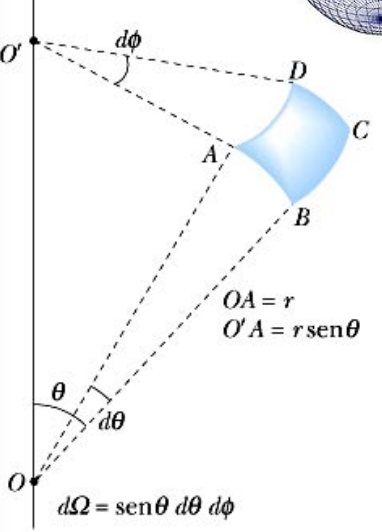
\includegraphics[width=0.5\linewidth]{images/angolo_solido}
	\caption{Schema di un angolo solido in coordinate polari}
	\label{fig:angolosolido}
\end{figure}
\FloatBarrier
Risulta, ricordando la definizione di angolo in radianti
\begin{align*}
	&d\Sigma_0 = \hat{AB}\cdot\hat{AD}\\
	&\hat{AB}=rd\theta\\
	&\hat{AD}=r\sin\theta d\varphi\\
	&d\Sigma_0 = r^2\sin\theta d\theta d\varphi\\
	&d\Omega = \frac{r^2 \sin\theta d\varphi}{r^2} = \sin\theta d\theta d\varphi
\end{align*}
Abbiamo ottenuto un'espressione dell'angolo solido in steradianti indipendente dal raggio. Per ottenere un angolo solido basta integrare su entrambe gli angoli l'angolo solido infinitesimo
\[\Omega = \int\int d\Omega = \int \int \sin\theta d\theta\]
Per integrare su tutto l'angolo solido si deve integrare \(\varphi\) da 0 a 180 e $\theta$ da 0 a 360. 
\[\Omega_{tot} = \int^{2\pi}_{0}\left(\int^{\pi}_{0} d\Omega\right)d\varphi = 2\pi \int^\pi_{0} \sin\theta d\theta = 4\pi\]
Ne segue che l'angolo solido totale è 4$\pi$, se lo moltiplichiamo per il raggio al quadrato otteniamo la superficie della sfera, proprio come moltiplicando l'angolo totale per il raggio otteniamo la circonferenza.\\\\

Vogliamo ora calcolare il flusso del campo elettrostatico: consideriamo una calotta sferica \(\sigma\) ed una sua parte infinitesima d$\mathbf{s}$, con versore normale uscente dalla parte convessa; consideriamo inoltre un vettore campo elettrostatico $\mathbf{E}$ che forma un angolo \(\theta\) con il versore $\hat{u}$. Il flusso di $\mathbf{E}$ su \(d\mathbf{s}\) è 
\[d\Phi(\mathbf{E}) = \mathbf{E}d\mathbf{s} = |\mathbf{E}||d\mathbf{s}|\cos\theta\]
Per ottenere il flusso su tutto sigma integriamo 
\[\Phi(\mathbf{E}) = \int_{\Sigma}d\Phi(\mathbf{E}) = \int_{\Sigma}\mathbf{E}d\mathbf{s} = \int_{\Sigma}|\mathbf{E}|\cos\theta|d\mathbf{s}|\]
Essendo la superficie considerata aperta, posso orientare il verso di d$\mathbf{s}$ a piacere cambiando semplicemente segno.\\
Consideriamo ora una superficie chiusa $\Sigma$ e una sua parte infinitesima $d\mathbf{s} = ds \hat{u}$, con direzione normale alla superficie e per convenzione con verso positivo quello uscente. Vogliamo calcolare il flusso elettrostatico totale della superficie chiusa; consideriamo prima l'effetto delle cariche esterne: prendiamo una carica esterna +Q e poniamola al centro di un sistema di riferimento, consideriamo un fascio di rette che stacca, intersecando la superficie chiusa, due superfici infinitesime d$\mathbf{s}_1$ e d$\mathbf{s}_2$, per le quali passa rispettivamente un campo $\mathbf{E}_1$ ed $\mathbf{E}_2$ (su ogni punto della superficie chiusa esiste campo elettrostatico generato dalla carica).  
\begin{figure}[h!]
	\centering
	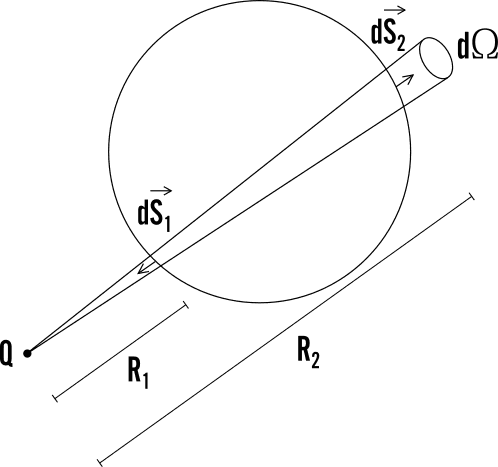
\includegraphics[width=0.5\linewidth]{images/thm_gauss_1}
	\caption{Schema del fascio di rette che partono da una carica esterna e staccano due superfici infinitesime dalla superficie chiusa}
	\label{fig:thmgauss1}
\end{figure}
\FloatBarrier
Si noti che l'angolo che forma il campo elettrico con la superficie infinitesima è rispettivamente \(\theta_1\) e \(\theta_2\); essendo la direzione del campo generata da una carica costante nello spazio, si ha
\[\theta_1 = \theta_2 + 180\]
\[\Rightarrow \cos\theta_1 = -\cos\theta_2\]
Possiamo calcolare il flusso delle due superfici infinitesime, ricordando la definizione di steradiante precedentemente ottenuta
\begin{align*}
	&d\Phi_2 = \mathbf{E}_2\cdot d\mathbf{s}_2 = |\mathbf{E}_2| ds_2 \cos\theta_2 = |\mathbf{E}_2| R_2^2 \frac{ ds_2 \cos\theta_2}{R_2^2} = |\mathbf{E}_2| R_2^2 d\Omega_2 =\frac{1}{4\pi\varepsilon_0}\frac{Q}{R^2_2}R^2_2= \frac{Q}{4\pi\varepsilon_0}d\Omega \\
	&d\Phi_1 = \mathbf{E}_1\cdot d\mathbf{s}_1 = |\mathbf{E}_1| ds_1 \cos\theta_1 = -|\mathbf{E}_1| ds_1 \cos\theta_2 = -\frac{Q}{4\pi\varepsilon_0}d\Omega\\
	&\Rightarrow d\Phi_{12} = d\Phi_1 + d\Phi_2 = 0
\end{align*}
Non avendo usato specifiche proprietà della carica esterna o del campo o della superficie chiusa considerata possiamo dedurre che il flusso per una superficie chiusa di ogni carica esterna è nullo; per calcolare il flusso basta considerare quelle interne.\\
Consideriamo quindi una superficie \(\Sigma\) con una carica +Q al suo interno che sta al centro del nostro sistema di riferimento, consideriamo una superficie infinitesima d$\mathbf{s}$ a distanza r da Q, l'angolo fra d$\mathbf{s}$ ed $\mathbf{E}$ sarà $\theta$. Si noti che, essendo la carica positiva per ipotesi, il flusso è positivo per ogni punto della superficie mentre per una carica esterna poteva essere o positivo o negativo. Calcoliamo quindi il flusso
\begin{align*}
	&d\Phi(\mathbf{E}) = \frac{Q}{4\pi\varepsilon_0}d\Omega\\
	&\Phi(\mathbf{E}) = \oint_{\Sigma} d\Phi(\mathbf{E}) = \frac{Q}{4\pi\varepsilon_0}\oint_0^{4\pi}d\Omega = \frac{Q}{\varepsilon_0} = \int_{V(\Sigma)}\frac{\rho}{\varepsilon_0}d\tau
	\end{align*}
dove l'ultimo è un'integrale su tutto il volume racchiuso dalla superficie $\Sigma$ della densità volumetrica di carica e $\tau$ è una porzione di volume infinitesima. Questo risultato, in virtù del principio di sovrapposizione, vale anche per N cariche, dove al posto del singolo Q avremo la somma algebrica delle cariche 
\[Q_{tot} = \sum_iq_i\ \text{caso discreto}\]. 
\[Q_{tot} = \int_{V(\Sigma)}\rho d\tau\ \text{caso continuo}\]
Possiamo quindi enunciare il \textbf{teorema di Gauss}:\textit{Il flusso del campo elettrostatico attraverso una qualsiasi superficie chiusa $\Sigma$ è pari alla somma algebrica delle cariche in \(\Sigma\) diviso la costante dielettrica del vuoto $\varepsilon_0$.}
Riassumendo, la forma integrale del teorema di Gauss è:
\[\oint\mathbf{E}d\mathbf{s} = \frac{Q_{tot}}{\varepsilon_0}\]
Si noti che la legge di Gauss è valida in virtù del fatto che, per la legge di Coulomb, il campo elettrostatico diminuisce quadraticamente con la distanza ma anche la superficie che stacca l'angolo solido aumenta quadraticamente con la distanza quindi le due si compensano e ne risulta che il flusso non dipende dalla distanza.\\
Si noti inoltre che la legge di Gauss espressa in questa forma (integrale) esprime una proprietà media della superficie chiusa $\Sigma$. Possiamo esprimere la stessa legge in forma differenziale confrontando il teorema della divergenza (\ref{ap:thm_divergenza}) con quello di Gauss
\begin{align*}
	&\text{Thm. di Gauss: }\ \oint\mathbf{E}d\mathbf{s} = \int_{V(\Sigma)}\rho d\tau\\
	&\text{Thm. della divergenza: }\ \oint\mathbf{E}d\mathbf{s} = \int_{V(\Sigma)}\mathbf{\nabla}\cdot\mathbf{E}\ d\tau \\
	&\Rightarrow \mathbf{\nabla}\cdot\mathbf{E} = \frac{\rho}{\varepsilon_0}
\end{align*} 
Il teorema di Gauss in forma differenziale esprime una proprietà puntuale del flusso sulla superficie $\Sigma$. Si noti, ad esempio, nella forma differenziale si nota immediatamente che la divergenza del campo elettrico in un punto senza carica è nulla poiché la densità di carica in quel punto è nulla. Possiamo anche verificarlo calcolando la divergenza
\begin{align*}
	&\mathbf{E} = \frac{Q}{4\pi\varepsilon_0}\frac{\mathbf{r}}{|\mathbf{r}|^3} = \frac{Q}{4\pi\varepsilon_0}\frac{x\hat{\mathbf{i}}+y\hat{\mathbf{j}}+z\hat{\mathbf{k}}}{(x^2+y^2+z^2)^{\frac{3}{2}}}\\
	&\mathbf{\nabla}\cdot\mathbf{E} = \frac{Q}{4\pi\varepsilon_0}\left(\frac{\partial}{\partial x}\frac{x}{(x^2+y^2+z^2)^{\frac{3}{2}}}+\frac{\partial}{\partial y}\frac{y}{(x^2+y^2+z^2)^{\frac{3}{2}}}+\frac{\partial}{\partial z}\frac{z}{(x^2+y^2+z^2)^{\frac{3}{2}}}\right)=\\
	& \frac{Q}{4\pi\varepsilon_0}\left(\frac{1}{(x^2+y^2+z^2)^{\frac{5}{2}}}\right)(-2x^2+y^2+z^2+x^2-2y^2+z^2+x^2+yì2-2z^2) = 0
\end{align*}
Infine, riproponiamo gli esercizi del calcolo del campo elettrostatico generato da un filo e da un piano su un punto a distanza r, già risolti in due modi differenti in precedenza
\begin{esercizio}[Campo elettrostatico generato da un filo infinito carico]
Sia $\lambda$ la densità di carica lineare del filo. Si noti che sussiste una simmetria cilindrica nel campo elettrostatico generato dal filo: consideriamo una superficie cilindrica di raggio di base r uguale alla distanza di P dal filo e di altezza h. Per il teorema di Gauss sappiamo che
\[\oint_{\Sigma}\mathbf{E}d\mathbf{s}=\frac{Q_{tot}}{\varepsilon_0} = h\lambda\]
Possiamo parimenti calcolare il flusso dividendo l'integrale chiuso in 3 integrali aperti: due per le basi ed uno per la superficie laterae del cilindro. Notiamo immediatamente che l'angolo formato fra la normale alla superficie delle basi e il campo elettrostatico è di 90 gradi, ne segue che il prodotto scalare è nullo e il flusso sulle due facce di base è nullo. Consideriamo ora il flusso sulla superficie laterale, campo elettrostatico e vettore superficie sono paralleli in ogni punto: l'angolo formato è sempre nullo e il coseno è sempre 1.
\[\oint_{\Sigma}\mathbf{E}d\mathbf{s}=\int_{\Sigma_l}\mathbf{E}d\mathbf{s}_l= \int_{\Sigma_l}|\mathbf{E}|d\mathbf{s}_l|\]
Ricordiamo infine che sulla superficie laterale il campo è costante quindi lo portiamo fuori dall'integrale
\[\oint_{\Sigma}\mathbf{E}d\mathbf{s}=|\mathbf{E}|\int_{\Sigma_l}ds_l=|\mathbf{E}|2\pi r h\]
Infine, eguagliando le due espressioni ottenute
\[|\mathbf{E}|= \frac{\lambda}{\varepsilon_0 2\pi r }\]
\end{esercizio}
\begin{esercizio}[Campo elettrostatico generato da un piano infinito carico]\label{es:campo_piano_infinito}
Sia $\sigma$ la densità di carica superficiale del piano. Notiamo che tutti i piani paralleli al piano carico presentano medesimo campo elettrostatico in ogni punto. Consideriamo il cilindro "coricato" con basi parallele al piano carico, altezza 2r (il piano taglia in due parti uguali il cilindro) e il punto P al centro del cerchio che sta alla base del cilindro. Analogamente a quanto fatto precedentemente, per il teorema di Gauss abbiamo:
\[\oint\mathbf{E}d\mathbf{s} = \frac{Q_{tot}}{\varepsilon_0}=\frac{\sigma}{\varepsilon_0}\int_Sds=\frac{A\sigma}{\varepsilon_0}\]
dove A è l'area di base del cilindro.\\
Ricalcoliamo ora il flusso dividendo l'integrale nelle tre superfici: sulla superficie laterale il vettore superficie è sempre perpendicolare a quello del campo elettrostatico quindi il flusso è nullo. Sulle due facce di base invece l'angolo è zero, inoltre essendo in entrambe i casi flusso uscente bisognerà sommare i due flussi
  \[\oint\mathbf{E}d\mathbf{s} = 2\int_{\Sigma_b}\mathbf{E}d\mathbf{s}_b= 2A|\mathbf{E}|\]
Eguagliando le due espressioni ottenute si perviene a 
\[|\mathbf{E}|=\frac{\sigma}{2\varepsilon_0}\]
Il campo ha direzione opposta dai due lati della superficie, la discontinuità che si osserva attraversando la superficie da un lato all'altro è dunque di
\[E_1-E_2 = \frac{\sigma}{2\varepsilon_0}-\left(-\frac{\sigma}{2\varepsilon_0}\right) = \frac{\sigma}{\varepsilon_0}\]
Si noti infine che nel caso del piano carico il flusso non dipende dalla distanza del punto poiché, essendo il piano infinito, aumentare la distanza porterebbe solo a "riscalare" il tutto ottenendo lo stesso flusso.
\end{esercizio}
\subsubsection{Discontinuità del campo elttrico attraverso una superficie carica}
Osserviamo ora delle proprietà interessanti del campo elettrostatico, quando si attraversa una superficie carica.\\
Consideriamo una superficie generica (non omogenea), costruiamo un cilindro che la interseca, visto che ci interessa sapere cosa accade nel passaggio da una faccia all'altra della superficie consideriamo un cilindro con altezza \(dh\to 0\), da ciò deriva che la componente di flusso per la superficie laterale del cilindro non è rilevante. Il flusso è quindi
\[\oint_{\Sigma}\mathbf{E}d\mathbf{s} = \mathbf{E}_{u}d\mathbf{s}_{u}+\mathbf{E}_{d}d\mathbf{s}_d=(E_u\cos\theta_u-E_d\cos\theta_d)dA = dA(E_{\perp u}-E_{\perp d})\] 
Per il teorema di Gauss, essendo la superficie del cilindro chiusa e $\sigma$ la densità di carica superficiale, si ha
\[\oint_{\Sigma}\mathbf{E}d\mathbf{s} = \frac{Q_{tot}}{\varepsilon_0} = \frac{\sigma dA}{\varepsilon_0}\] 
\[\Rightarrow |\Delta \mathbf{E}_{\perp}| = (E_{\perp u} - E_{\perp d}) = \frac{\sigma}{\varepsilon_0}\]
Ne segue che la discontinuità della componente perpendicolare alla superficie, nell'attraversarla, presenta un salto pari a \(\frac{\sigma}{\varepsilon_0}\) (non si hanno informazioni su come sia distribuita questa quantità fra le due facce). Si noti che è la stessa discontinuità ottenuta nell'esercizio (\ref{es:campo_piano_infinito}).\\
Ci chiediamo ora cosa accada alla componente tangente al campo nell'attraversare una superficie carica. Per farlo consideriamo la circuitazione del campo elettrostatico, calcolandola in un percorso rettangolare che interseca la superficie perpendicolarmente, a metà dei due lati perpendicolari. Essendo il campo conservativo abbiamo che la circuitazione deve essere nulla
\[\oint_\Gamma\mathbf{E}d\mathbf{r} = 0\]
D'altro canto possiamo calcolare la circuitazione lato per lato; visto che ci interessa il passaggio fra le due facce consideriamo un percorso rettangolare la cui altezza tenda a zero \(dh\to 0\) (considereremo solo i lati orizzontali del circuito).  
\[\oint_\Gamma \mathbf{E}d\mathbf{r} = \mathbf{E}_1 d\mathbf{l}_1 + \mathbf{E}_3d\mathbf{l}_3 = E_1dl_1\cos\theta_1 + E_3dl_3\cos\theta_3 = (E_{T1}-E_{T3})dl\]
Dove la t al pedice indica la componente tangenziale. Eguagliando le due espressioni ottenute si ha
\[\Rightarrow E_{T1}=E_{T3}\]
Ne segue quindi che la componente tangenziale resta continua attraversando la superficie. 
\section{Elettrostatica della materia: i conduttori}
\subsection{Conduttori neutri}
I materiali si suddividono nelle due macrocategorie di conduttori e dielettrici (isolanti). Un conduttore metallico come il rame può essere modellizzato, in prima approssimazione, come un reticolo di ioni vincolati fra loro che possono solamente vibrare, immersi in un mare di elettroni tanto debolmente legati al nucleo da poter muoversi liberamente attorno al reticolo a seguito di eccitazioni energetiche minime come 'agitazione termica. Ogni atomo di rame contribuisce con circa un elettrone di conduzione, in un centimetro cubo vi sono
\[n_e = \frac{\rho_M }{A}N_A \simeq 8\cdot 10^22\ \frac{e^-}{cm^3}\simeq13000\ \frac{C}{cm^3}\]
dove $\rho_M$ è la densità ed A è la massa molare.
\begin{definizione}[Conduttore elettrico]
	Un conduttore elettrico è un materiale in grado di far scorrere corrente elettrica al suo interno. I materiali conduttori sono caratterizzati dalla presenza di elettroni liberi nella banda di valenza degli atomi del reticolo cristallino (conduttori di prima specie) o contengono specie ioniche che si fanno carico di trasportare la corrente (conduttori di seconda specie).
\end{definizione}
Di seguito elenchiamo, dimostrandole, 6 proprietà dei conduttori:
\begin{enumerate}
\item	Se inserisco un conduttore in un campo elettrico uniforme, ogni elettrone sperimenta una forza di verso opposto a quello del campo elettrostatico
\[\mathbf{F} = -e\mathbf{E} = m_e \mathbf{a}\]
Se aspettiamo un tempo sufficientemente lungo gli elettroni si sposteranno ed il sistema sarà nuovamente all'equilibrio (è un fatto sperimentale che a un certo punto gli elettroni smettono di muoversi). Se gli elettroni smettono di muoversi (intendendo movimento in media) vuol dire che una forza si oppone a quella generata dal campo elettrostatico, quale? Quando gli elettroni si spostano tutti nello stesso verso si crea una zona a prevalenza di cariche positive (il reticolo di ioni privo di elettroni) che attrae per forza di Coulomb gli elettroni a sè opponendosi alla forza generata dal campo elettrostatico. Passando da termini di forza a termini di campo, potremo dire che all'interno del conduttore si è creato un \textbf{campo elettrostatico indotto}, opposto a quello esterno (in verso e modulo). Abbiamo quindi che il campo elettrostatico totale all'interno di un conduttore è
\[\mathbf{E}_{tot} = \mathbf{E}_I+\mathbf{E}_E = 0\]
\textit{Il campo elettrico totale all'equilibrio, all'interno di un conduttore, è nullo, anche in presenza di un campo elettrostatico esterno}.
\item Possiamo applicare la legge di Gauss al caso appena visto 
\[\oint_{\Sigma}\mathbf{E}_{tot}d\mathbf{s}= \frac{Q_{tot}}{\varepsilon_0} = 0\]
\[\Rightarrow Q_{tot} = 0\]
Possiamo svolgere lo stesso ragionamento puntualmente usando la forma differenziale del teorema di Gauss
\[\mathbf{\nabla}\mathbf{E}_{tot}=\frac{\rho}{\varepsilon_0}=0 \]
\[\Rightarrow \rho = 0,\ \forall P \in C\]
dove C è l'insieme di punti all'interno del conduttore. \\
\textit{All'interno di un conduttore, in ogni punto, la densità di carica elettrica è nulla. In totale, all'interno del conduttore la carica totale è nulla. Ci sono quindi tante cariche positive quante negative. Il conduttore resta neutro prima e dopo l'applicazione di un campo elettrostatico $\mathbf{E}$}.
\item Essendo la densità di carica nulla all'interno di tutto il conduttore, è intuitivo pensare che le cariche si dispongano sulla superficie; a riprova di ciò ricordiamo che abbiamo già ottenuto che la componente normale di campo elettrico alla superficie di un piano carico presenta una discontinuità proprio sulla superficie di \(\frac{\sigma}{\varepsilon_0}\) da cui segue che la densità di carica non è nulla sulla superficie. \\
\textit{Le cariche di un conduttore immerso in un campo elettrostatico si dispongono sulla superficie}.
\item Osserviamo che le linee di campo non possono essere tangenti rispetto la superficie del conduttore perché sappiamo che queste devono essere continue prima e dopo la superficie e sappiamo anche che all'interno il campo è nullo. Per le stesse considerazioni non può esistere una componente tangente quindi saranno sicuramente ortogonali. Non può essere ortogonale verso l'interno perché altrimenti sposterebbe le cariche verso l'interno generando campo elettrostatico all'interno del conduttore ma sappiamo che in questa regione il campo è nullo. Ne segue che le linee di campo sono ortogonali dirette perso l'esterno (se la carica è positiva, se negativa si cambia il segno).\\
\textit{L'immersione di un conduttore in un campo elettrostatico provoca un'alterazione del campo preesistente sia all'interno del conduttore (si annulla) sia all'esterno (si piega per entrare ed uscire perpendicolarmente alla superficie del conduttore)}.
\item Studiamo il potenziale elettrostatico sulla superficie del conduttore: consideriamo i punti A, B e calcoliamone il potenziale
\[\Delta V_{AB} = V_B - V_A = \int_A^B \mathbf{E}d\mathbf{r} = 0\]
\'E nullo perché d$\mathbf{r}$ è tangente alla superficie per definizione mentre il campo è ortogonale ad essa, il prodotto scalare è dunque identicamente nullo. Inoltre, essendo il campo nullo all'interno del conduttore, presi due punti qualsiasi in questa regione, il potenziale è sempre nullo e quindi sempre uguale.\\
\textit{La superficie di un conduttore è equipotenziale come i punti al suo interno}.
\item Consideriamo ora un conduttore cavo, possiamo individuare una superficie esterna $\Sigma_E$, su cui sappiamo sono disposte le cariche, ed una superficie interna $\Sigma_I$, ci chiediamo come sono disposte le cariche su questa superficie. Consideriamo una generica superficie $\Sigma$ compresa tra quella interna e quella esterna, applichiamo la legge di Gauss
\[\oint_\Sigma \mathbf{E}d\mathbf{s} = \frac{Q_{tot}}{\varepsilon_0} = 0 \Rightarrow Q_{tot} = 0\]
La carica totale all'interno di questa superficie è nulla, essendo $\Sigma$ arbitraria possiamo prenderla infinitamente vicina a $\Sigma_I$ ottenendo che l'unica disposizione possibile sarebbe con le cariche positive e negative sono in numero eguale e disposte sula superficie interna come su quella esterna (metà da una parte e metà dall'altra a bilanciarsi). Tuttavia in questo caso si violerebbe la conservatività del campo elettrostatico: consideriamo un percorso chiuso passante in parte dall'interno cavo (AB) ed in parte tra $\Sigma_I$ e $\Sigma_E$, avremmo
\[\oint_{\Gamma}\mathbf{E}d\mathbf{r}= \int_{A}^{B}\mathbf{E}d\mathbf{r}+\int_{B}^{A}\mathbf{E}d\mathbf{r}\]
Il secondo addendo è nullo perché abbiamo visto che all'interno del conduttore il campo è identicamente nullo mentre il primo addendo è diverso da zero perché d$\mathbf{r}$ è parallelo a $\mathbf{E}$. Ne segue che la circuitazione non è nulla e la conservatività del campo è violata, il che è assurdo. ne segue per esclusione che non vi sono cariche sulla superficie interna del conduttore cavo. Ciò spiega perché all'interno di un ascensore (metallico) il telefono non prende (no campo). 
\textit{Se ho un conduttore cavo la redistribuzione delle cariche riguarda solo la superficie esterna}. 
\end{enumerate}
\begin{esercizio}[Campo elettrostatico di un cilindro carico di altezza infinita]
Consideriamo un cilindro carico con densità volumetrica di carica uniforme $\rho$, raggio di base R e altezza h infinita. Cominciamo calcolando il campo all'esterno del cilindro circondandolo con una superficie cilindrica di raggio \(r>R\). Per il teorema di Gauss abbiamo
\[\oint_{\Sigma}\mathbf{E}d\mathbf{s}=\frac{Q_{tot}}{\varepsilon_0}\]
Calcolando invece il flusso dividendo la superficie cilindrica in tre superfici (area laterale e due basi) notiamo che il flusso per le masi è nullo, inoltre il campo sulla superficie laterale è costante data la simmetria cilindrica dell'oggetto carico considerato.
\[\oint_{\Sigma}\mathbf{E}d\mathbf{s}=\int E ds_l = E\int ds = E2\pi r h\]
Considerato che
\[Q_{tot} = \rho V = \rho \pi R^2 h\]
si ottiene
\[\mathbf{E}_{est} = E \hat{\mathbf{i}} = \frac{\rho \pi R^2 h }{2\pi r h \varepsilon_0} \hat{\mathbf{i}}= \frac{\rho R^2 }{2 r \varepsilon_0}\hat{\mathbf{i}}\]
\end{esercizio}
Ora calcoliamo il campo all'interno del cilindro, analogamente a prima consideriamo una superficie cilindrica questa volta interna al cilindro carico (\(r<R\)). 
\[\oint_{\Sigma}\mathbf{E}d\mathbf{s}=\frac{Q_{tot}}{\varepsilon_0} = \frac{\rho 2 \pi r^2}{\varepsilon_0}\]
\[\oint_{\Sigma}\mathbf{E}d\mathbf{s}=E\int ds_l = E2\pi rh\]
\[\mathbf{E}_{int} = \frac{\rho r}{2\varepsilon_0}\hat{\mathbf{i}}\]
Possiamo ottenere il valore del campo sulla superficie usando una delle due relazioni ottenute sostituendo R = r
\[\mathbf{E}_{sup} = \frac{\rho R}{2\varepsilon_0}\hat{\mathbf{i}}\]
Infine la differenza di potenziale fra due punti a distanza \(r_1\) ed \(r_2\) è
\[V(r_2)-V(r_1) = \int_{r_1}^{r_2}\mathbf{E}d\mathbf{r}=\ln\left(\frac{r_2}{r_1}\right)\frac{\rho R^2}{2\varepsilon_0}\]
\begin{esercizio}[Campo elettrostatico di un guscio sferico carico]
Consideriamo un guscio sferico di raggio R e densità superficiale di carica $\sigma$. Per ottenere il campo all'esterno del guscio uguagliamo la legge di Gauss al calcolo del flusso integrando sulla superficie, la direzione del campo sappiamo essere sempre perpendicolare alla superficie della sfera quindi avrà versore $\hat{\mathbf{r}}$.
\[\oint_{\Sigma}\mathbf{E}_{est}d\mathbf{s} = \frac{Q_{tot}}{\varepsilon_0} = \frac{4\pi R^2 \sigma}{\varepsilon_0}\]
Per il calcolo del flusso consideriamo una superficie sferica esterna di raggio \(r>R\)
\[\oint_{\Sigma}\mathbf{E}_{est}d\mathbf{s} = E\oint ds = E_{est} 4\pi r^2\]
\[\Rightarrow \mathbf{E}_{est} = \frac{R^2 \sigma}{r^2 \varepsilon_0} \hat{\mathbf{r}}\]
Per ottenere il campo all'interno del guscio notiamo che applicando il teorema di Gauss considerando una superficie sferica \(r<R\) abbiamo che \(Q_{tot}\) interna è nulla quindi anche il campo elettrostatico lo è. Abbiamo quindi una discontinuità di $\frac{\sigma}{\varepsilon_0}$ sulla superficie proprio come dimostrato in precedenza. Infatti per calcolare il campo sulla superficie è sufficiente porre \(r=R\) nella formula per il campo esterno.\\
Per il potenziale basta integrare il campo in d$\mathbf{r}$ ottenendo
\[V(r)_{est} = \int_{r}^{+\infty} \frac{R^2 \sigma}{r^2 \varepsilon_0} dr = \frac{R^2 \sigma}{ r\varepsilon_0}\]
\[V(r)_{int} = \int^{R}_r 0 dr = costante \]
Dove la costante si ricava osservando che il potenziale è funzione continua di r quindi deve assumere lo stesso valore da r ad R; possiamo calcolarne il valore in R usando la formula per il campo esterno
\[V(r)_{int} = \frac{R \sigma}{\varepsilon_0}\]
\end{esercizio}
\begin{esercizio}[Campo elettrostatico di una sfera piena carica]
Consideriamo ora una sfera piena carica di raggio R e densità volumetrica di carica $\rho$ (la carica è distribuita uniformemente sul volume). Per il campo esterno consideriamo una superficie sferica di raggio \(r>R\), eguagliando legge di Gauss e calcolo del flusso otteniamo analogamente a prima 
\[\mathbf{E}_{est} = \frac{\rho R^3}{3 \varepsilon_0 r^2}\hat{\mathbf{r}}\]
All'interno invece consideriamo una sfera di raggio \(r<R\), ora nella legge di Gauss la carica totale non sarà quella di tutta la sfera carica ma solamente quella all'interno della superficie sferica considerata. 
\[\oint_{\Sigma}\mathbf{E}d\mathbf{s}=\frac{Q_{tot}}{\varepsilon_0} = \frac{\rho 4 \pi r^3}{3\varepsilon_0}\]
\[\oint_{\Sigma}\mathbf{E}d\mathbf{s}=E\int ds = E 4\pi r^2\]
\[\Rightarrow \mathbf{E}_{int} = \frac{\rho r}{3 \varepsilon_0}\hat{\mathbf{r}}\]
Dunque la carica all'interno cresce linearmente con la distanza dal centro della sfera fino alla superficie (dove arriva al valore di \(\frac{\rho R}{3 \varepsilon_0}\)) per poi decrescere quadraticamente con la distanza dal centro della sfera.\\
Per il potenziale basta integrare il campo in d$\mathbf{r}$ ottenendo
\[V(r)_{est} = \int_{r}^{+\infty} \frac{\rho R^3}{3 \varepsilon_0 r^2}dr = \frac{\rho R^3}{3 \varepsilon_0 r}\]
Dunque sulla superficie della sfera abbiamo
\[V(R) = \frac{\rho R^2}{3 \varepsilon_0 }\]
\[V(r)_{int} = \int_{r}^{+\infty} \frac{\rho r}{3 \varepsilon_0} dr = \int_{r}^{R}\frac{\rho r}{3 \varepsilon_0} dr+\int_{R}^{+\infty}\frac{\rho r}{3 \varepsilon_0} dr =\frac{\rho}{6\varepsilon_0}\left(R^2-r^2\right) +\frac{\rho R^2}{3 \varepsilon_0 }\]
\end{esercizio}
\begin{esercizio}[Campo elettrostatico di un anello carico]
Consideriamo un anello carico di densità lineare di carica $\lambda$, carica totale Q e raggio R ed un punto P a distanza R dal centro dell'anello come in figura.
\begin{figure}[h!]
	\centering
	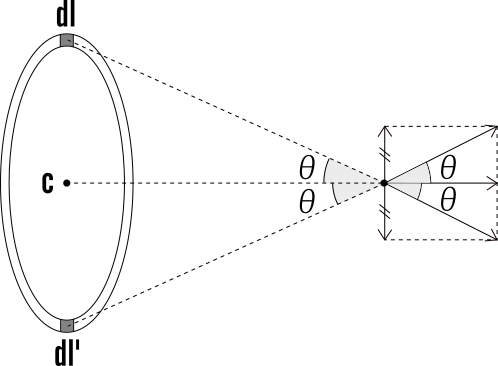
\includegraphics[width=0.6\linewidth]{images/anello}
	\caption{Schema per il calcolo del campo elettrico di un anello carico}
	\label{fig:anello}
\end{figure}
\FloatBarrier
Per il principio di sovrapposizione risulta che il campo risultante giace solo sull'asse z. Calcoliamo il campo elettrico generato da una porzione dl dell'anello, a distanza z dal punto P
\[dq = dl\lambda = R d\alpha \lambda\] 
\[d\mathbf{E} = \frac{ R d\alpha\lambda \cos\theta}{4\pi\varepsilon_0z^2}\hat{\mathbf{k}} = \]
Notiamo che $\cos\theta = \frac{r}{z}$
\[d\mathbf{E} = \frac{ R d\alpha\lambda r }{4\pi\varepsilon_0 z^3}\hat{\mathbf{k}} = \frac{ R d\alpha\lambda r }{4\pi\varepsilon_0 (R^2+r^2)^{\frac{3}{2}}}\hat{\mathbf{k}}\]
Per ottenere il campo totale integriamo 
\[\mathbf{E} = \frac{ R \lambda r }{4\pi\varepsilon_0 (R^2+r^2)^{\frac{3}{2}}}\hat{\mathbf{k}}\int_{0}^{2\pi}d\alpha= \frac{ R \lambda r }{2\varepsilon_0 (R^2+r^2)^{\frac{3}{2}}}\hat{\mathbf{k}} \]
Per ottenere il potenziale integriamo il campo in dr
\[V(r) = \frac{R \lambda}{2\varepsilon_0}\int_{r}^{+\infty}\frac{  r }{ (R^2+r^2)^{\frac{3}{2}}} dr= \frac{R \lambda}{2\varepsilon_0}\frac{1}{2}\int_{r}^{+\infty}\frac{ dx }{ x^{\frac{3}{2}}} = \frac{ R \lambda }{2\varepsilon_0 (R^2+r^2)^{\frac{1}{2}}}\]
dove nell'ultimo passaggio è stato sostituito \(R^2+r^2 = x\).
\end{esercizio}
\begin{esercizio}[Campo elettrostatico di un disco carico]
Ora, al posto di un anello consideriamo un disco di densità superficiale di carica $\sigma$ e raggio R. Possiamo sfruttare il campo dell'anello appena ottenuto ed integrarlo da 0 ad R. per farlo esprimiamo la carica infinitesima come la carica contenuta in un anello si spessore infinitesimo
\[dq = \sigma 2\pi l dl\]
dove l è stato sostituito al precedente R perché quest'ultimo era costante mentre l dovrà essere la nostra variabile di integrazione. 
\[d\mathbf{E} = \frac{  \sigma l dl r }{2\varepsilon_0 (l^2+r^2)^{\frac{3}{2}}}\hat{\mathbf{k}}\]
\[\mathbf{E} = \frac{\sigma r}{2\varepsilon_0}\int_{0}^{R}\frac{ldl}{(l^2+r^2)^{\frac{3}{2}}} = \frac{\sigma r}{2\varepsilon_0}\left[-\frac{1}{(l^2+r^2)^{\frac{1}{2}}}\right]^R_0 = \frac{\sigma }{2\varepsilon_0}\left[\frac{r}{|r|}-\frac{r}{\sqrt{R^2+r^2}}\right]\]
Si noti che il valore assoluto porta una discontinuità tale che per \(z\to0^+\) si ha \(E = \frac{\sigma}{2\varepsilon_0}\) e per \(z\to0^-\) si ha \(E = -\frac{\sigma}{2\varepsilon_0}\); la discontinuità nell'attraversare la superficie del disco è quindi \(\frac{\sigma}{\varepsilon_0}\) come dimostrato nel caso generale in precedenza.
\end{esercizio}
\begin{esercizio}[Campo elettrostatico di uno spessore di carica di superficie infinita]
Consideriamo una lastra carica di superficie infinita spessa D di densità di carica volumetrica uniforme $\rho$. Consideriamo un cilindro di asse perpendicolare al piano della lastra di basi \(B_1\) e \(B_2\), eguagliamo la legge di Gauss al calcolo del flusso (che sulla superficie laterale del cilindro è nullo) per ottenere il campo all'esterno della lastra. 
\[\Phi(\mathbf{E}) = \frac{Q_{tot}}{\varepsilon_0} = \frac{\rho A D}{\varepsilon_0}\]
\[\Phi(\mathbf{E}) = 2EA\]
\begin{align*}
	\mathbf{E} =
	\begin{cases}
	\frac{\rho D}{2\varepsilon_0}\hat{\mathbf{k}}\ se\ x>D/2\\
	-\frac{\rho D}{2\varepsilon_0}\hat{\mathbf{k}}\ se\ x<D/2\\
	\end{cases}
\end{align*}
 Per il calcolo del campo all'interno (\(-D/2<x<D/2\)), il flusso calcolato con l'integrale di superficie resta lo stesso mentre quello calcolato con Gauss diventa
  \[\Phi(\mathbf{E}) = \frac{Q_{tot}}{\varepsilon_0} = \frac{\rho A 2x}{\varepsilon_0} \]
  \[\Rightarrow \mathbf{E} = \frac{\rho x}{\varepsilon_0}\hat{\mathbf{k}}\]
\end{esercizio}
Analizziamo infine l'ultima casistica riguardante i conduttori neutri: un conduttore cavo con una carica +Q all'interno della cavità. La carica genera un campo le cui linee entrano perpendicolarmente sulla superficie intera del conduttore. Consideriamo una superficie $\Sigma'$ intermedia tra le superfici interna ed esterna del conduttore, abbiamo già dimostrato che il flusso all'interno di $\Sigma'$ è nullo poiché una superficie all'interno del conduttore, per annullare il campo generato dalla carica +Q, dovrà disporsi sulla superficie interna una carica -Q, per controbilanciare il campo. Essendo il conduttore neutro, all'esterno di $\Sigma'$ dovrà esserci una carica +Q, che genera un campo elettrico all'esterno del conduttore. Questo, per la legge di Gauss applicata ad una superficie esterna al conduttore $\Sigma''$, ha intensità $\frac{Q}{\varepsilon_0}$. Questo fenomeno, per cui tutte le linee di campo interne al conduttore escono da esso, viene detto \textbf{induzione completa}.  
\subsection{Conduttori carichi}
Generalizziamo ora quanto ottenuto per conduttori neutri a conduttori carichi. Euristicamente, le cariche essendo dello stesso segno si respingono e si dispongono a distanza massima fra di esse : sulla superficie. Questo fenomeno è del tutto simile a quello dell'induzione quindi possiamo enunciare le stesse proprietà da essa derivanti
\begin{enumerate}
	\item Dentro il conduttore il campo è nullo.
	\item La densità di carica è nulla quindi le cariche si dispongono sulla superficie.
	\item Il campo è normale alla superficie e la discontinuità del modulo della componente perpendicolare del campo è $\frac{\sigma}{\varepsilon_0}$.
	\item Ogni punto interno al conduttore è equipotenziale. Ogni punto sulla superficie del conduttore è equipotenziale 
	\item Se il conduttore è cavo le cariche stanno solo sulla superficie esterna.
\end{enumerate}
\subsection{Disposizione delle cariche sulla superficie}
Ma come si dispongono le cariche sulla superficie? Sperimentalmente si esclude l'ipotesi più semplice: le cariche non si dispongono in modo uniforme; si osserva infatti che la densità è maggiore dove il raggio di curvatura è maggiore. Per mostrarlo studiamo il caso di due sfere di raggio \(R_1\), \(R_2\) con \(R_1>R_2\) collegate da un filo di dimensioni trascurabili nel quale è presente una carica +Q. La carica si redistribuisce sulle due sfere, vogliamo studiare come. Osserviamo che possiamo considerare il sistema come un unico conduttore, dalle proprietà di questi sappiamo che tutti i punti sono equipotenziali quindi calcoliamo i potenziali \(V_1\), \(V_2\) sulla superficie delle due sfere ed eguagliamoli
\begin{align*}
	&V_1 = V(+\infty) - V(R_1) = \int_{R_1}^{+\infty} \mathbf{E}d\mathbf{r} =  \frac{Q_1}{4\pi\varepsilon_0}\int_{R_1}^{\infty}\frac{1}{r^2}dr = \frac{Q_1}{4\pi\varepsilon_0R_1} \\
	&V_2 = \frac{Q_2}{4\pi\varepsilon_0R_1}\\
	&\Rightarrow \frac{Q_1}{R_1}= \frac{Q_2}{R_2}\\
	&\Rightarrow \frac{\sigma_1}{R_2} = \frac{\sigma_2}{R_1}
\end{align*}
Da cui segue che la densità superficiale di carica aumenta con il raggio di curvatura.\\
Considerando un conduttore appuntito, sulla punta la curvatura è estremamente alta e così la sua densità di carica, per un fenomeno che studieremo in seguito, nel punto in cui si concentra la carica avvengono dei fenomeni di scarica sotto forma di fulmini ("potere dispersivo delle punte"). Se la curvatura è negativa, in quella regione non si dispongono cariche.\\
Alla luce di quanto ottenuto possiamo rivedere il risultato precedentemente ottenuto per cui nella superficie interna non si dispongono cariche: possiamo considerare un conduttore pieno con carica disposta in superficie e piegarlo fino ad ottenere un conduttore cavo, più lo pieghiamo più la curvatura che formerà la cavità diventa negativa, allontanando da sè le cariche.\\
Quando colleghiamo un conduttore carico al terreno questo si scarica, ciò avviene perché entra a contatto con una sfera di raggio di curvatura enorme (approssimabile ad infinito). 
\subsection{Metodo delle cariche immagine}
Un modo per determinare il campo elettrostatico in presenza di conduttori è quello di sostituire quest'ultimo con una ipotetica carica che genererebbe esattamente lo stesso effetto. Nonostante ciò sia intuitivamente valido bisogna dimostrare matematicamente che l'effetto di una carica può effettivamente essere equivalente ad un conduttore. Osserviamo che ricercare il potenziale generato da una carica equivale a risolvere l'equazione differenziale di Poisson
\[{\nabla}^2 V = -\mathbf{\nabla}\mathbf{E}  = -\frac{\rho}{\varepsilon_0}\]
La risoluzione di una equazione differenziale del secondo ordine necessita di due condizioni al contorno: una sul campo elettrico ed una sul potenziale.
\begin{teorema}[Teorema di unicità della soluzione dell'equazione di Poisson]
	Si consideri una regione di spazio finita  \(\tau\)  delimitata dalla superficie S. Se in questa regione la funzione densità $\rho$ è integrabile e la funzione potenziale V sulla superficie S assume un valore ben preciso \(V_s\), allora la soluzione dell'equazione di Poisson è unica.
\end{teorema}
Per assurdo, se esistessero due soluzioni diverse \(V_1 = V_s\) e \(V_2 = V_s\) in S, che soddisfano le stesse condizioni al contorno su una stessa superficie S, potremmo definire la funzione differenza come segue
\[\nabla^2 V_1 - \nabla^2 V_2 = \nabla^2(V_1 - V_2) = \nabla^2 f = -\frac{\rho}{\varepsilon_0}+\frac{\rho}{\varepsilon_0}=0 \]
Notiamo che visto che sulla superficie S le soluzioni coincidono f è nulla su tutto S.\\
Consideriamo ora \(\mathbf{\nabla}(f\mathbf{\nabla}f)\) e calcoliamone l'integrale su un volume $\tau$ ed applichiamo il teorema della divergenza
\[\int_\tau \mathbf{\nabla}(f\mathbf{\nabla}f)d\tau= \int_Sf\mathbf{\nabla}fd\mathbf{s}\]
L'integrale a destra è nullo perché f è nulla su tutto S, l'integrale di sinistra si sviluppa con la derivata di prodotto come
\[\int_\tau \mathbf{\nabla}(f\mathbf{\nabla}f)d\tau = \int_\tau (\mathbf{\nabla}f )^2 d\tau + \int_\tau f{\nabla}^2f)d\tau = \]
Il laplaciano di f è nullo quindi il secondo addendo si annulla. Infine otteniamo
\[\int_\tau (\mathbf{\nabla}f )^2 d\tau=0\]
\[\Rightarrow \mathbf{\nabla}f = 0\]
Da cui si deduce che f è sempre costante ma essendo 0 su S vorrà dire che sarà sempre nulla da cui \[V_1 = V_2\]. 
\\\\
Per mostrare che l'effetto di una carica è il medesimo di quello di un conduttore basta mostrare che entrambi soddisfano le stesse condizioni al contorno. Ad esempio, per calcolare il campo generato da una carica su un conduttore piano infinito le condizioni al contorno sono che le linee di campo entrano ortogonalmente alla superficie del conduttore e che il potenziale sulla superficie del conduttore è nullo (lo poniamo nullo in quella regione essendo definito a meno di una costante). Si dimostra facilmente che le stesse condizioni sono rispettate se al posto del conduttore mettiamo una carica di segno opposto alla prima a medesima distanza dalla superficie conduttrice ma dal lato opposto (e chiaramente sullo stesso asse). Per il teorema appena dimostrato il potenziale sarà lo stesso nei due casi. 
\section{Condensatori}
Cominciamo la trattazione di un nuovo oggetto fondamentale in elettrostatica, i condensatori, introducendo il concetto di \textbf{tubo di flusso}. Considerando le linee di forza di un campo, il tubo di flusso è formato dalle linee che si appoggiano su una superficie chiusa (come quelle verdi in figura).
\begin{figure}[h!]
	\centering
	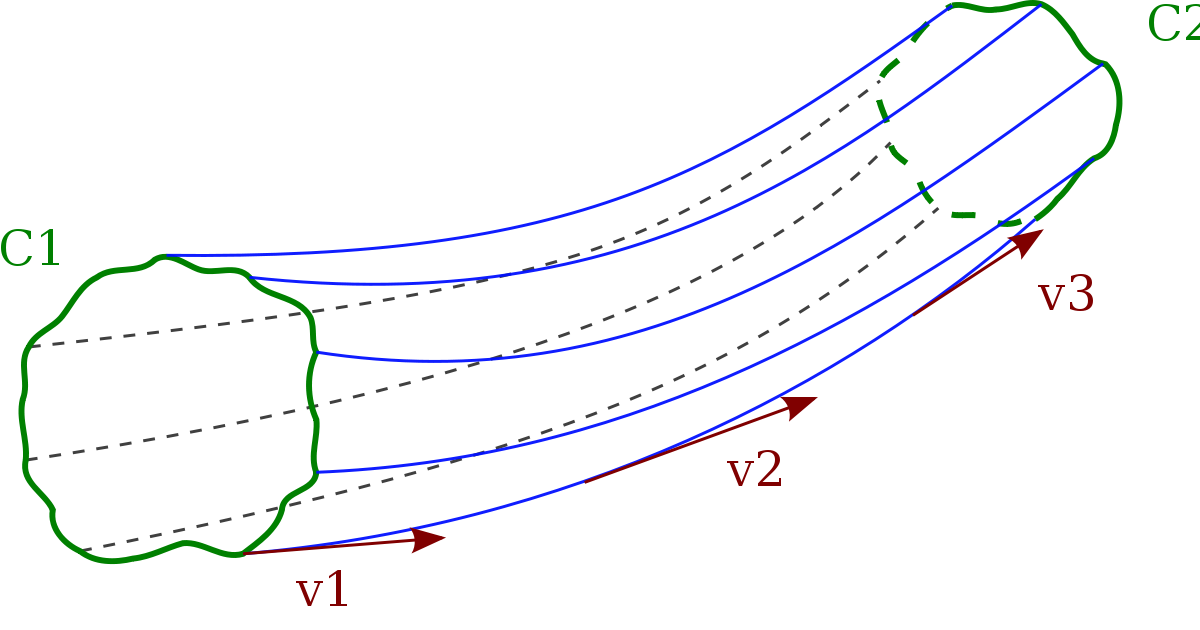
\includegraphics[width=0.6\linewidth]{images/tubo_di_flusso}
	\caption{Rappresentazione di un tubo di flusso}
	\label{fig:tubodiflusso}
\end{figure}
\FloatBarrier
La superficie laterale ha la caratteristica di avere ogni punto d$\mathbf{s}$ ortogonale al flusso $\mathbf{E}$. Osserviamo che le superfici che fanno da "tappi" del tubo di flusso (in figura C1 e C2), possono essere scelte arbitrariamente, le prendiamo in modo che i vettori $d\mathbf{s}_1$, \(d\mathbf{s}_2\) siano paralleli al vettore campo $\mathbf{E}$. Di modo che
\[\mathbf{E}\cdot d\mathbf{s}_1 = Eds_1\cos\theta= \pm |Eds_1|\]
dove il più o meno indica il fatto che a seconda del verso avremo un angolo di 0 o di 180 gradi. Ne risulta che il flusso per un tubo di flusso è
\[d\Phi = \pm |Eds_1|\pm |Eds_2| =\frac{dQ}{\varepsilon_0}\]
Consideriamo ora una superficie chiusa carica e calcoliamo il flusso di un tubo di flusso: le linee di campo partono dalla superficie divergendo verso l'esterno, scegliamo la superficie di "tappo" del tubo come appena detto. All'interno della superficie non è presente campo elettrico quindi a rigore non potremmo chiudere il tubo di flusso all'interno della superficie chiusa, possiamo però prolungare analiticamente le linee di campo all'interno e chiuderla con una superficie interna al conduttore. Sia \(S_1\) la superficie interna ed \(S_2\) quella esterna. Applichiamo ora la legge di Gauss
\[E_1ds_1+E_2ds_2 = E_2ds_2 = \frac{dQ}{\varepsilon_0}\]
\[\Rightarrow E_2 = \frac{dQ}{\varepsilon_0 ds_2}\]
Questa è l'espressione del campo elettrico passante per un tubo di flusso.\\
Si noti che \(E_2\) non è costante perché dipende dalla superficie individuata dal tubo di flusso: essendo le linee di campo divergenti dalla superficie, più ci si allontana più \(ds_2\) aumenta, facendo diminuire il campo.\\
Possiamo ora introdurre i condensatori
\begin{definizione}[Condensatore]
	Un condensatore è un componente elettrico formato da due conduttori chiamati armature, separati da un materiale isolante, ed ha la capacità di immagazzinare l'energia elettrostatica associata a un campo elettrostatico.
\end{definizione}
Applichiamo quanto ricavato ad un condensatore. Un condensatore è un apparato formato da due "armature", ovvero conduttori carichi uno positivamente ed uno negativamente, poste una di fronte all'altra. Le armature che consideriamo per ora sono poste nel vuoto. Sia A l'armatura di carica +Q e B quella di carica -Q. Vogliamo calcolare la differenza di potenziale fra le due armature, applicare la definizione di potenziale per questo calcolo è ostico perché non sappiamo come varia il campo nello spazio compreso fra le due armature. Consideriamo quindi un tubo di flusso infinitesimo che va da A a B, il campo elettrico per questo tubo è
\[E_i  = \frac{dQ_i}{\varepsilon_0 ds_i}\]
\[\Delta V_{AB} = \int_{A}^{B}\mathbf{E}d\mathbf{r} =dQ_i \int_{A}^{B}\frac{dr_i}{\varepsilon_0 ds_i}\]
In generale questo integrale è complesso da calcolare. Riordinando i termini otteniamo
\[dQ_i = \frac{\Delta V_{AB}}{\int_{A}^{B}\frac{dr_i}{\varepsilon_0 ds_i}}\]
\[Q = \sum_i\frac{\Delta V_{AB}}{\int_{A}^{B}\frac{dr_i}{\varepsilon_0 ds_i}}\]
Definiamo la \textbf{capacità di un condensatore} come
\[C\equiv \frac{1}{{ \int_{A}^{B}\frac{dr_i}{\varepsilon_0 ds_i}}}\]
osserviamo che questa quantità è una costante che dipende dalla geometria del dielettrico e dal materiale ($\varepsilon_0$ è la costante dielettrica del vuoto ma potremmo scegliere qualsiasi mezzo). L'unità di misura della capacità è il Farad (\(F\)) definito come un Coulomb su un Volt. 
\[1F \equiv \frac{1C}{1V}\]
questa capacità è enorme tanto che, in un circuito comune la capacità figura spesso il microFarad (\(\mu F\)).\\
La precedente relazione quindi si riscrive come
\[C = \frac{Q}{\Delta V}\]
Si faccia attenzione al fatto che se si diminuisce la carica nel condensatore la capacità non diminuisce perché, come detto, è una costante dipendente solo da geometria e materiale; ciò che avviene è che diminuendo la carica diminuisce anche la differenza di potenziale, mantenendo il valore di C invariato.\\
Per il calcolo della capacità in generale si seguono 3 step
\begin{enumerate}
\item Calcolare $\mathbf{E}$ tra le facce del condensatore
\item Calcolare la differenza di potenziale fra le armature \(\Delta V\)
\item Calcolare la capacità con la relazione \(C=\frac{Q}{\Delta V}\) facendo attenzione che l'espressione finale della capacità non dipenda da Q. 
\end{enumerate} 
\subsubsection*{Condensatore a facce piane parallele infinite}
Consideriamo due superfici piane parallele infinite di carica uguale ma in segno opposto. Possiamo intuitivamente ottenere dove si dispongono le linee di campo, per farlo consideriamo le linee di campo di ogni armatura singolarmente per poi unirle con il principio di sovrapposizione: la faccia di carica positiva produce un campo uscente e perpendicolare ad essa sia nel lato sinistro del condensatore, sia al centro sia nel lato destro; l'armatura carica negativamente produce linee di campo in modo analogo ma di verso opposto. Sovrapponendo le linee si ottiene che quelle nel lato sinistro e destro si eliminano (i campi generati hanno la stessa intensità essendo medesima la carica) mentre nella regione interna al condensatore le linee di campo hanno stessa direzione e verso quindi si sommano dando linee di modulo doppio.
\begin{figure}[h!]
	\centering
	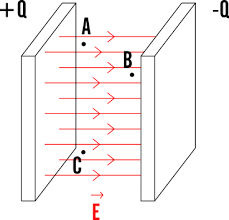
\includegraphics[width=0.4\linewidth]{images/condensatore-piano}
	\caption{Schema di un condensatore a facce piane parallele infinite, le linee di campo sono presenti solo fra le due armature e vanno dall'armatura carica positivamente a quella carica negativamente.}
	\label{fig:condensatore-piano}
\end{figure}
\FloatBarrier
Possiamo ricavare da ciò in modo formale che le cariche si dispongono sulla superficie interna (osservato precedentemente con ragionamenti non formali) applicando la legge di Gauss scegliendo un cilindro che attraversa l'armatura partendo dall'interno ed attraversando una faccia esterna: il flusso sulla superficie laterale è sicuramente nullo perché perpendicolare al campo, sulla faccia interna del cilindro è nulla perché questa è perpendicolare al campo, sulla faccia esterna è nulla perché come osservato precedentemente il campo è presente solo all'interno del condensatore (fra le due armature). 
\[\oint \mathbf{E}d\mathbf{s}= \frac{Q_{tot}}{\varepsilon_0}=0\]
Se le cariche non stanno all'interno nè sulla superficie esterna saranno allora sulla superficie interna.\\
Per ottenere la Capacità di questo condensatore seguiamo i 3 step: calcoliamo il campo elettrico fra le armature.
Per farlo calcoliamo il flusso per la faccia interna del condensatore considerando un cilindro che parte dall'interno dell'armatura e termina all'esterno attraversando la faccia interna. Osservando che l'integrale sulla superficie del cilindro è l'Area di base A e che il flusso nella faccia del cilindro interna all'armatura è nullo, si ha, eguagliando con il teorema di Gauss
\[\oint\mathbf{E}d\mathbf{s} = EA = \frac{\sigma A}{\varepsilon_0}\]
\[\Rightarrow E = \frac{\sigma}{\varepsilon_0}\]
Si noti che apparentemente questo risultato sembra contraddire quanto ottenuto in precedenza: abbiamo precedentemente dimostrato infatti ( esercizio (\ref{es:campo_piano_infinito})) che il campo generato da una superficie carica è $\frac{\sigma}{2\varepsilon_0}$. In realtà il campo calcolato è la somma del campo prodotto dalle due armature poiché inizialmente, applicando il principio di sovrapposizione al calcolo delle linee di campo, abbiamo sommato i due contributi che, essendo uguali, sono di $\frac{\sigma}{2\varepsilon_0}$ ciascuno. Si noti inoltre che sia considerati separatamente sia considerati a seguito della sovrapposizione dei campi la discontinuità è sempre $\frac{\sigma}{\varepsilon_0}$, come precedentemente dimostrato (quando si considerano insieme il campo all'interno e dietro le armature è nullo).
Una volta ottenuto il campo elettrico calcoliamo la differenza di potenziale fra le due facce 
\[\Delta V_{AB} = \int_{A}^{B}\mathbf{E}d\mathbf{r} = Ed=\frac{\sigma d}{\varepsilon_0}=\frac{Q d}{S\varepsilon_0}\]
calcoliamo infine C
\[C = \frac{Q}{\Delta V} = \frac{S\varepsilon_0}{d}\]
come previsto C non dipende da Q ma solamente dalla geometria e dal materiale.\\
Un'ultima considerazione: l'approssimazione a facce infinite è abbastanza buona ma in un condensatore finito non tiene conto che nel bordo le linee di campo non sono perpendicolari alle facce ma curvano. 
\begin{figure}[h!]
	\centering
	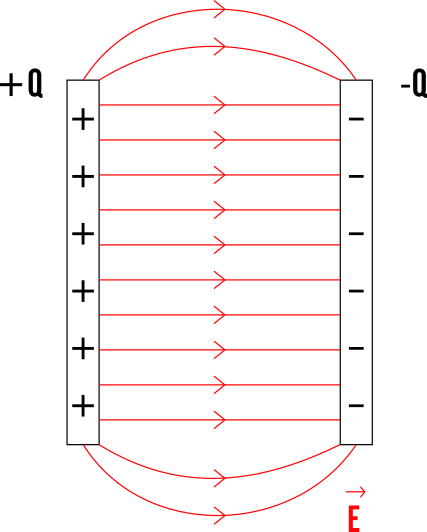
\includegraphics[width=0.4\linewidth]{images/condensatore-piano-2}
	\caption{Le linee di campo di un condensatore finito curvano in corrispondenza dei bordi}
	\label{fig:condensatore-piano-2}
\end{figure}
\FloatBarrier
\subsection*{Condensatori piani in parallelo}
\begin{definizione}[Collegamento in parallelo]
Si parla di collegamento in parallelo quando n componenti sono collegati ad una coppia di conduttori in modo che la differenza di potenziale sia la stessa per ciascun componente.
\end{definizione}
Consideriamo due condensatori collegati in parallelo come in figura
\begin{figure}[h!]
	\centering
	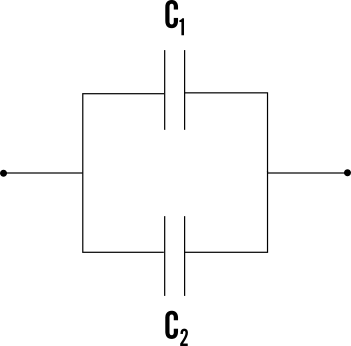
\includegraphics[width=0.4\linewidth]{images/Condensatori_parallelo}
	\caption{Schema di due condensatori collegati in parallelo}
	\label{fig:condensatoriparallelo}
\end{figure}
\FloatBarrier
dove le due facce a sinistra sono cariche positivamente rispettivamente di \(+Q_1,\ +Q_2\) e le due a destra negativamente con carica \(-Q_1,\ -Q_2\). Sia \(V_a\) il potenziale del blocco a sinistra e \(V_b\) quello a destra. Vogliamo ricavare un'espressione della capacità totale del sistema di condensatori, note le capacità \(C_1\), \(C_2\). 
\[\Delta V = V_a - V_b = \frac{Q_{tot}}{C_{tot}}\] 
\[Q_{tot}=Q_1+Q_2=C_{tot}\Delta V = (C_1+C_2)\Delta V\]
\[\Rightarrow C_{tot} = C_1 +C_2\]
Dunque la capacità risultante da un sistema di condensatori in parallelo è pari alla somma delle capacità dei singoli condensatori. In generale
\[C_{tot} = \sum_i C_i\]
Questo risultato era prevedibile in quanto in un condensatore piano la capacità dipende dalla superficie e mettere condensatori in parallelo equivale ad aumentarla. 
\subsection*{Condensatori piani in serie}
\begin{definizione}[Collegamento in serie]
	Si parla di collegamento in serie quando n componenti sono collegati in modo da essere attraversati da una corrente elettrica (che definiremo in seguito) di uguale intensità. La differenza di potenziale dei diversi componenti collegati in serie può essere diversa per ciascun componente.
\end{definizione}
Consideriamo due conduttori in serie come in figura
\begin{figure}[h!]
	\centering
	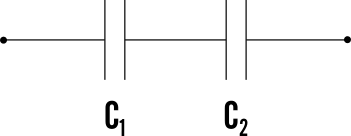
\includegraphics[width=0.6\linewidth]{images/Condensatori_serie}
	\caption{Schema di due condensatori collegati in serie}
	\label{fig:condensatoriserie}
\end{figure}
\FloatBarrier
Siano \(V_a\) \(V_e\) \(V_b\) rispettivamente i potensziali del blocco a sinistra, al centro e a destra. Notiamo subito che a differenza del caso precedente abbiamo due \(\Delta V\) diverse tra i condensatori e ci sono tre armature indipendenti. Notiamo che, non essendo collegata a nulla, l'armatura centrale E è neutra ed equipotenziale dunque sulle due facce di E ci deve essere la stessa carica, a sinistra negativa e a destra positiva. Ne segue che le cariche sono, rispettivamente, per ogni armatura, da sinistra a destra, +Q, -Q, +Q, -Q. 
\[\Delta V_{tot} = \frac{Q}{C_{tot}} = \Delta V_{ab}\]
\[\Delta V_{ab} = V_a-V_b=V_a-V_e+V_e-V_b = \frac{Q}{C_1}+\frac{Q}{C_2}\]
\[\frac{1}{C_{tot}} = \frac{1}{C_1} + \frac{1}{C_2}\]
\subsection{Condensatori dal punto di vista energetico}
Possiamo vedere un condensatore come un serbatoio di energia, vogliamo trovare un'espressione della quantità di energia immagazinata. Cominciamo chiarendo i termini del problema
\begin{definizione}[Energia]
L'energia è la capacità di un sistema o di un corpo di fare lavoro positivo
\end{definizione}
Da questa definizione risulta chiaro perché il lavoro di una forza conservativa, esprimibile come differenza di energia potenziale, è definito come \(U(A)-U(B)\) e non come \(U(B)-U(A)\) (nonostante la scelta sia arbitraria): in questo modo fare lavoro positivo vuol dire passare da uno stato iniziale ad energia maggiore U(A) per arrivare ad uno ad energia minore U(B) dove la differenza di energia è proprio il lavoro positivo fatto.\\
Osserviamo che l'energia immagazzinata in un condensatore discende dall'alta densità di carica in equilibrio nel sistema. L'energia immagazzinata deve coincidere (per la conservazione dell'energia) con il lavoro positivo fatto per portare le cariche da distanza infinita alla posizione che occupano nel condensatore. Possiamo considerare il lavoro necessario per avvicinare le cariche ad una ad una e poi generalizzare ad n cariche. Per la prima carica il lavoro è nullo, infatti possiamo scegliere il sistema di riferimento con al centro questa carica. per la seconda dobbiamo constrastare la forza di Coulomb dall'infinito fino ad \(r_{12}\), dobbiamo quindi applicare una forza $\mathbf{F}_{est} = -\mathbf{F}_{c}$.
\[L = -\int_{r_12}^{+\infty}\mathbf{F}_{c}d\mathbf{r} = -Q_2\int_{r_12}^{+\infty}\mathbf{E}d\mathbf{r} = Q_2V(r_{12}) = \frac{1}{4\pi\varepsilon_0}\frac{Q_1 Q_2}{r_{12}} = Q_1\frac{1}{4\pi\varepsilon_0}\frac{ Q_2}{r_{12}} = Q_1V(r_{21}) \]
\[\Rightarrow U_{12} = U_{21}\]
L'energia necessaria è quindi \(U_{12} = U_{21}\) 
Mettiamo ora la terza carica 
\[U_{13} = U_{31} = \frac{1}{4\pi\varepsilon_0}\frac{Q_1 Q_3}{r_{13}}\]
\[U_{23} = U_{32} = \frac{1}{4\pi\varepsilon_0}\frac{Q_2 Q_3}{r_{23}}\]
Dunque l'energia necessaria totale è 
\[U_{tot} =U_{13} + U_{23} + U_{12}  = \frac{U_{13} + U_{23} + U_{12} + U_{31} + U_{32} + U_{21}}{2}\]
Generalizzando ad n cariche
\[U_{tot} =\frac{1}{8\pi\varepsilon_0} \sum_i Q_i\sum_{j\neq i} \frac{Q_j}{r_{ij}} = \frac{1}{2}\sum_i Q_i V_i\]
dove quest'ultimo passaggio è stato possibile perché \(r_{ij} = r_{ji}\) ed esserndo il prodotto fra cariche commutativo \(Q_iQ_j = Q_jQ_i\).\\
Per passare ad una distribuzione di carica continua osserviamo
\[Q_i \to dq = \rho d\tau\]
dove $\rho$ è la densità di carica volumetrica e $\tau$ un volume infinitesimo. Ne segue
\[U_{tot} = \frac{1}{2}\int_{\tau} V\rho d\tau\]
Osserviamo ora che sull'armatura A sta una carica \(Q_a = C(V_a - V_b)\) e sull'armatura B \(Q_b = - Q_a\). L'energia totale del condensatore è
\[U_{tot} = \frac{1}{2}\sum_{i=1}^{2} Q_i V_i = \frac{1}{2} (Q_a V_a + Q_b V_b)= \frac{1}{2}C((V_a - V_b) V_a - (V_a - V_b) V_b) = \]
\[\frac{1}{2}C\Delta V^2 = \frac{1}{2}Q\Delta V = \frac{1}{2}\frac{Q^2}{C}\]
Possiamo seguire una strada concettuale diversa per ottenere il medesimo risultato: consideriamo due conduttori scarichi posti uno di fronte all'altro ed immaginiamo di spostare ad una ad una le cariche positive dell'armatura destra verso quella sinistra. La prima non necessita lavoro perché tutto è neutro ma già a partire dalla seconda esiste un campo $\mathbf{E}$ generato dalla prima carica spostata che produce una forza che si oppone al movimento da destra a sinistra della carica. Consideriamo il lavoro infinitesimo necessario per spostare di d$\mathbf{z}$ la carica dq da destra a sinistra. 
\[dL = dq\mathbf{E}d\mathbf{z} = -dqdV \]
dove il segno negativo deriva dal fatto che lo spostamento è in direzione opposta a quella del campo. Il lavoro esterno da "immettere" nel sistema è di segno opposto a quello che deve fare il sistema quindi
\[dL_{est} = -dL = dqdV\]
per ottenere il lavoro per spostare una carica dq da destra a sinistra integriamo sul percorso AB, indichiamo questo lavoro discreto con \(\Delta L\).
\[\Delta L_{est} = \int_{A}^{B} dL = \int_{A}^{B} dqdV = dq \Delta V_{ab}(q) \]
dove la differenza di potenziale dipende da q perché più cariche spostiamo da sinistra a destra più aumenta il potenziale. Per trovare il lavoro totale integriamo per tutte le cariche
\[L_{est} = \int_0^Q  \Delta V_{ab}(q) dq= \int_0^Q \frac{qdq}{4\pi\varepsilon_0 d} = \frac{q^2}{8\pi\varepsilon_0 d} = \frac{1}{2}Q\Delta V = \frac{1}{2} C \Delta V^2\]
Ma l'energia immagazzinata dove risiede? Abbiamo appena visto che spostando le cariche aumenta la differenza di potenziale e quindi il campo elettrico, l'energia è immagazzinata nel campo elettrico: in generale dove c'è campo elettrico c'è energia.\\
Possiamo sostituire all'ultima espressione ottenuta due espressioni viste in precedenza per la capacità di un condensatore piano e per la differenza di potenziale di questo 
\[U_{tot} = [\frac{1}{2}\varepsilon_0 E^2](Sd) \]
\[u_e \equiv \frac{1}{2}\varepsilon_0 E^2\]
quest'ultima è detta "densità di energia", in questo caso è stata ricavata per un condensatore piano a facce parallele ma vedremo in seguito che questo è un caso particolare di un teorema molto più generale, il teorema di Poynting, e che questo è sempre il valore della densità di energia (locale) del campo elettrico.
\section{Dipoli elettrici}
\begin{definizione}[Dipolo elettrico]
	Un dipolo elettrico, in elettrostatica, è un sistema composto da due cariche elettriche uguali e di segno opposto e separate da una distanza costante nel tempo.
\end{definizione}
\begin{figure}[h!]
	\centering
	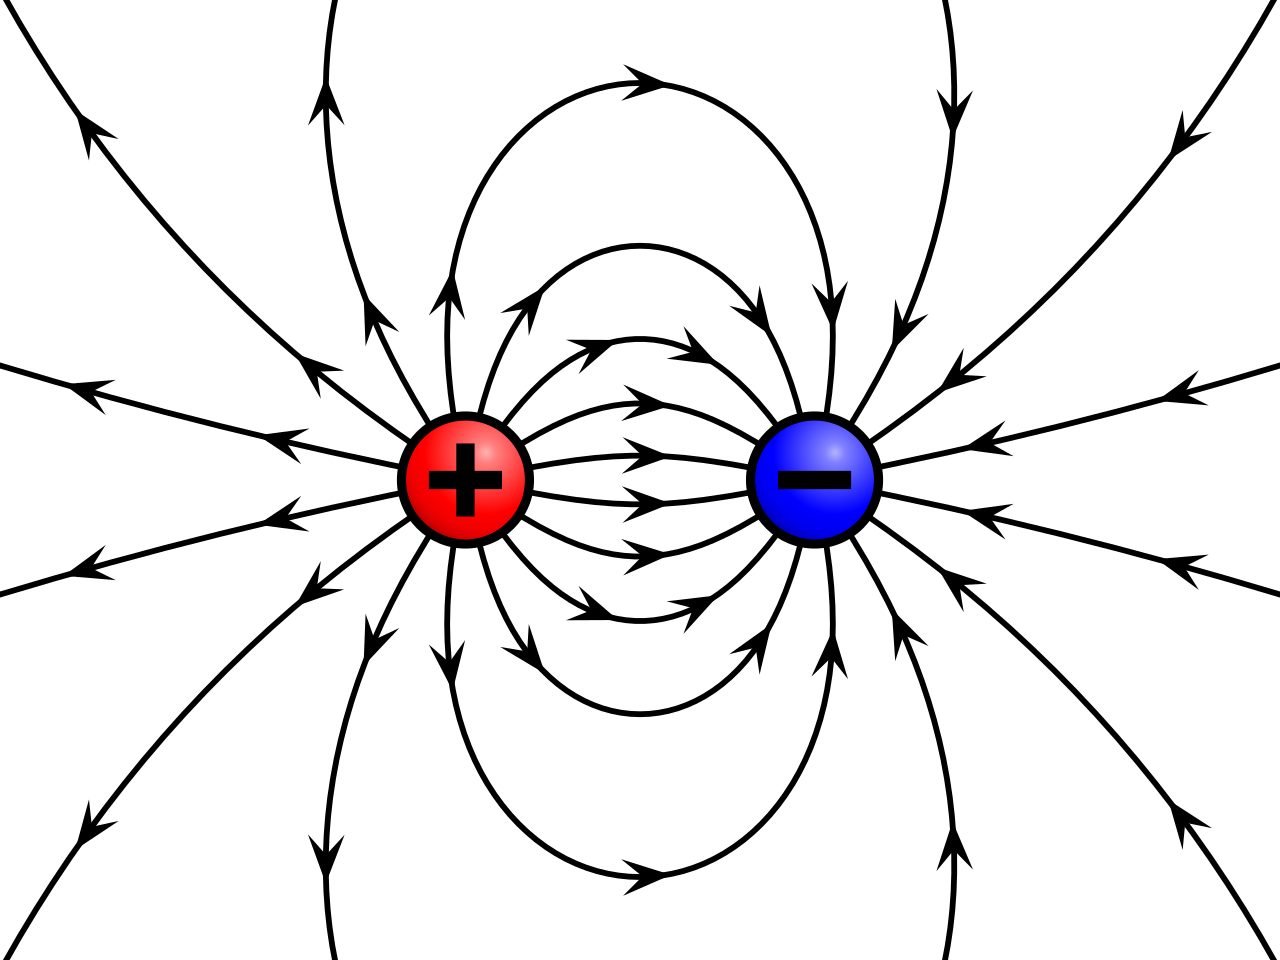
\includegraphics[width=0.4\linewidth]{images/dipolo_elettrico}
	\caption{Schema delle linee di campo di un dipolo elettrico.}
	\label{fig:dipoloelettrico}
\end{figure}
\FloatBarrier
Usando solamente il principio di sovrapposizione possiamo ottenere il campo generato da un dipolo elettrico su un punto posto sullo stesso asse del dipolo.
\begin{esercizio}[Campo elettrostatico generato da due cariche puntiformi]
	Si considerino due cariche poste per semplicità entrambe sull'asse z e a distanza uguale dall'origine (una dal lato positivo ed una dal lato negativo) e di distanza d fra di esse, vogliamo ottenere un'espressione del campo elettrico che genera in un punto P che giace sull'asse y a distanza r dall'asse z. Si noti che questo è un caso particolare (date le simmetrie geometriche con cui abbiamo costruito il sistema) in cui è presente solo una componente parallela al dipolo. Consideriamo inizialmente due cariche di segno opposto (quella positiva sopra e quella negativa sotto), si traccino i vettori \(\mathbf{r}_+ \ \mathbf{r}_- \) congiungenti le cariche al punto P, dato il segno negativo della carica in basso, il vettore campo avrà verso entrante (verso la carica) mentre il campo generato dalla carica in alto è uscente dalla carica e quindi diretto verso il punto P. Sommando i vettori di campo otteniamo che il campo risultante ha direzione parallela all'asse z e verso negativo (-$\hat{\mathbf{k}}$). Chiamiamo y il modulo della proiezione sull'asse z del vettore $\mathbf{r}_+$.
	\[\hat{\mathbf{r}}_+ =\frac{ 0\hat{\mathbf{i}}+y \hat{\mathbf{j}}-\frac{d}{2}\hat{\mathbf{k}}}{r}\]
	\[\hat{\mathbf{r}}_- = \frac{0\hat{\mathbf{i}}+y \hat{\mathbf{j}}+\frac{d}{2}\hat{\mathbf{k}}}{r}\]
	\[\mathbf{E}_{//} = \mathbf{E}_{+} + \mathbf{E}_{-} = \frac{1}{4\pi\varepsilon_0}\frac{q}{r^2}\left(\hat{\mathbf{r}}_+-\hat{\mathbf{r}}_-\right)=\]
	\[\frac{1}{4\pi\varepsilon_0}\frac{q}{r^3}\left[(y\hat{\mathbf{j}}-\frac{d}{2}\hat{\mathbf{k}})-(y\hat{\mathbf{j}}+\frac{d}{2}\hat{\mathbf{k}})\right]= -\frac{1}{4\pi\varepsilon_0}\frac{q d}{r^3}\hat{\mathbf{k}}\]
	Possiamo definire una nuova grandezza legata ad una coppia di cariche opposte: il \textbf{momento di dipolo} ed esprimere il campo in funzione di esso.
	\[\mathbf{p} \equiv qd\mathbf{k}\]
	\[\mathbf{E}_{//} = \frac{1}{4\pi\varepsilon_0}\frac{\mathbf{p}}{r^3}\]
	Se invece le cariche fossero state dello stesso segno avremmo ottenuto con ragionamenti analoghi ma cambiando il segno del vettore
	\[\mathbf{E}_{\perp} = \frac{1}{4\pi\varepsilon_0}\frac{q2y}{r^3}\hat{\mathbf{j}}\]
\end{esercizio}
Finora abbiamo ottenuto solamente la componente del campo parallela al dipolo. Sfruttando il potenziale elettrostatico possiamo ottenere un'espressione più generale
\begin{esercizio}[Espressione generale del campo generato da un dipolo elettrico]
	Consideriamo un dipolo elettrico come in figura dove chiamiamo a la distanza fra le due cariche, effettuiamo l'approssimazione \(r>>a\). Sia P il punto a cui puntano i vettori \(\mathbf{r_1}, \mathbf{r_2}, \mathbf{r}\). 
	\begin{figure}[h!]
		\centering
		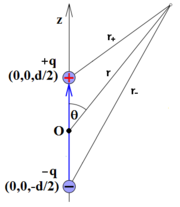
\includegraphics[width=0.4\linewidth]{images/dipolo}
		\caption{Schema di un dipolo elettrico}
		\label{fig:dipolo}
	\end{figure}
	\FloatBarrier
	Il potenziale sul punto P generato dalle due cariche è
	\[V(P) = \frac{q}{4\pi\varepsilon_0}\left(\frac{1}{r_1}-\frac{1}{r_2}\right) =  \frac{q}{4\pi\varepsilon_0}\frac{r_2-r_1}{r_1r_2}\]
	Osserviamo che per l'approssimazione fatta possiamo scrivere
	\[\Delta r = r_2-r_1 \simeq a\cos\theta\]
	\[r_1r_2 \simeq r^2\]
	\[\Rightarrow V(P) = \frac{q a \cos\theta}{4\pi\varepsilon_0 r^2}\]
	Ricordiamo che per definizione il momento di dipolo elettrico è
	\[\mathbf{p} = q\mathbf{a} = p\hat{\mathbf{k}}\]
	\[\Rightarrow V(P) = \frac{p \cos\theta}{4\pi\varepsilon_0 r^2} = \frac{\mathbf{p}\mathbf{r}}{4\pi\varepsilon_0 r^3} = \frac{pz}{4\pi\varepsilon_0 (x^2+y^2+z^2)^{\frac{3}{2}}}\]
	Calcoliamo ora le componenti parallela e perpendicolare del campo elettrico generato dal dipolo
	\[\mathbf{E}_{//} = \mathbf{E}_z = -\frac{\partial V}{\partial z} \hat{\mathbf{k}} = \frac{p(3\cos^2\theta-1)}{4\pi\varepsilon_0 r^3}\]
	dove nello svolgere i passaggi è stata usata \(z = r\cos\theta\). Analogamente possiamo calcolare il campo sull'asse x e sull'asse y
	\[E_x = -\frac{\partial V}{\partial x} \hat{\mathbf{i}}=\frac{p(3zx)}{4\pi\varepsilon_0 r^5}\]
	\[E_y = -\frac{\partial V}{\partial y} \hat{\mathbf{j}}=\frac{p(3zy)}{4\pi\varepsilon_0 r^5}\]
	\[E_{\perp} = \sqrt{E_x^2+E_y^2} = \frac{p}{4\pi\varepsilon_0r^3}3\cos\theta\sin\theta\]
	dove nei passaggi è stato usato \(r_{\perp} = \sqrt{x^2+y^2} = r\sin\theta\)
	Ne segue che se \(\theta = 0^\circ \)
	\[E_{\perp} = 0\]
	\[E_{//} = \frac{p}{2\pi\varepsilon_0r^3}\]
	mentre se \(\theta = 90^\circ\)
	\[E_{\perp} = 0^\circ\]
	\[E_{//} = -\frac{p}{4\pi\varepsilon_0r^3}\]
\end{esercizio}
Che è lo stesso risultato ottenuto nell'esercizio precedente.\\
Talvolta può risultare utile studiare un dipolo in coordinate polari quindi rispetto al raggio $\rho$ e gli angoli $\theta$ e $\gamma$. in questo caso il campo elettrico si esprime come 
\[E_\rho = -\frac{\partial V}{\partial \rho}\]
\[E_\gamma = -\frac{1}{r\sin\theta}\frac{\partial V}{\partial \gamma}\]
\[E_\theta = -\frac{1}{r}\frac{\partial V}{\partial \theta}\]
\subsection{Dipolo in un campo elettrico}
Consideriamo ora un dipolo formato da due cariche puntiformi immerso in campo elettrostatico $\mathbf{E}$
\begin{figure}[h!]
	\centering
	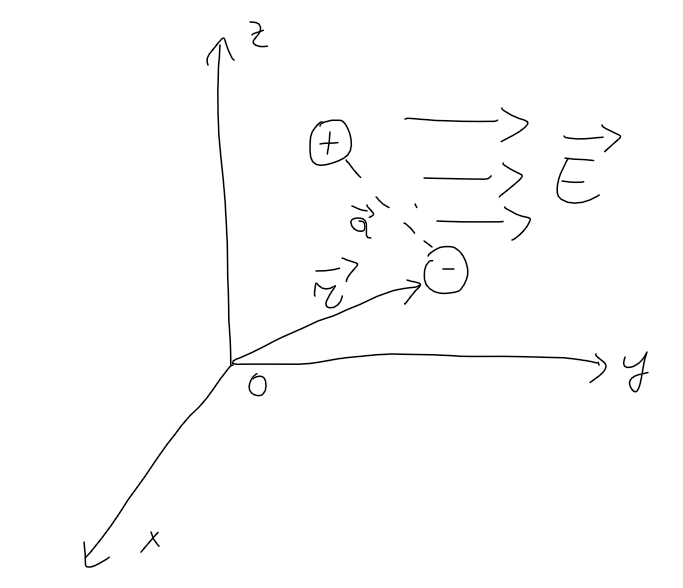
\includegraphics[width=0.5\linewidth]{images/dipolo_campo_elettrico}
	\caption{Grafico del dipolo immerso in un campo elettrico}
	\label{fig:dipolocampoelettrico}
\end{figure}
\FloatBarrier
calcoliamo l'energia potenziale del dipolo calcolando il lavoro necessario ad avvicinare le due cariche partendo dall'infinito (entrambe sotto l'effetto del campo $\mathbf{E}$)
\[L = \int_{\infty}^{\mathbf{r}+\mathbf{a}} qE(r) dr -\int_{\infty}^{\mathbf{r}} qE(r) dr =\int_{\mathbf{r}}^{\mathbf{r}+\mathbf{a}} qE(r) dr= U(\mathbf{r}+\mathbf{a})-U(\mathbf{r}) = qV(\mathbf{r}+\mathbf{a})-qV(\mathbf{r})\]
Considerato che $||\mathbf{a}||<<||\mathbf{r}||$, possiamo interpretare le componenti \((a_x, a_y, a_z)\) come tendenti a zero quindi \((a_x, a_y, a_z)\simeq (\partial x, \partial y, \partial z)\)
\[U = q[V(x+a_x, y+a_y, z+a_z)-V(x, y, z)] = qdV = q\left[\frac{\partial V}{\partial x} a_x + \frac{\partial V}{\partial y}a_y + \frac{\partial V}{\partial z}a_z\right] =\]
\[ q(-\mathbf{E}\mathbf{a}) = -\mathbf{p}\mathbf{E}\]
Da cui segue, ricordando che \(\mathbf{F} = \mathbf{\nabla} U\)
\[\mathbf{F} = \mathbf{p}\mathbf{\nabla}\mathbf{E}\]
Notiamo che abbiamo una condizione di equilibrio stabile quando questa funzione presenta un minimo, ovvero per \(\theta= 0^\circ,\ 180^\circ\). inoltre notiamo che, avendo considerato $\mathbf{a}$ infinitesimo, possiamo considerare in campo elettrico uguale nelle due cariche quindi la forza totale su un generico punto risulta 
\[\mathbf{F}_{tot} =\mathbf{F}_++\mathbf{F}_- = q\mathbf{E}-q\mathbf{E} = 0\]
Il momento delle forze totale invece è
\[\mathbf{M}_{tot} = \mathbf{r}_+\wedge\mathbf{F}_+ + \mathbf{r}_-\wedge\mathbf{F}_- = \mathbf{r}_+\wedge q\mathbf{E}_+ + \mathbf{r}_\wedge q\mathbf{E}_ = (\mathbf{r}_+ - \mathbf{r}_-)\wedge q \mathbf{E} = (\mathbf{a}q)\wedge\mathbf{E} = \mathbf{p}\wedge\mathbf{E}\]
Notiamo che essendo il momento \(pE\sin\theta\), si ha che esso è nullo per \(\theta= 0^\circ,\ 180^\circ\), gli unici angoli in cui il sistema è stabile. 
\subsection{Sistema di cariche come dipolo}
Consideriamo ora un sistema di cariche discrete (il caso uniforme è analogo ma con gli integrali al posto delle sommatorie). Per il principio di sovrapposizione possiamo esprimere il potenziale totale sul punto P come somma dei potenziali generati dalle i cariche \(q_i\).
\begin{figure}[h!]
	\centering
	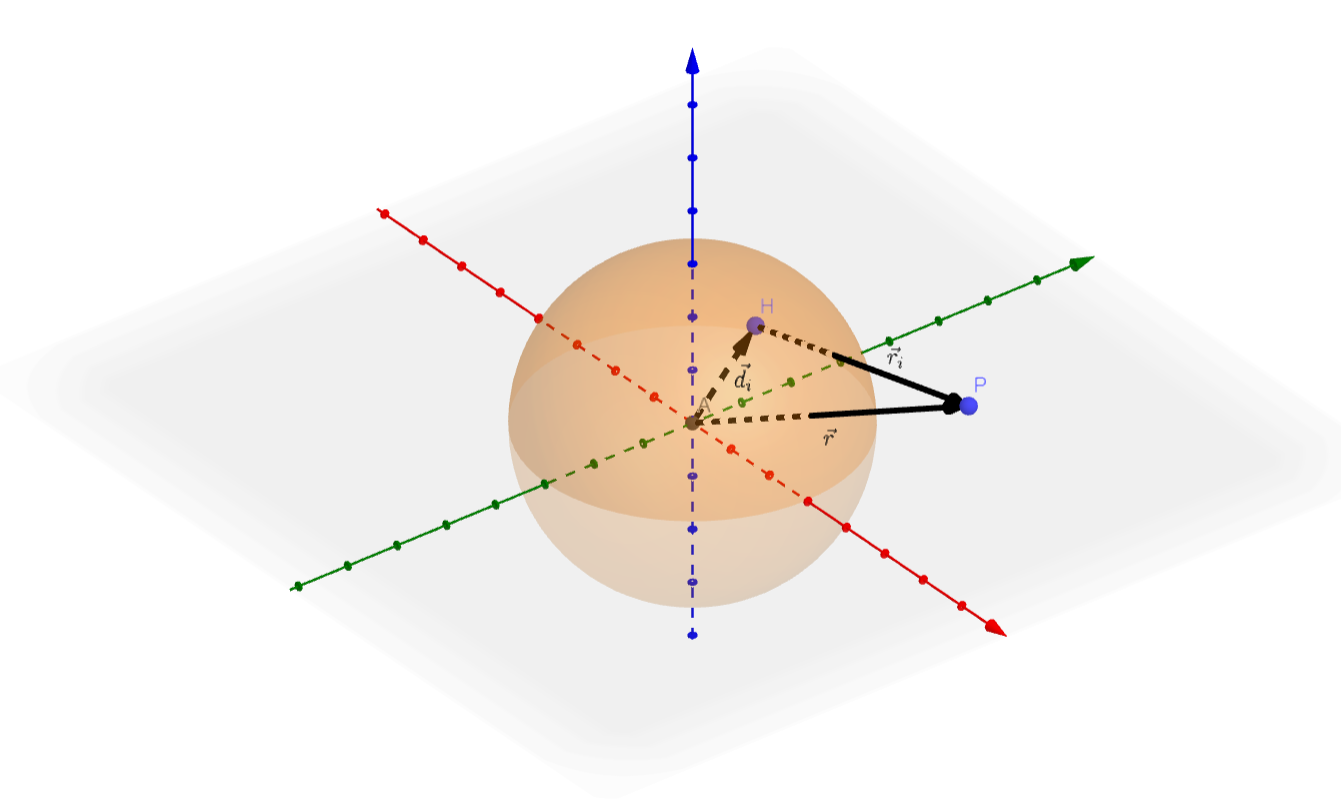
\includegraphics[width=0.5\linewidth]{images/sistema_dipolo}
	\caption{Schema del sistema di cariche}
	\label{fig:sistemadipolo}
\end{figure}
\FloatBarrier
\[V(P) = \frac{1}{4\pi\varepsilon_0}\sum_i \frac{q_i}{r_i}\]
Ipotizziamo che la dimensione d del sistema sia molto più piccola della distanza dal punto P \(d<<r\), ne seguirà che anche \(d_i<<r_i\). Possiamo dunque scrivere le seguenti relazioni
 \[\mathbf{r}_i = \mathbf{r} - \mathbf{d}_i\]
 \[r_i \simeq r-d_i\cos\theta_i\]
 \[r-r_i = d_i\cos_i = \mathbf{d}\cdot\hat{\mathbf{r}}\]
 \[\frac{1}{r_i} = \frac{1}{(r-\mathbf{d}_i\cdot\hat{\mathbf{r}})}\frac{r+\mathbf{d}_i\cdot\hat{\mathbf{r}}}{r+\mathbf{d}_i\cdot\hat{\mathbf{r}}} = \frac{r+\mathbf{d}_i\cdot\mathbf{r}}{r^2-(\mathbf{d}\hat{\mathbf{r}})^2} \simeq \frac{r+\mathbf{d}_i\cdot\mathbf{r}}{r^2}\]
 \[\Rightarrow V(P) =\frac{1}{4\pi\varepsilon_0}\sum_i \frac{q_i}{r^2}(r+\mathbf{d}_i\cdot\hat{\mathbf{r}}) = \frac{1}{4\pi\varepsilon_0}\frac{Q}{r}+\frac{1}{4\pi\varepsilon_0}\frac{(\sum_i(q_i\mathbf{d}_i))\hat{\mathbf{r}}}{r^2}\]
 Possiamo generalizzare la definizione di momento di dipolo ad un sistema discreto 
 \[\mathbf{p} = \sum_i q_i\mathbf{d}_i\]
 \[V(P) = \frac{1}{4\pi\varepsilon_0}\frac{Q}{r}+\frac{1}{4\pi\varepsilon_0}\frac{\mathbf{p}\hat{\mathbf{r}}}{r^2}\]
 Le due componenti del potenziali sono rispettivamente dette di monopolo \(V_0\) e di dipolo \(V_{dip}\), la prima equivale al potenziale che il sistema genererebbe se tutta la carica fosse concentrata in un punto mentre il secondo tiene conto della distribuzione di carica del sistema. Ne segue che anche se al carica totale Q fosse nulla, un sistema può comunque generare potenziale se le sue cariche sono disposte in certo modo. Possiamo dimostrare che il secondo membro è trascurabile rispetto al primo infatti
 \[\frac{V_{dip}}{V_0} = \frac{|\mathbf{p}\cdot \hat{\mathbf{r}}|}{rQ}\leq\frac{|\mathbf{p}|}{rQ} = \frac{|\sum_i q_i d_i|}{rQ}\leq \frac{|(\sum_i q_i)d|}{rQ} = \frac{d}{r}<<1\]
 In generale se cambio l'origine del sistema cambiano i \(q_i\) e i \(d_i\) quindi \(\mathbf{p}\neq\mathbf{p}'\). Tuttavia se \(\sum_i q_i = Q_{tot} = 0\) allora $\mathbf{p}$ diventa indipendente da come scegliamo il sistema di riferimento. 
\begin{figure}[h!]
	\centering
	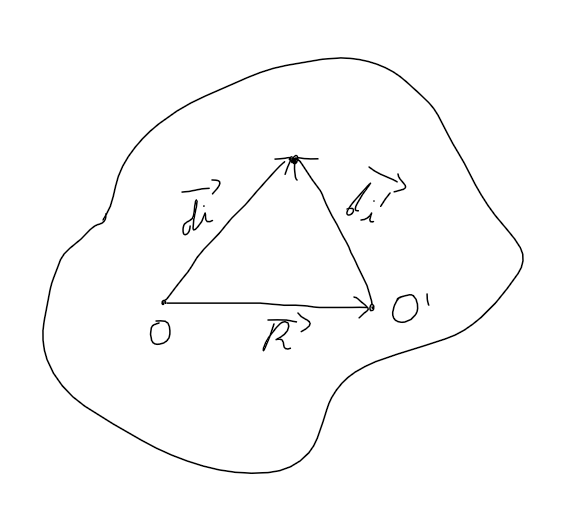
\includegraphics[width=0.5\linewidth]{images/dipolo_SR}
	\caption{Schema di uno stesso punto espresso rispetto a due diversi sistemi di riferimento i cui centri sono a distanza \(\mathbf{R}\).}
	\label{fig:dipolosr}
\end{figure}
\FloatBarrier
\[\mathbf{d}_i = \mathbf{R}+\mathbf{d}'_i\]
\[\mathbf{p} = \sum_iq_id_i = \sum_iq_i\mathbf{R}+\sum_iq_i\mathbf{d}'_i=QR+\mathbf{p}'\]
Se \(Q = 0\) si ha \(\mathbf{p} = \mathbf{p}'\). L'analogia con la statica è in questo caso evidente.\\
Ci chiediamo ora quando, se \(Q_{tot} = 0\), $\mathbf{p} = 0$. Possiamo riscrivere $\mathbf{p}$ e definire il "centro di carica" per le cariche positive e negative 
\[\mathbf{p} = \sum_iq_id_i = \sum_i|q_i^+|\mathbf{d_i}-\sum_i|q_i^-|\mathbf{d_i}\]
\[\mathbf{d}_+ = \frac{\sum_i|q_i^+|\mathbf{d_i}}{\sum_i|q_i^+|} = \frac{\sum_i|q_i^+|\mathbf{d_i}}{|Q^+|}\]
\[\mathbf{d}_- = \frac{\sum_i|q_i^-|\mathbf{d_i}}{\sum_i|q_i^-|} = \frac{\sum_i|q_i^-|\mathbf{d_i}}{|Q^-|}\]
\[\mathbf{p} = Q^+\mathbf{d}^+-|Q^-|\mathbf{d}^-\]
Se il corpo è neutro abbiamo \(|Q^+|=|Q^-|=Q\) quindi \(\mathbf{p} = Q(\mathbf{d}^+-\mathbf{d}^-)\). Ne segue che $\mathbf{p}$ è nullo se i due centri di carica coincidono. Notiamo che un qualsiasi corpo con una generica distribuzione di carica può essere visto come un dipolo elettrico. Ad esempio, nell'atomo di idrogeno si ha un nucleo positivo che ha centro di carica nel suo centro attorniato da una nuvola elettronica sferica \(1s^1\) con centro nel centro dell'atomo, i due centri di carica coincidono e l'atomo d'idrogeno presenta momento di dipolo nullo. L'acqua invece, avendo la tipica forma a V, ha centri di carica positiva e negativa diversi da cui discende la forte polarità della molecola d'acqua. Inoltre, anche se un atomo 
\begin{figure}[h!]
	\centering
	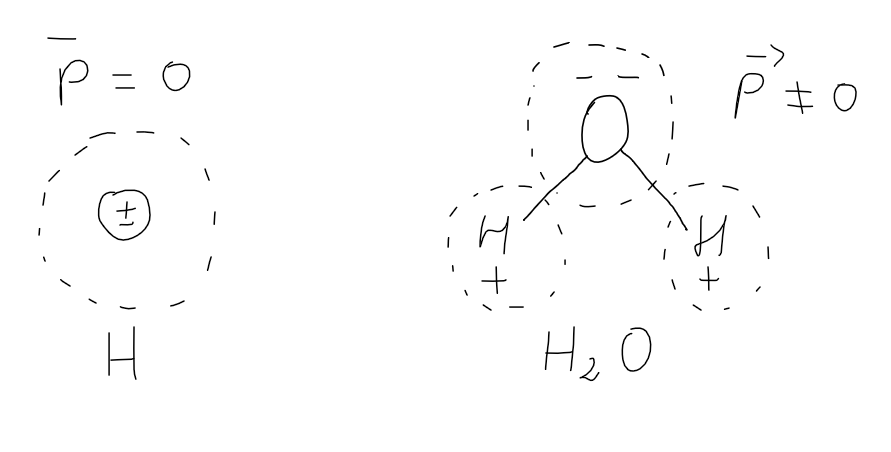
\includegraphics[width=0.5\linewidth]{images/dipolo_H_H2O}
	\caption{L'idrogeno non presenta momento di dipolo mentre l'acqua si.}
	\label{fig:dipolohh2o}
\end{figure}
\FloatBarrier
\section{Dielettrici}
Come già accennato, un dielettrico è un materiale schematizzabile come un reticolo cristallino in cui tutti gli elettroni sono legati. Ha proprietà isolanti ed è contrapposto ai materiali conduttori.\\
Un dielettrico, nonostante abbia gli elettroni "fissi" può polarizzarsi se esposto ad un campo elettromagnetico.
\begin{figure}[h!]
	\centering
	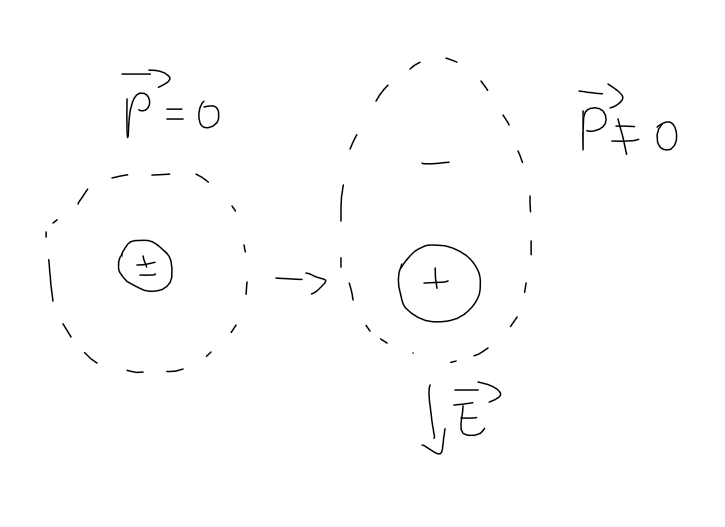
\includegraphics[width=0.6\linewidth]{images/dielettrico_idrogeno}
	\caption{Un dielettrico sottoposto ad un campo elettrico si polarizza.}
	\label{fig:dielettricoidrogeno}
\end{figure}
\FloatBarrier
\begin{definizione}[Dielettrico]
	Qualsiasi sostanza non conduttrice che, immersa in un campo elettrico esterno, dà luogo a fenomeni di polarizzazione più o meno intensi, che producono una variazione del campo elettrico totale.
\end{definizione}
Consideriamo un condensatore a facce piane parallele, se fra le armature vi è il vuoto abbiamo le seguenti informazioni:
\[C_0 = \frac{\varepsilon_0S}{d}\]
\[|\mathbf{E}_0| = \frac{\sigma}{\varepsilon_0} = \frac{Q}{\varepsilon_0 S}\]
\[\Delta V_0 = \int_{0}^{d}\mathbf{E}d\mathbf{r} = Ed = \frac{Q}{C_0}\]
Se però fra le armature poniamo una lastra metallica (conduttrice) di spessore D, otteniamo
\[\Delta V = \int_{0}^{d}\mathbf{E}d\mathbf{r} = \int_{0}^{d'}\mathbf{E}d\mathbf{r} + \int_{d'+D}^{d}\mathbf{E}d\mathbf{r} = Ed' + E(d-(d'+D)) = E(d-D) < \Delta V_0 \]
La differenza di potenziale diminuisce di ED e questa quantità è indipendente dalla posizione della lastra rispetto le due armature (se sia più vicina ad una o all'altra).\\
Se poniamo una lastra di dielettrico invece la differenza di potenziale riduce ma in quantità minore. Se aumentiamo lo spessore D la differenza di potenziale diminuisce fino ad un minimo (quando il dielettrico occupa tutto lo spazio fra le armature quindi \(D = d\)) $\Delta V_k$. Si nota sperimentalmente che 
\[\Delta V_k = \frac{\Delta V_0}{k}\]
dove k è una costante adimensionale che dipende dal materiale detta "costante dielettrica relativa" (contrassegneremo con una k al pedice le grandezze caratteristiche di sistemi in cui è presente un dielettrico di costante dielettrica relativa k). Possiamo ricalcolare tutte le quantità prima elencate
\[C_k = \frac{Q}{\Delta V_k} = \frac{Qk}{\Delta V_0} = kC_0 = \frac{(k\varepsilon_0)S}{d} = \frac{\varepsilon S}{d}\]
dove $\varepsilon = k\varepsilon_0$ è la costante dielettrica del materiale. 
\[\Delta V_k = \frac{\Delta V_0}{k} = \frac{1}{k}\int_{0}^{d}\mathbf{E}d\mathbf{r} = \int_{0}^{d}\mathbf{E}_kd\mathbf{r} = E_kd = \frac{E}{k}d \]
\[\Rightarrow E_k = \frac{E}{k}= \frac{\sigma}{\varepsilon_0 k} = \frac{\sigma_k}{\varepsilon_0}\]
\[\Rightarrow \sigma_k = \frac{\sigma}{k}\]
dove $\sigma_k$ è la densità di carica sulla superficie del condensatore.\\
La densità di carica sulla superficie del condensatore è più bassa di quella che ci sarebbe se il dielettrico non ci fosse; ipotizziamo (lo dimostreremo) che questa diminuzione di carica è dovuta al fatto che sulla superficie del dielettrico è presente una densità di carica di segno opposto \(\sigma_p\). Sappiamo che anche nel caso del dielettrico come in quello del conduttore le cariche stanno in superficie perché, se applichiamo la legge di Gauss considerando un cilindro che parte dall'armatura superiore e finisce all'interno del dielettrico, indipendentemente dall'altezza dal cilindro, troviamo lo stesso valore di carica totale al suo interno.
\[\oint_\Sigma \mathbf{E}d\mathbf{s} = \frac{Q_{tot}}{\varepsilon_0} = E_k A \]
la carica totale è indipendente dall'altezza del cilindro scelto quindi la carica non può stare all'interno del cilindro.\\
Riprendendo la precedente espressione, possiamo scrivere
 \[\frac{Q_{tot}}{\varepsilon_0} = E_k A = \frac{\sigma A - \sigma_p A}{\varepsilon_0}\]
dove abbiamo sottratto alla $\sigma$ che ci sarebbe in un conduttore alla $\sigma_p$, si noti che siamo sicuri della presenza di una $\sigma_p$ di segno opposto a quella dell'armatura  sappiamo che \(\sigma_k<\sigma\) e quindi possiamo scrivere \(\sigma_k = \sigma -\sigma_p\). Possiamo quindi svolgere le seguenti considerazioni
\[E_k = \frac{\sigma }{\varepsilon_0 k} = \frac{\sigma}{\varepsilon_0}\left[\frac{1}{k}-1+1\right] = \frac{\sigma}{\varepsilon_0}\left[1-\frac{k-1}{k}\right] = \frac{\sigma}{\varepsilon_0}-\frac{\sigma_p}{\varepsilon_0}\]
\[\Rightarrow \sigma_k = \frac{k-1}{k}\sigma\]
Notiamo che più k è grande più grande è la carica di polarizzazione.\\
Fin ora abbiamo solamente tratto deduzioni matematiche senza chiederci il motivo fisico per cui otteniamo questi risultati. Ciò che avviene è analogo a quanto visto per l'atomo di idrogeno in un campo elettrico: le nuvole elettroniche degli atomi nel dielettrico si spostano creando una polarizzazione. 
\[\mathbf{\delta} = \mathbf{d}_+ -\mathbf{d}_- \neq 0\]
\[\mathbf{p} = q\mathbf{\delta}\neq 0\]
dove questo momento di dipolo è quello generato da un singolo atomo. La polarizzazione avviene in tutti gli atomi del dielettrico ma negli strati interni la asimmetria di carica di uno strato è compensata da quello superiore ed inferiore; la polarizzazione crea dunque una densità di carica solo in superficie dove non è presente uno strato superiore o inferiore. Abbiamo così spiegato il perché della presenza di \(\sigma_p\) da cui scaturiscono le relazioni matematiche appena dedotte. Definiamo il \textbf{vettore di polarizzazione} come
\[\mathbf{P} = n\mathbf{p} = nq\mathbf{\delta} = \frac{\Delta N}{\Delta \tau} q \mathbf{\delta} \]  
dove n è la densità volumetrica di atomi e q è la carica di un'atomo (considerato come un dipolo) data da \(q = ze\) dove z è il numero atomico. Notiamo inoltre che più aumenta il campo elettrico più aumenta $\mathbf{\delta}$ e quindi anche il vettore di polarizzazione.\\
Si nota sperimentalmente (ma si dedurrà a breve) che la maggior parte dei dielettrici rispettano la seguente relazione
\begin{align}\label{eq:polarizzazione_lineare}
	\mathbf{P} = \varepsilon_0(k-1)\mathbf{E} = \varepsilon_0 \chi \mathbf{E}
\end{align}
dove $\chi$ è detta \textbf{suscettibilità elettrica}. I dielettrici che rispettano questa condizione sono detti lineari perché p dipende linearmente da E, limiteremo la nostra trattazione a questo tipo di materiali. Di solito P è uniforme all'interno del dielettrico ma esistono casi in cui cambia, di conseguenza anche k cambia all'interno del materiale. Inoltre nella maggior parte dei casi \(\mathbf{P} // \mathbf{E}\) (per come abbiamo scritto l'ultima equazione sembra l'unica opzione possibile) tuttavia può accadere che k non sia uno scalare am un tensore 3x3, in questo caso la direzione di $\mathbf{P}$ può non essere la stessa di $\mathbf{E}$. Quando ciò avviene il materiale è detto anisotropo (ad esempio i cristalli birifrangenti). Fin ora abbiamo quindi studiato solamente dielettrici lineari isotropi.
\begin{definizione}[Velocità isotropa]
	L'isotropia è la proprietà dell'indipendenza dalla direzione, da parte di una grandezza definita nello spazio. Il suo contrario è l'anisotropia.
\end{definizione}
\subsection{Interpretazione microscopica della polarizzazione di un dielettrico}
Abbiamo visto che quando avviene la polarizzazione si ridistribuiscono le cariche e si genera una densità di carica sulla superficie \(\sigma_p\), abbiamo giustificato matematicamente il fatto che questa si generi proprio in superficie con la legge di Gauss e ne abbiamo reso conto anche fisicamente mediante un'interpretazione microscopica della polarizzazione.\\
A causa di questa ridistribuzione di carica si crea un campo elettrico indotto di entità molto minore rispetto a quello che viene a crearsi in un conduttore (dove la polarizzazione è totale, cioè si ferma solo quando il campo elettrico esterno è totalmente schermato); la schermatura del campo esterno è quindi molto minore rispetto ad un conduttore e la differenza di potenziale fra le armature del condensatore si riduce in quantità minore. Continuerà dunque ad esistere un campo elettrico all'interno del dielettrico $\mathbf{E}$ (a differenza del caso del conduttore)
\[\mathbf{E} = \mathbf{E}_0+\mathbf{E}_p<\mathbf{E}_0\]
dove $\mathbf{E}_0$ è il campo esterno che già era presente e $\mathbf{E}_p$ è il campo di polarizzazione (che si oppone a quello preesistente).\\
Basandoci su questa interpretazione microscopica ci chiediamo quanto valga $\sigma_p$. Conoscendo la densità volumetrica di atomi nel dielettrico (n), la moltiplichiamo alla carica di un singolo atomo (ottenendo la densità di carica del dielettrico), che poi moltiplichiamo per uno spessore infinitesimo (\(\delta\)) corrispondente alla distanza fra i centri di carica positiva e negativa del singolo atomo, ottenendo così la densità superficiale.
\[\sigma_p = n q \delta\]
Ricordando che \(\mathbf{P} = nq\mathbf{\delta}\), abbiamo che $\sigma_p = |\mathbf{P}|$. Se però il campo non è perpendicolare alla superficie del dielettrico ma vi entra con un angolo di incidenza $\theta$, allora la distanza fra i centri di carica negativo e positivo sarà di modulo $\delta$ ma orientata obliquamente, parallela al campo elettrico. Ne segue che la densità di carica decresce secondo il coseno dell'angolo di incidenza, possiamo quindi scrivere una forma più generale della densità superficiale di polarizzazione
\[\sigma_p = np\delta \cos\theta= |\mathbf{P}|\cos\theta = \mathbf{P}\hat{n}\]
Solitamente la densità di carica dovuta alla polarizzazione sta sulla superficie per i motivi precedentemente spiegati, tuttavia fin ora abbiamo implicitamente presunto che il dielettrico sia omogeneo, cioè, intuitivamente, che non presenti irregolarità al suo interno.
In generale, a livello locale, visto che può capitare che se il materiale non è "regolare", non tutte le cariche generate dalla polarizzazione di uno strato interno siano annullate da quelli adiacenti; si possono quindi avere cariche anche all'interno del dielettrico (vi sarà quindi una densità di carica volumetrica dovuta alla polarizzazione \(\rho_p\)).\\
Vediamo una trattazione matematica di questo fenomeno. Consideriamo una superficie $\Sigma$ all'interno del dielettrico, se non c'è campo esterno non c'è polarizzazione quindi abbiamo abbiamo
\[E = V(\Sigma) Q = 0\]
\[Q_p = \int_{V(\Sigma)}\rho_p d\tau = 0\]
dove \(Q_p\) è la carica generata dalla polarizzazione.\\
In presenza di campo invece, nel caso di un dielettrico generale, si ridistribuiscono le cariche a causa della polarizzazione; ne segue che una carica dq è transitata attraverso la superficie $\Sigma$. Consideriamo una pozione di superficie di \(\Sigma\) infinitesima $d\mathbf{s}$ e il vettore di polarizzazione $\mathbf{P}$. La carica infinitesima transitata attraverso la superficie d$\mathbf{s}$ è
\[dq = \sigma_pds=(\mathbf{P}\hat{n})ds = \mathbf{P}d\mathbf{s}\]
Ne deduciamo che la carica passata per \(\Sigma\) la otteniamo con il flusso di $\mathbf{P}$ su $\Sigma$. Se $\mathbf{P}$ è costante all'interno di tutto il dielettrico (definizione rigorosa di quanto prima chiamavamo "regolare", si dice che il materiale è isotropo) tanta carica entra e tanta ne esce da $\Sigma$ quindi il flusso è nullo e la carica interna al dielettrico anche (\(\rho_p = 0\)). Se $\mathbf{P}$ non è uniforme (materiali anisotropi) allora il flusso non è nullo e di conseguenza vi è una carica $Q_p$ all'interno del dielettrico. 
\[ Q_p = -\oint_{\Sigma} \mathbf{P}d\mathbf{s} = \int_{V(\Sigma)}\rho_p d\tau \neq 0 \]
Applicando il teorema della divergenza otteniamo
\[-\oint_{\Sigma} \mathbf{P}d\mathbf{s} = \int_{V(\Sigma)}\rho_p d\tau = \int_{V(\Sigma)}(\mathbf{\nabla}\mathbf{P})d\tau \]
\[\Rightarrow \mathbf{\nabla}\mathbf{P} = -\rho_p\]
L'analogia di questa espressione con la forma differenziale della legge di Gauss è evidente. Se il materiale è isotropo la divergenza di $\mathbf{P}$ è nulla e così la \(\rho_p\).\\
Possiamo ora ricavare la legge sperimentale che lega $\mathbf{P}$ e $\mathbf{E}$ linearmente che precedentemente abbiamo presentato come un'evidenza sperimentale: consideriamo un condensatore piano a facce parallele dove fra le due armature è posto un dielettrico (che non occupa necessariamente tutto il volume in mezzo), il campo esterno al dielettrico è $\mathbf{E}_0$ mentre quello interno è $\mathbf{E}$
\[\mathbf{E}_0 = \frac{\sigma}{\varepsilon_0}\]
\[E = \frac{\sigma - \sigma_p}{\varepsilon_0} = E_0 -\frac{P}{\varepsilon_0}\]
\[P = \varepsilon_0 E_0- \varepsilon_0 E\]
\[\Rightarrow P = \varepsilon_0 E_0 (1-\frac{1}{k}) = \varepsilon_0 E(k-1) \]
\subsection{Lo spostamento elettrico $\mathbf{D}$}
Dal teorema di Gauss in forma differenziale (si faccia attenzione al fatto che $\mathbf{E}$ è il campo interno al dielettrico)
\[\mathbf{\nabla}\mathbf{E} = \frac{\rho}{\varepsilon_0} = \frac{\rho_p + \rho_l}{\varepsilon_0} = \frac{\rho_l}{\varepsilon_0}-\frac{1}{\varepsilon_0}\mathbf{\nabla}\mathbf{P}\]
\[\Rightarrow \varepsilon_0(\mathbf{\nabla}\mathbf{E})+\mathbf{\nabla}\mathbf{P} = \mathbf{\nabla}(\varepsilon_0\mathbf{E}+\mathbf{P})= \rho_l\]
dove $\rho_l$ è la densità di carica libera all'interno del materiale (questa è un espressione generale che tiene conto di materiali dielettrici, conduttori ed intermedi). Questa densità di carica sta sempre in superficie perché le cariche essendo libere di muoversi si dispongono in superficie come visto nel caso dei conduttori.\\
Sembra naturale introdurre una variabile la cui divergenza sia uguale alla densità di carica libera perché la divergenza di E è legata alla densità di carica totale e quella di P a quella di polarizzazione. Introduciamo quindi il vettore di \textbf{spostamento elettrico}
\[\mathbf{D} \equiv \varepsilon_0\mathbf{E}+\mathbf{P}\]
\[\Rightarrow \mathbf{\nabla}\mathbf{D} =\rho_l\]
\[\Rightarrow \oint_\Sigma\mathbf{D}d\mathbf{s} = Q_l\]
Si noti che $\mathbf{D}$ non aggiunge nessuna informazione fisica (a differenza di $\mathbf{P}$ che ci dice come si polarizza il materiale) ma ha una grande utilità pratica poiché permette di calcolare semplicemente la carica interna al dielettrico prescindendo dalle sue caratteristiche. Nel vuoto, essendo $\mathbf{P} = 0$, si ha $\mathbf{D} = \varepsilon_0\mathbf{E}$. Inoltre, notiamo che se in un dielettrico la densità di carica libera interna è nulla si ha
\[\rho_l = 0 \Rightarrow \mathbf{\nabla}\mathbf{D} =\mathbf{\nabla}(\varepsilon_0\mathbf{E}+\mathbf{P}) = 0 \Rightarrow \mathbf{\nabla}\mathbf{E}\neq 0\]
da cui deriva che il campo all'interno del dielettrico è non conservativo.\\
Infine possiamo trovare una semplice espressione di $\mathbf{D}$ ricordando la \ref{eq:polarizzazione_lineare}
\[\mathbf{D} = \varepsilon_0\mathbf{E}+\mathbf{P} = \varepsilon_0\mathbf{E}+ \varepsilon_0 \mathbf{E}(k-1)=  \varepsilon_0\mathbf{E}- \varepsilon_0 \mathbf{E}+\varepsilon_0 \mathbf{E}k=\varepsilon_0 k\mathbf{E} = \varepsilon \mathbf{E}\]
\subsection{Dielettrici anisotropi}
Dalla relazione (\ref{eq:polarizzazione_lineare}) possiamo sostituire E alla definizione di D e differenziare per ottenere
\[\mathbf{\nabla}\mathbf{P} = \mathbf{\nabla}\left(\frac{k-1}{k}\mathbf{D}\right)\]
Se il materiale dielettrico è isotropo, differenziando $\mathbf{P}$, essendo k costante, si ottiene 
\[\mathbf{\nabla}\mathbf{P} = \frac{k-1}{k}\mathbf{\nabla}\mathbf{D} = 0\] 
se invece il materiale è anisotropo \(k=k(x,y,z)\) quindi si deve applicare la differenziazione di prodotto ottenendo
\[\mathbf{\nabla}\mathbf{P} = \frac{k-1}{k}\mathbf{\nabla}\mathbf{D} + \mathbf{D}\mathbf{\nabla}\left(\frac{k-1}{k}\right)= \mathbf{D}\mathbf{\nabla}\left(\frac{k-1}{k}\right)\neq 0\]
Osserviamo inoltre che se in materiale è lineare ed isotropo, la direzione in cui si polarizzano gli atomi è la stessa di quella del campo elettrico perché nella \ref{eq:polarizzazione_lineare} P ed E sono legate da uno scalare quindi
\[\mathbf{D}//\mathbf{E}//\mathbf{P}\]
se però k è una matrice in generale si ha che questi non sono paralleli. L'espressione più generale di $\mathbf{D}$ e $\mathbf{P}$ per materiali anisotropi è dunque
\[\mathbf{P} = \varepsilon_0 (\mathbf{k}-I)\mathbf{E}\]
\[\mathbf{D} = \varepsilon_0\mathbf{k}\mathbf{E}\]
Possiamo esplicitare quest'ultima equazione come segue
\begin{align*}
	\begin{pmatrix}
	P_x\\
	P_y\\
	P_z
	\end{pmatrix}
=\varepsilon_0
	\begin{pmatrix}
		k_{11}-1&k_{12}&k_{13}\\
		k_{21}&k_{22}-1&k_{23}\\
		k_{31}&k_{32}&k_{33}-1\\
	\end{pmatrix}
	\begin{pmatrix}
		E_x\\
		E_y\\
		E_z
	\end{pmatrix}
\end{align*}
dove I è la matrice identità. La matrice $\mathbf{k}$ è simmetrica (\(k_{ij} = k_{ji}\)) quindi per il teorema spettrale è diagonalizzabile (analogia con il tensore d'inerzia in meccanica). La diagonalizzazione dal punto di vista fisico corrisponde ad un cambio di sistema di riferimento, ottenuto per rototraslazione, nel quale esistono al più solamente tre costanti dielettriche relative diverse (una per ogni asse).
\begin{align*}
	\begin{pmatrix}
		P'_x\\
		P'_y\\
		P'_z
	\end{pmatrix}
	=\varepsilon_0
	\begin{pmatrix}
		k'_{11}-1&0&0\\
		0&k'_{22}-1&0\\
		0&0&k'_{33}-1\\
	\end{pmatrix}
	\begin{pmatrix}
		E'_x\\
		E'_y\\
		E'_z
	\end{pmatrix}
\end{align*}
In questo sistema di riferimento abbiamo quindi
\begin{align*}
	&P_x =(K_{11}-1)E'_x\\
	&P_x =(K_{11}-1)E'_x\\
	&P_x =(K_{11}-1)E'_x
\end{align*}
Il vettore P non è ancora parallelo ad E perché le costanti ne cambiano la direzione, se fossero tutte uguali (caso isotropo) allora si avrebbe \(\mathbf{E}//\mathbf{P}\). Gli assi a cui, a seguito della diagonalizzazione, è associato un diverso k, sono detti \textbf{assi ottici}, un esempio di materiale anisotropo con due diversi assi ottici è la calcite. Essendo la luce un'onda elettromagnetica, anch'essa risente delle diverse costanti dielettriche nei diversi assi ottici, cambiando la sua velocità e piegandosi in modi diversi a seconda del k; in materiali come la calcite le immagini si vedono dunque sdoppiate a causa della presenza di due assi ottici.
\begin{figure}[h!]
	\centering
	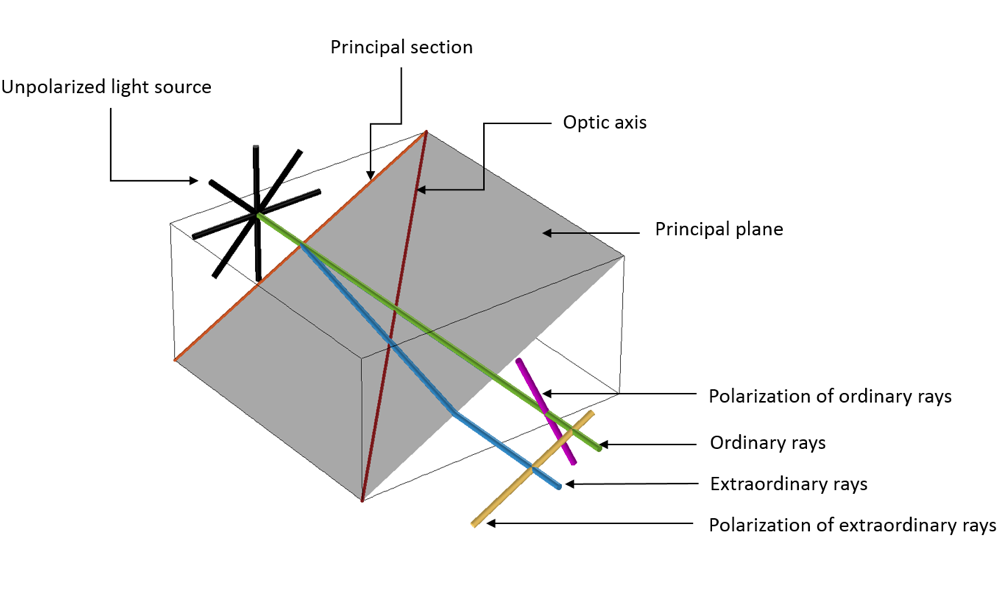
\includegraphics[width=0.6\linewidth]{images/calcite1}\quad
	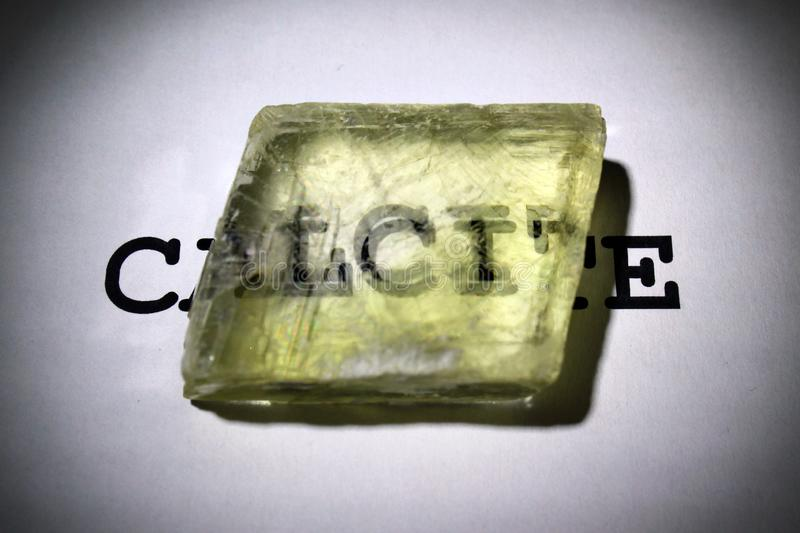
\includegraphics[width=0.4\linewidth]{images/calcite2}
	\caption{Schema ed immagine della rifrazione della luce nella calcite, un dielettrico anisotropo con due assi ottici.}
	\label{fig:calcite1}
\end{figure}
\FloatBarrier
\subsection{Deduzione della legge di Snell (rifrazione)}
Abbiamo notato precedentemente che, essendo la circuitazione di E nulla, la componente tangente si conserva e abbiamo dimostrato che la discontinuità della componente normale è $\frac{\sigma}{\varepsilon_0}$. Consideriamo un campo elettromagnetico che attraversa una superficie sotto la quale è presente un materiale di costante dielettrica relativa \(k_1\) e sopra la quale una costante dielettrica relativa \(k_2\). Conoscendo la direzione della linea di campo entrante nella superficie, per conoscere la direzione della linea di campo uscente dovremmo conoscere $\sigma$, per sapere di quanto cambia la componente normale. Consideriamo una superficie cilindrica di area di base dA e altezza dh che attraversa la superficie perpendicolarmente, siano i vettori normali alle superfici di base \(d\mathbf{s}_1\) e d\(\mathbf{s}_2\). Calcolando il flusso del vettore spostamento elettrico otteniamo
\[\oint_{\Sigma}\mathbf{D}d\mathbf{s} = Q_l = 0\]
poiché nei dielettrici non ci sono cariche libere. Da cui segue
\[D_1ds_1\cos\theta_1 + D_2ds_2\cos\theta_2 = 0\]
Ma \(ds_1 = -ds_2\) quindi chiamando \(D_n\) la componente normale di D
\[D_{n1} = D_{n2}\]
cioè la componente normale di D si conserva, come quella tangente di E, nell'attraversare la superficie che connette un dielettrico ad un altro. Possiamo dunque ricavare $\mathbf{E_2}$
\begin{align*}
	\begin{cases}
		E_1\sin\theta_1 &= E_2\sin\theta_2 \\
		D_1\cos\theta_1 &= D_2\cos\theta_2 
	\end{cases}
\\
	\begin{cases}
		E_1\sin\theta_1 &= E_2\sin\theta_2 \\
		\varepsilon_0k_1E_1\cos\theta_1 &= \varepsilon_0k_2E_2\cos\theta_2 
	\end{cases}
\\
	\Rightarrow \frac{\tan\theta_1}{\tan\theta_2} = \frac{k_1}{k_2}
\end{align*}
Ecco trovata una relazione che permette di trovare il nuovo angolo con cui esce la linea di campo dalla superficie. Essendo la luce un'onda elettromagnetica, anch'essa viene piegata nel passare da un mezzo ad un altro, questo fenomeno è comunemente detto rifrazione e l'ultima relazione ottenuta è la \textbf{legge di Snell}, ottenuta da Willebrord Snell (1580-1626) in modo sperimentale, molto prima della scoperta del campo elettrico e tutto ciò ad esso relativo. Tutte le leggi dell'ottica si ricavano a partire dalle leggi dell'elettromagnetismo. 
\subsection{Energia di un condensatore piano con dielettrico}
Consideriamo un condensatore piano a facce parallele dove lo spazio fra le armature è riempito da un dielettrico di costante dielettrica relativa k e la distanza fra le armature vale d. Sappiamo che
\[C_k = \frac{k\varepsilon_0 S}{d} = \frac{\varepsilon S}{d}\]
\[E_k = \frac{E}{k} = \frac{\sigma}{k\varepsilon_0} = \frac{\sigma}{\varepsilon}\]
Possiamo quindi ricavare l'energia immagazzinata nel condensatore come
\[U = \frac{1}{2}\frac{Q^2}{C_k} = \frac{1}{2}\frac{S^2\sigma^2 d}{\varepsilon S}\frac{\varepsilon}{\varepsilon} = \frac{1}{2}\frac{\sigma^2\varepsilon S d}{\varepsilon^2} = \frac{1}{2}E_k^2\varepsilon V\]
dividendo per il volume si ottiene la densità di energia di un condensatore
\[u = \frac{1}{2}E_k^2\varepsilon  = \frac{1}{2}E_k^2\varepsilon_0 k\]
Si noti che la differenza di energia fra un condensatore con in mezzo un dielettrico e quella con in mezzo il vuoto è data dalla polarizzazione del dielettrico: quando si polarizza il dielettrico non si fa altro che effettuare lavoro per "tirare" ed allontanare i centri di carica degli atomi, passando ad uno stato ad energia potenziale maggiore. La densità di energia necessaria a polarizzare un dielettrico è quindi espressa dalla differenza fra la densità di energia di un condensatore con in mezzo un dielettrico e quella con in mezzo il vuoto
\[\Delta u_p = u_k-u_0 = \frac{1}{2}\varepsilon_0 kE_k^2-\frac{1}{2}\varepsilon_0 E^2 = \frac{1}{2}\varepsilon_0 E^2(\frac{1}{k}-1)<0 \]
La densità è negativa perché il sistema costituito dal dielettrico, nel polarizzarsi, assorbe energia.\\
Nel caso più generale del dielettrico anisotropo si ha 
\[u = \frac{1}{2}\varepsilon_0 \mathbf{k} \mathbf{E} \mathbf{E}(\frac{1}{k}-1) =\frac{1}{2} \mathbf{D} \mathbf{E}\]
dove $\mathbf{k}$ è una matrice 3x3 che moltiplicata al primo $\mathbf{E}$ risulta nel vettore $\mathbf{D}$ che moltiplicato al secondo $\mathbf{E}$ da uno scalare.
\section{Corrente elettrica}
I conduttori sono tali in virtù della presenza di portatori di carica, questi possono essere positivi (protoni) o, come succede più frequentemente, negativi (elettroni). Ad esempio la densità di portatori di carica di rame e argento è
\[N_{Cu} = 8.5 \cdot 10^{28}\frac{e^-}{m^3}\]
\[N_{Ag} = 5.9\cdot 10^{28}\frac{e^-}{m^3}\]
Come si muovono i portatori di carica quando esiste un campo all'interno di un conduttore? Per saperlo è necessario avere uno strumento capace di generare un tale campo, questo è la pila, inventata da Alessandro Volta nel 1799 (prima di questa data uno studio sistematico di questi fenomeni era impossibile). La pila è un generatore di \textbf{forza elettromotrice} (che non è una forza) che intuitivamente è un qualcosa che genera movimento di elettroni.
\begin{definizione}[Forza elettromotrice]
	Si definisce forza elettromotrice \(\varepsilon\) (f.e.m.) di un generatore di corrente l'energia potenziale fornita per unità di carica, cioè il lavoro fatto sull'unità di carica
	\[\varepsilon \equiv \frac{dL}{dQ}\]
\end{definizione}
I portatori di carica si muovono solamente per agitazione termica in assenza di una f.e.m. quindi la media vettoriale delle velocità per agitazione termica è nulla
\[\mathbf{\overline{v}}_0= \sum_{i = 1}^{N}\frac{\mathbf{v}_i}{N}=0\]
Quando attacchiamo la pila si ha una forza sui portatori di carica che quindi sono accelerati; la velocità media non sarà più nulla
\[\mathbf{F}= \pm q\mathbf{E}= m \mathbf{a}\]
Se il campo è costante lungo il conduttore (quando si parla di conduttori possiamo immaginare, per fissare le idee, un filo conduttore), L'accelerazione è costante e il moto è uniformemente accelerato. Ciò vuol dire che le cariche, accelerate per un tempo sufficiente, possono raggiungere velocità infinita (o anche solamente raggiungere la velocità della luce)? Chiaramente no perché all'interno di un conduttore i portatori di carica nel muoversi urtano con il reticolo del conduttore deviando la propria traiettoria e quindi, in media, rallentando; si raggiungerà quindi una velocità di soglia in cui l' accelerazione elettrica e la decelerazione a causa degli urti si bilanciano. \'E evidente un'analogia con l'attrito viscoso
\[\mathbf{F} = \pm q\mathbf{E}-\eta\mathbf{v}=m\mathbf{a}\]
\[\pm q\mathbf{E}=\eta\mathbf{v}_{soglia} \Leftrightarrow \mathbf{a}= 0\]
La costante che compare in questo caso (e che nel caso dell'attrito viscoso è la viscosità) in questo caso è la \textbf{resistività}, il concetto è lo stesso ma in questo caso è dal punto di vista microscopico. Hanno resistività nulla solamente il vuoto e i superconduttori, nei quali è possibile far raggiungere ai portatori di carica velocità prossime a quelle della luce (a causa di effetti relativistici). La velocità dei portatori di carica in modulo è ricavabile dalla teoria cinetica dei gas come valor medio della distribuzione di Maxwell-Boltzmann
\[\overline{v}_0=\sqrt{\frac{3k_b T}{m}}\]
i valori ottenuti da questa formula sono sottostimati di un fattore 10, di cui è possibile render conto solo introducendo la teoria quantistica (teoria di Fermi-Sommerfield).\\
Se è presente un campo nel conduttore (e quindi una f.e.m.) esisterà una velocità media di deriva delle cariche (le possiamo immaginare come una nuvola di portatori di carica che si muove disordinatamente e che trasla in una direzione). Vogliamo ricavare un'espressione della velocità di deriva; consideriamo un conduttore cilindrico con densità di portatori di carica N, all'interno del quale è presente un portatore di carica positivo (in modo da avere lo spostamento equiverso al campo). Consideriamo una superficie \(\Sigma\) che taglia il conduttore trasversalmente, sia $\Delta q$ la carica che attraversa $\Sigma$ nel tempo $\Delta t$
\begin{definizione}[Intensità di corrente]
	Definiamo l'intensità di corrente elettrica come
	\[i \equiv \lim_{\Delta t \to 0} \frac{\Delta q}{\Delta t}=\frac{dq}{dt}\]
	L'unità di misura è l'Ampere
	\[1 A = \frac{1 C}{1 s}\]
\end{definizione}
Quanta carica passa per \(d\mathbf{s}\) (porzione infinitesima di $\Sigma$) in un intervallo di tempo $\Delta t$? Se i portatori di carica hanno una velocità di deriva \(v_d\), quelli che passano $\Sigma$ in $\Delta t$ sono quelli contenuti nel volume di conduttore di base \(ds\cos\theta\) (la superficie $\Sigma$ è inclinata) e altezza $v_d\Delta t$, conoscendo la densità di portatori di carica, essendo i portatori di carica positivi solitamente i protoni, si ha che la densità di carica è \(\rho = N e^+\). Se $\Delta t \to 0$
\[dq = N e^+ d\tau = N e^+ v_d dt ds cos\theta\]

\[di = N e^+ v_d ds cos\theta = N e^+ \mathbf{v}_d\cdot d\mathbf{s}\]
Definiamo il vettore \textbf{densità di corrente}
\[\mathbf{J} \equiv N e^+ \mathbf{v}_d\]
\[di = \mathbf{J}d\mathbf{s}\]
\[i = \int_{\Sigma} \mathbf{J}d\mathbf{s}\]
L'intensità di corrente è quindi il flusso del vettore densità di corrente sulla superficie. Qualora i portatori di carica fossero negativi, in J cambiano segno sia la carica (\(e^-\)) che la velocità quindi J rimane invariato; si ha sempre, indipendentemente dal tipo di portatore, \(\mathbf{J}\) // $\mathbf{E}$. Vediamo che è arbitrario assumere portatori positivi o negativi nella definizione dell'intensità di corrente, essendo più intuitivo il fatto che i portatori siano equiversi al campo scegliamo portatori di carica sempre positivi; ne segue che in un circuito immagineremo sempre portatori di carica che vanno dal punto a potenziale maggiore a quello minore ma nella realtà non è detto che ciò avvenga (anzi, è più frequente che i portatori siano negativi, come in tutti i conduttori). \\
Consideriamo ora una superficie chiusa $\Sigma$ in presenza di un campo vettoriale di densità di carica $\mathbf{J}$ che la attraversa; calcoliamone l'intensità di corrente
\[\oint_\Sigma \mathbf{J}d\mathbf{s} = -\frac{dq}{dt}\]
Intuitivamente, il segno meno deriva dal fatto che se l'intensità di corrente è positiva esce più carica di quanta ne entra quindi la carica interna è diminuita (derivata negativa). Essendo $\Sigma$ una superficie chiusa il vettore normale è sempre uscente, il prodotto scalare fra J e ds sarà quindi positivo quando J esce dalla superficie ($\theta<90^\circ$), negativo quando entra ($\theta>90^\circ$) e nullo quando è perpendicolare (i versi delle disuguaglianze cambiano a seconda del segno del portatore di carica).\\
L'aver aggiunto il segno meno all'integrale chiuso non deriva da considerazioni matematiche ma puramente fisiche (suffragato dall'esperienza), ne deriva dunque un principio (non dimostrabile) dell'elettrodinamica, il \textbf{principio della continuità della carica} o \textbf{legge di conservazione della carica elettrica}:\\
\textit{Il flusso della densità di corrente elettrica attraverso una qualunque superficie chiusa è pari alla variazione della carica elettrica situata nel volume racchiuso dalla superficie nell'unità di tempo.}\\
Possiamo applicare la legge di Gauss per ottenere
\[\oint_\Sigma \mathbf{J}d\mathbf{s} = \int_{V(\Sigma)} \mathbf{\nabla}\mathbf{J} d\tau\]
d'altra parte possiamo esprimere la carica dq come l'integrale di \(d\rho\) in un volume infinitesimo \(d\tau\) 
\[\oint_\Sigma \mathbf{J}d\mathbf{s} = -\int_{V(\Sigma)}\frac{d\rho}{dt}d\tau\]
Eguagliando le due precedenti si ottiene la forma differenziale del teorema di Gauss
\[\mathbf{\nabla}\mathbf{J} = -\frac{d\rho}{dt}\]
Nel caso stazionario (quello più comune, che solitamente considereremo) I è lo stesso in tutti i punti del conduttore ed è costante, che equivale a dire che nonostante vi sia un movimento delle cariche, la quantità di queste al'interno della superficie chiusa è sempre la stessa. Ne segue che in questo caso particolare 
\[\oint_\Sigma \mathbf{J}d\mathbf{s} = -\frac{dq}{dt} = 0\]
\section{Le leggi di Ohm}
Vogliamo ricavare la relazione che lega J ad E. Storicamente quanto andremo a ricavare per via teorica è stato inizialmente osservato sperimentalmente e dall'esperienza se ne sono dedotte le leggi empiriche (macroscopiche); ciò avvenne nella prima metà dell'ottocento. Solo agli inizi del novecento si formulò un modello teorico che rendesse conto dell'esperienza; in particolare le leggi di Ohm sono del 1827 mentre il modello teorico di Grunde-Lorentz è del 1906. Questo modello parte da due considerazioni e due principi:
\begin{itemize}
	\item[C1] Gli elettroni si muovono per agitazione termica (in modo isotropo)
	\item[C2] Essendo il tempo fra due urti molto piccolo i tratti percorsi dagli elettroni fra due urti sono approssimabili a rettilinei (moto uniformemente accelerato)
	\item[P1] Il tempo medio fra due urti non dipende dalla velocità di deriva
	\item[P2] Dopo un urto la distribuzione di velocità è isotropa
\end{itemize}
Soffermiamoci sui due principi: il primo è equivalente a dire che la velocità di deriva è trascurabile rispetto a quella di agitazione termica, questo è valido a temperature "normali" ma in alcuni casi, ad esempio a basse temperature e con materiali poco resistivi e con alte differenze di potenziale ciò può non essere vero e il modello perde di validità; il secondo invece ci dice che nell'istante successivo ad un urto la velocità dipende solamente dall'agitazione termica perché ancora il campo elettrico non ha avuto il tempo di accelerare l'elettrone in una direzione, essendo la velocità di agitazione termica isotropa, anche la velocità a seguito di un urto è isotropa (nel tempo la velocità dovuta al campo aumenta e si crea una direzione privilegiata in cui la velocità è maggiore e dunque smette di essere isotropa). I materiali che soddisfano questi due principi sono detti ohmici.\\
Sia \(v_{i+1}\) la velocità subito prima di un urto, \(v_i\) quella subito dopo e $\overline{t}$ il tempo medio fra due urti essendo il moto uniformemente accelerato, la velocità prima dell'urto è uguale alla velocità iniziale (isotropa, dovuta all'agitazione termica) più l'accelerazione dovuta al campo per il tempo medio fra due urti
\[\mathbf{v}_{i+1}  = \mathbf{v}_i - \frac{e\mathbf{E}}{m_e}\overline{t}\]
\[\mathbf{v}_d = \sum_i\frac{\mathbf{v}_{i+1}}{N}= \frac{\sum_i\mathbf{v}_i}{N} - \frac{e\mathbf{E}}{m_e}\overline{t} \frac{N}{N} = - \frac{e\mathbf{E}}{m_e}\overline{t}\]
dove il primo addendo si elimina perché la media vettoriale di una velocità isotropa è nulla. Possiamo riscrivere il vettore di densità di corrente
\[\mathbf{J}= Ne\mathbf{v_d}= \frac{Ne^2\overline{t}\mathbf{E}}{m_e}\]
Definiamo la \textbf{conduttività} $\sigma'$ e la \textbf{resistività} $\rho'$
\[\sigma' \equiv \frac{Ne^2\overline{t}}{m_e}\]
\[\rho' \equiv \frac{1}{\sigma'}= \frac{m_e}{Ne^2\overline{t}}\]
osserviamo che il tempo medio fra due urti dipende dal passo del reticolo cristallino l e dalla velocità di agitazione termica (\(\overline{t}= \frac{l}{v_i}\)), ne segue che conduttività e resistività dipendono solo dal tipo di materiale (in N ed l) e dalla temperatura ( in $\mathbf{v}_i$). \\
In conclusione
\[\mathbf{E}= \rho' \mathbf{J}\]
\[\mathbf{J}= \sigma' \mathbf{E}\]
Queste sono forme equivalenti alle leggi di Ohm, che possiamo ricavare semplicemente.\\
Si consideri un circuito in condizioni stazionarie (I costante) e con campo elettrico costante con differenza di potenziale \(\Delta V_{AB}\) a cui è collegato un cilindro di materiale conduttore di altezza l e superficie di base S. 
\[\Delta V = \int_{A}^{B}\mathbf{E}d\mathbf{l}=El\]
\[i = \int_S \mathbf{J}d\mathbf{s}= JS= \frac{E S}{\rho}\]
\[\Rightarrow E = \frac{\rho'}{S}i\]
\[\Rightarrow \Delta V = \frac{l\rho'}{S}i \equiv R i\]
dove R è la \textbf{resistenza}. Quest'ultima è la prima legge di Ohm, la seconda è proprio la definizione di resistenza R
\[R \equiv \frac{\rho' l}{S}\]
\begin{definizione}[Resistenza]
Proprietà di un circuito elettrico o di parte di esso che trasforma energia elettrica in calore, opponendosi al passaggio di corrente elettrica. Spesso considerata in un punto localizzato del circuito, è in realtà caratteristica di ogni parte di esso. Viene rappresentata con il simbolo
\begin{figure}[h!]
	\centering
	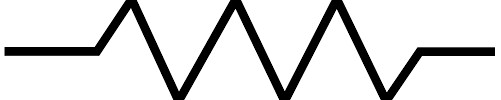
\includegraphics[width=0.3\linewidth]{images/resistenza}
	\caption{Simbolo della resistenza elettrica.}
	\label{fig:resistenza}
\end{figure}
\FloatBarrier
\end{definizione}
\subsection{Resistenze in serie e in parallelo}
Consideriamo due resistenze uguali collegate in serie come in figura
\begin{figure}[h!]
	\centering
	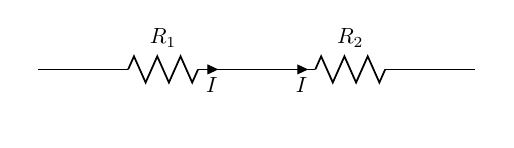
\includegraphics[width=0.6\linewidth]{images/resistenze_serie}
	\caption{Resistenze in serie}
	\label{fig:resistenzeserie}
\end{figure}
\FloatBarrier
Intuitivamente, ci aspettiamo che la resistenza totale aumenti a causa dell'aumentare della lunghezza totale della resistenza. Considerando il circuito diviso dalle due resistenze nelle parti A, B, C, possiamo esprimere la differenza di potenziale in due modi differenti e poi uguagliare
\[\Delta V = V_a - V_c = R_{tot}i\]
\[\Delta V = V_a -V_b + V_b- V_c = (R_1 + R_2)i\]
\[\Rightarrow R_tot = R_1 + R_2\]
che può essere esteso al caso di n resistenze in serie e al caso continuo come segue
\[R_{tot} = \sum_{i=1}^N R_i \]
\[R_{tot} = \int dR\]
Ne deduciamo che, avendo una resistenza di forma irregolare, possiamo considerare ogni sezione trasversale come una resistenza collegata in serie con le altre ed integrare come segue
\[R_{tot}= \int_{a}^{b}\frac{\rho'}{S(l)}dl\]
Nelle resistenze in parallelo invece, intuitivamente, aumenta la superficie attraverso cui può passare la corrente e quindi ci aspettiamo una diminuzione della corrente. Consideriamo due resistenze in parallelo come in figura
\begin{figure}[h!]
	\centering
	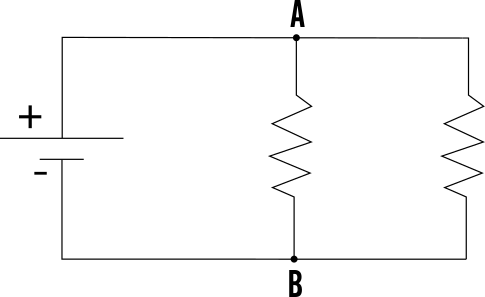
\includegraphics[width=0.5\linewidth]{images/resistenze_parallelo}
	\caption{Schema di due resistenze in parallelo}
	\label{fig:resistenzeparallelo}
\end{figure}
\FloatBarrier
\[\Delta V = R_1i_1= R_2i_2\]
\[i = i_1+i_2\]
\[i_1 = \frac{\Delta V}{R_1}\quad i_2 = \frac{\Delta V}{R_2} \]
\[ i = \Delta V \left(\frac{1}{R_1}+\frac{1}{R_2}\right)= \frac{\Delta V}{R_{tot}} \]
\[\Rightarrow \frac{1}{R_{tot}} = \frac{1}{R_1}+\frac{1}{R_2} \]
Che si estende a 
\[\frac{1}{R_{tot}}= \sum_{i = 1}^N\frac{1}{R_i}\]

\subsection{Resistenze dal punto di vista energetico: effetto Joule}
In presenza di campo elettrico gli elettroni hanno una velocità di deriva, se spengo il campo tornano ad avere velocità media nulla, qual'è la potenza che devo erogare per mantenere costante questa velocità (e quindi sconfiggere oppormi alla resistenza)? Cominciamo considerando quella necessaria ad un singolo portatore di carica
\[P_i = \frac{dL}{dt}= \frac{\mathbf{F}\mathbf{dr}}{dt}= \mathbf{F}\mathbf{v_d}= -q\mathbf{E}\mathbf{v_d}\] 
moltiplicando per la densità di portatori di carica otteniamo la densità volumetrica di potenza necessaria, osservando che la carica di un portatore coincide con quella dell'elettrone otteniamo
\[\frac{P}{V}= nP_i=  (-ne\mathbf{v_d})\mathbf{E}= \mathbf{J}\mathbf{E}= \sigma' E^2= \rho' J^2\]
quest'ultima è una versione della \textbf{legge di Joule}, essa esprime la quantità di energia dissipata per unità di tempo e volume in un conduttore. Per ottenere la forma più conosciuta ed utile nelle applicazioni, consideriamo un conduttore cilindrico di sezione S e lunghezza l
\[P = (Sl) \rho' J^2 \frac{S}{S} = \frac{\rho' l}{S}(J^2 S^2)= Ri^2= \Delta V i \]
Microscopicamente, l'energia viene dissipata a causa degli urti dei portatori di carica che generano calore, ovvero energia che viene dissipata; macroscopicamente osserviamo che il conduttore si riscalda a causa del passaggio di corrente. Si osservi che all'aumentare della temperatura la resistenza aumenta, ne segue che aumenta la potenza dissipata e quindi la temperatura, ricomincia così il circolo vizioso che potrebbe portare a temperature altissime; ciò spiega perché è fondamentale la refrigerazione di impianti e dispositivi elettrici come i computer (che rischierebbero di fondere).    
\section{Generatori}
Tutti i circuiti visti fin ora presuppongono l'esistenza di un generatore che mantenga costante la \(\Delta V\) fra i capi del circuito. Consideriamo la differenza di potenziale tra i capi di un filo conduttore, mantenuta costante da un generatore
\[\Delta V = \int_a^b \mathbf{E_{el}}\mathbf{dr}= Ri\]
Sappiamo che la circuitazione del campo elettrostatico è nulla, in un circuito in cui si considerano portatori di carica in movimento si deve tener conto anche delle resistenze quindi all'interno del circuito (da A a B) la differenza di potenziale non può essere nulla. La restante parte di circuito da considerare per ottenere la circuitazione è quello che va da B ad A, ovvero la parte di circuito interna al generatore. Sia \(\mathbf{E^*}\) il campo prodotto dal generatore, al suo interno è presente in totale il campo \(\mathbf{E^*}+\mathbf{E_{el}}\) mentre nel resto del circuito c'è solo \(\mathbf{E_{el}}\) a priori vi sono le seguenti possibilità:
\begin{itemize}
	\item \(\mathbf{E^*} \geq 0\) o \((\mathbf{E^*} < 0) \wedge (|{E^*}| \leq |{E_{el}}|)\) Questi casi sono impossibili, violano il primo principio della termodinamica.
	\item \(\mathbf{E^*} < 0\),  \(|{E^*}| > |{E_{el}}|\) In questo caso all'interno del generatore il campo totale è negativo, in questo modo si genera una differenza di potenziale fra i punti AB che permette l'esistenza di una corrente elettrica. 
\end{itemize}
La f.e.m. di un circuito siffatto è 
\[\oint_{\Gamma}\mathbf{E_{tot}}\mathbf{dl}= \int_{a}^{b}\mathbf{E_{el}}\mathbf{dl}+\int_{b}^{a}\mathbf{E^*}+\mathbf{E_{el}}\mathbf{dl}= Ri + R_{gen}i\]
dove la prima resistenza è quella offerta dal conduttore mentre la seconda quella offerta dal generatore. Possiamo vedere lo stesso calcolo in modo diverso come
\[\oint_{\Gamma}\mathbf{E_{tot}}\mathbf{dl}= \int_{a}^{b}\mathbf{E_{el}}\mathbf{dl} + \int_{b}^{a}\mathbf{E^*}\mathbf{dl} +  \int_{b}^{a}\mathbf{E_{el}}\mathbf{dl}= \int_{b}^{a}\mathbf{E^*}\mathbf{dl}\]
\[\Rightarrow \varepsilon = \oint_{\Gamma}\mathbf{E_{tot}}\mathbf{dl} = \int_{b}^{a}\mathbf{E^*}\mathbf{dl} = (R + R_{gen})i \]
ne segue che possiamo trattare un generatore come un pezzo di circuito che offre una sua resistenza \(R_{gen}\). \(\mathbf{E^*}\) è detto \textbf{campo elementare} e non è conservativo, infatti è proprio l'unica componente di circuitazione non nulla. Possiamo ricavare le seguenti relazioni
\begin{align*}
	&i = \frac{\varepsilon}{R+R_{gen}}\\
	&\Delta V = \varepsilon-R_{gen}i
\end{align*}
Ne deduciamo che la differenza di potenziale che effettivamente è prodotta da un generatore è minore della f.e.m. indotta da questo. Nelle comuni pile è indicata la f.ew.m. e non la $\Delta V$.\\
Da un punto di vista energetico, la potenza totale dissipata da un circuito con generatore
\[P = \varepsilon_i = R i^2 + R_{gen}i^2\]
La potenza non è quindi dissipata solo dall'effetto Joule del conduttore ma anche da quello del generatore. 
\section{Circuiti in regime quasi stazionario: il circuito RC}
Fin ora, parlando di resistenze, abbiamo considerato solamente circuiti in cui la corrente è costante in tutti i punti del circuito, l'unico caso diverso che considereremo è il regime stazionario. Consideriamo un circuito con un condensatore, un generatore, un interruttore ed una resistenza in serie (detto circuito RC), a circuito aperto non vi è corrente e il condensatore è scarico, quando si chiude il circuito, dopo un tempo sufficientemente lungo si raggiunge una situazione di equilibrio; vogliamo sapere come evolva il sistema in questo periodo (in particolare le espressioni di q(t) e i(t)). 
\begin{figure}[h!]
	\centering
	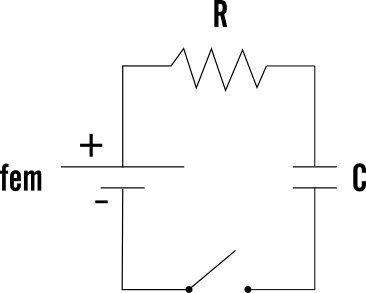
\includegraphics[width=0.6\linewidth]{images/circuito-rc}
	\caption{Schema del circuito RC.}
	\label{fig:circuito-rc}
\end{figure}
\FloatBarrier
Per ottenere q(t) impostiamo una equazione differenziale a partire dall'espressione della f.e.m.. Considerando la resistenza interna al generatore trascurabile, otteniamo da una relazione vista in precedenza 
\[\varepsilon = \Delta V = \Delta V_{ab} + \Delta_{bd} = \frac{q(t)}{C}+R\frac{dq(t)}{dt}\]
Otteniamo quindi l'equazione differenziale del primo grado, risolvibile con il metodo di separazione delle variabili
\[\Delta V-q = RC \dot{q}\]
\[\frac{dq}{q-C\Delta V}= -\frac{dt}{RC}\]
\[q(t) = -e^{-\frac{t}{RC}}C\Delta V+C\Delta V = C\Delta V(1-e^{-\frac{t}{RC}})\]
\[i(t) = \frac{dq}{dt} = \frac{\Delta V}{R}e^{-\frac{t}{RC}}\]
\[\Delta V_{ab}(t)=\frac{q}{C}= \Delta V(1-e^{-\frac{t}{RC}})\]
\[\Delta V_{bd}(t)=Ri(t)= \Delta Ve^{-\frac{t}{RC}}\]
Osserviamo come la funzione q(t) tenda asintoticamente al valore \(Q=C\Delta V \), ciò vuol dire che il condensatore è sempre in carica ma, essendo la funzione esponenziale, già dopo pochissimo sarà carico quasi del tutto e la corrente che passa nel circuito per completare la carica è minima. Possiamo avere un'idea del tempo che impiega un condensatore a caricarsi alla percentuale p come segue
\[\frac{Q-q(t)}{Q} = e^{-\frac{t}{RC}}=p\]
L'unica incognita è il tempo; per una carica del 99.9\%,99\%,95\% deve passare rispettivamente un tempo di 7RC, 4.6RC,3RC. Notiamo che l'unità di misura di RC è proprio un tempo, che è caratteristico dello specifico circuito, viene infatti detto \textbf{tempo proprio del circuito}. Un valore tipico di tempo proprio è di \(1\mu s \), per caricare al 99.9\% un condensatore servono dunque \(7\cdot10^{-6}\ s\). \\
Dal punto di vista energetico, una parte di energia per caricare il condensatore è dissipata durante il processo di carica per effetto Joule. Calcoliamo l'energia che il generatore immette nel sistema per caricare completamente il condensatore integrando l'espressione della potenza erogata in un tempo infinito (abbiamo visto che la carica è un processo infinito). 
\[L_{gen} = \int_{0}^{+\infty}P_{gen}(t)dt=\int_{0}^{+\infty}\Delta V i(t)dt = \int_{0}^{+\infty}\frac{\Delta V^2}{R} e^{-\frac{t}{RC}}dt = C\Delta V^2 \]
Ne deduciamo che L'energia fornita dal generatore per caricare il condensatore è doppia rispetto a quella immagazzinata da questo una volta carico (\(U=\frac{1}{2}X\Delta V^2\)), l'altra metà è persa per effetto Joule. Possiamo pervenire allo stesso risultato integrando la potenza dissipata per effetto Joule in un tempo infinito per ottenere l'energia dissipata nel processo di carica. 
\[L_{R} = \int_{0}^{+\infty}P_{R}(t)dt =\int_{0}^{+\infty}Ri(t)^2dt = \int_{0}^{+\infty}\frac{\Delta V^2}{R}e^{-\frac{2t}{RC}}dt = \frac{1}{2}C\Delta^2\]
\section{Il magnetismo}
\subsection{Evidenze sperimentali}
A partire dalla prima metà dell'Ottocento, grazie all'avanzamento della tecnica, studiosi quali Coulomb (1736-1806), Ampere (1775-1836), \O{}rsted (1777-1851) Faraday (1791-1867), Lorentz (1853-1928)
Coulomb sperimentalmente pervenne ad una legge simile a quella ottenuta per la forza generata da un campo elettrico, ipotizzando così l'esistenza di "cariche magnetiche" positive e negative simili a quelle elettriche, spinto anche dall'analogia nella forma delle tre forze naturali che sembravano poter descrivere tutti i fenomeni conosciuti (gravità, elettricità e magnetismo). 
\[\mathbf{F}=k\frac{q_{m1}q_{m_2}}{r^2}\mathbf{\hat{r}}\]
Alla forza magnetica, in analogia con quanto visto per quella elettrica, possiamo associare un campo magnetico, indicato dalla lettera $\mathbf{B}$; la sua unità di misura è il Tesla (\(T\)) nel S.I. e il Gauss nel C.G.S. Il Tesla è un' unità di misura molto grande e si usano spesso suoi sottomultipli
\[1G=10^{-4}T\]
Il problema che rende l'approccio di Coulomb sostanzialmente sbagliato è che si verifica sperimentalmente che è impossibile isolare cariche magnetiche positive e negative; avendo un magnete superiormente carico negativamente e inferiormente positivamente, una volta spezzato in due parti produce due nuovi magneti con le stesse caratteristiche.
\begin{figure}[h!]
	\centering
	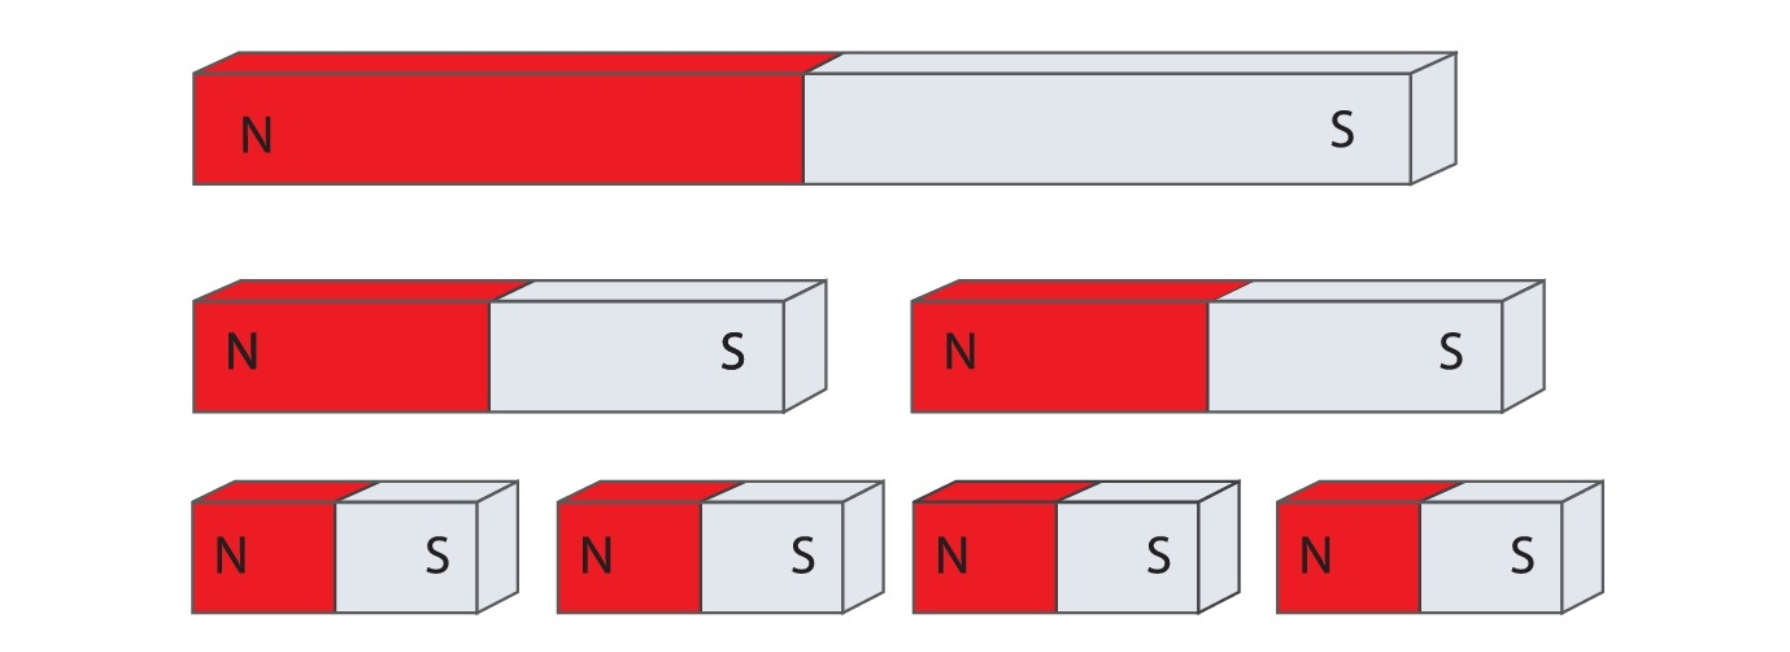
\includegraphics[width=0.5\linewidth]{images/magnete_rotto}
	\caption{Si osserva l'impossibilità sperimentale di ottenere "monopoli magnetici" per scissione di un magnete.}
	\label{fig:magneterotto}
\end{figure}
\FloatBarrier
\'{E} interessante che in tempi recenti sono stati condotti esperimenti (basati su teorie moderne) che ricercavano l'esistenza di monopoli magnetici, finora mai osservati.\\
Ciò rende i fenomeni magnetici diversi da quelli elettrici perché le linee di forza di un campo magnetico sono sempre necessariamente chiuse, perché partendo da un polo, rientrano sempre al polo di carica opposta. Ne segue che il campo magnetico ha sempre flusso nullo
\[\Phi(\mathbf{B}) = 0\] 
In seguito alcuni esperimenti misero in luce le strette relazioni tra campo magnetico ed elettrico. L'esperimento di \O{}rsted mette in luce il fatto che un filo attraversato da corrente fa ruotare un'ago magnetico (dunque produce campo magnetico) orientandolo perpendicolarmente alla direzione del flusso di corrente elettrica; deduce inoltre che il campo prodotto dal filo è circolare, ortogonale ad esso e di verso che segue la regola della mano destra. Ampere osserva che anche tra due fili attraversati da corrente si genera una forza (che ipotizza di tipo magnetico) attrattiva se direzione e verso della corrente sono paralleli e concordi, repulsiva se paralleli e discordi. Infine Faraday osserva che un filo attraversato da corrente posto ortogonalmente fra due poli di un magnete sperimenta una forza ortogonale sia al filo che all'asse congiungente i due poli.\\
\subsection{Deduzioni dai fatti sperimentali}
Da queste leggi deduciamo che la Forza generata dal campo magnetico deriva da un prodotto scalare (risulta ortogonale ai due agenti che sembrano provocarla: il campo magnetico e la corrente elettrica), l'ordine dei fattori si deduce dall'orientamento della forza risultante e si osserva, seguendo il principio della mano destra, che il primo è legato alla direzione della corrente e il secondo dal campi magnetico. Tuttavia bisogna notare che per come è stata definita la corrente è uno scalare, è dunque errato parlare di "direzione della corrente", in realtà la direzione è quella del vettore velocità degli elettroni che attraversano il filo, la corrente è in relazione diretta sia con la velocità degli elettroni sia con la quantità di questi (e quindi con la carica in generale). Da queste considerazioni Lorentz formulò l'omonima legge
\[\mathbf{F}=q\mathbf{v}\wedge\mathbf{B}\]
Notiamo subito un'altra differenza con il campo elettrico: la forza è ortogonale alle linee di campo quindi non è indifferente parlare di "linee di campo" o "linee di forza", inoltre questa forza esiste solo se le cariche sono in movimento (il magnetismo infatti non è osservabile nell'ambito dell'elettrostatica). Inoltre, calcolando il lavoro
\[L = \int_a^b \mathbf{F}\mathbf{dl}=\int_a^b (q\mathbf{v}\wedge\mathbf{B})\cdot \mathbf{dl}= \int_a^b (q\mathbf{v}\wedge\mathbf{B})\cdot \mathbf{v}dt= 0 \]
poiché il prodotto vettoriale risulta in un vettore ortogonale ad entrambe i fattori, ed il prodotto scalare fra vettori ortogonali è nullo. Ne segue che il campo magnetico non fa mai lavoro.\\
Per il teorema delle forze vive 
\[L = \frac{1}{2}m(v_f^2-v_i^2) = 0 \]
\[\Rightarrow v_f = v_i\]
Si presti attenzione al fatto che ciò non implica \(\mathbf{v_f} = \mathbf{v_i}\) poiché il campo magnetico non può cambiare il modulo della velocità di un corpo ma può cambiare la sua direzione.\\
Consideriamo una carica di velocità costante $\mathbf{v}$ ortogonale ad un campo magnetico $\mathbf{B}$, il modulo della Forza di Lorentz è
\[F = qvB\]
perpendicolare alla traiettoria (quindi centripeta) e costante. Eguagliando questa espressione a quella della forza centripeta otteniamo
\[qvB=\frac{mv^2}{r}\ \Rightarrow\ r=\frac{mv}{qB}\]
poiché r, il raggio di curvatura, è costante, il moto che ne risulta yz (considerando la velocità della carica in direzione x) è di tipo circolare uniforme. Altre grandezze di interesse possono essere facilmente ricavate
\[\omega=\frac{qB}{m}\]
\[T=\frac{2\pi m }{qB}\]
Se invece la velocità della carica non è ortogonale a $\mathbf{B}$, scomponiamo la velocità nelle componenti perpendicolare e parallela a B \(\mathbf{v}=\mathbf{v_{\perp}}+\mathbf{v_{//}}\)
\[\mathbf{F} = q(\mathbf{v_{\perp}}+\mathbf{v_{//}})\wedge \mathbf{B}=q\mathbf{v_{\perp}}\wedge \mathbf{B}+q\mathbf{v_{//}}\wedge \mathbf{B}= q\mathbf{v_{\perp}}\wedge \mathbf{B} \] 
dove il termine di velocità parallela al campo magnetico si annulla. Ricordando l'espressione generale della forza centripeta in funzione di $\mathbf{\omega}$ ed $\mathbf{r}$
\[\mathbf{F}= q\mathbf{v_{\perp}}\wedge \mathbf{B}= m \mathbf{\omega}\wedge(\mathbf{\omega}\wedge\mathbf{r})= m\mathbf{\omega}\wedge\mathbf{v}= -m\mathbf{v}\wedge\mathbf{\omega} \] 
\[\mathbf{v_{\perp}}\wedge \mathbf{B}= -\frac{m}{q}\mathbf{v}\wedge\mathbf{\omega} =\mathbf{v}\wedge\left(-\frac{m}{q}\mathbf{\omega}\right) \]
\[\Rightarrow \mathbf{\omega}= -\frac{q}{m}\mathbf{B}\]
Ma che moto ha la carica nello spazio? La forza sull'asse x è nulla dunque in questa direzione il moto è rettilineo uniforme con velocità pari a quella costante iniziale. Sul piano yz invece c'è una forza centripeta che produce un moto circolare uniforme.
\[\mathbf{F}= q\mathbf{v}\wedge\mathbf{B}= qvB\sin\theta\]
La composizione di questi due moti è detta \textbf{moto elicoidale}
\begin{figure}[h!]
	\centering
	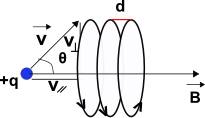
\includegraphics[width=0.5\linewidth]{images/moto_elicoidale}
	\caption{Rappresentazione del moto elicoidale}
	\label{fig:motoelicoidale}
\end{figure}
\FloatBarrier
Nel caso più generale di una carica sottoposta sia a campo elettrico costante che magnetico abbiamo
\[\mathbf{F}= q\mathbf{E}+q\mathbf{v}\wedge\mathbf{B}\]
Fin ora abbiamo considerato la forza di Lorentz su una carica, in un conduttore le cariche si muovono per agitazione termica, che ha somma vettoriale nulla, se vi è applicato un campo magnetico avremo una velocità di deriva risultante che genera anche campo magnetico. La forza di Lorentz in una porzione di filo conduttore di sezione $\Sigma$ e lunghezza dl è
\[\mathbf{dF}=n(\Sigma dl)\mathbf{F_i} = n\Sigma dl q\mathbf{v}\wedge\mathbf{B}= -n\Sigma dl e\mathbf{v}\wedge\mathbf{B} = \Sigma dl \mathbf{J}\wedge\mathbf{B}= i\mathbf{ds}\wedge\mathbf{B}\]  
\[\Rightarrow \mathbf{F}=i\mathbf{l}\wedge\mathbf{B}\]
dove n è la densità dei portatori di carica e \(\mathbf{F_i}\) la forza di Lorentz generata da una singola carica, q è stato sostituito con -e, la carica dell'elettrone, in quanto in un conduttore metallico i portatori di carica sono gli elettroni liberi. Si dimostra che la forza non dipende dal cammino del filo e che $\mathbf{l}$ è in realtà la distanza tra due punti del filo.  
\subsection{Applicazioni}
\begin{applicazione}[Spettrometro di massa]
Basandosi sul fatto che il campo magnetico è legato alla velocità della carica è possibile creare un apparato che selezioni particelle che viaggiano ad una specifica velocità, basandosi poi sul fatto che il campo magnetico genera una forza centripeta che curva il moto delle cariche in base non solo loro velocità ma anche a massa e carica di queste, è possibile ottenere informazioni su queste grandezze se i campi magnetici hanno intensità nota.\\
Inizialmente abbiamo un campione di particelle già cariche o previamente ionizzate, di velocità differenti (ad esempio secondo una distribuzione di Maxwell-Boltzmann), innanzitutto bisogna selezionare le particelle di una specifica velocità con l'utilizzo di un \textbf{selettore di velocità}, costituito da un condensatore all'interno del quale è presente un campo magnetico ortogonale alle facce in modo da produrre una forza di Lorentz  parallela e discorde a quella generata dal campo elettrico. Una carica, supponiamo un elettrone, che passa per questo apparato è sottoposta alle forze (che consideriamo in modulo essendo tutte parallele e verticali)
\[F_{tot} = e\mathbf{E}-(evB_1)\]
Se la forza totale non è nulla gli elettroni saranno deflessi, gli unici a proseguire dritto saranno quelli di velocità \(v_0\) tale che
\[F_{tot}= e\mathbf{E}-(ev_0B_1)=0\]
\[\Rightarrow v_0=\frac{E}{B_1}\]
\begin{figure}[h!]
	\centering
	\includegraphics[width=0.5\linewidth]{images/selettore_velocità}
	\caption{Schema di un selettore di velocità. Il funzionamento è indipendente dal segno della carica del portatore.}
	\label{fig:selettorevelocita}
\end{figure}
\FloatBarrier
Una volta selezionata la velocità vogliamo avere informazioni su carica e massa di queste particelle. Ci avvaliamo di uno strumento come quello in figura (il selettore di velocità non è rappresentato).
\begin{figure}[h!]
	\centering
	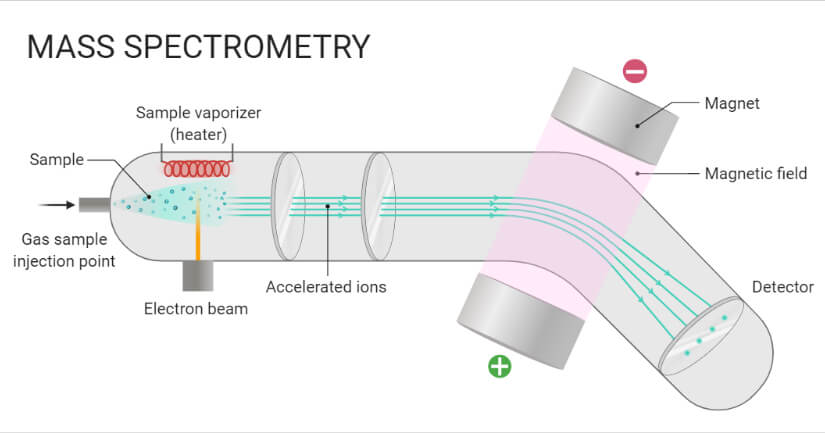
\includegraphics[width=0.7\linewidth]{images/spettrometro}
	\caption{Schema di uno spettrometro di massa}
	\label{fig:spettrometro}
\end{figure}
\FloatBarrier
Innanzitutto la velocità iniziale dovrebbe essere aumentata di un valore noto (mediante campi elettrici) per amplificare le grandezze da misurare, non teniamo conto di questo accorgimento di facile implementazione. In seguito si applica un campo magnetico $\mathbf{B_2}$, la forza di Lorentz, centripeta, vale
\[F = evB_2= \frac{mv_0^2}{R}\]
\[eB_2 = \frac{mv_0}{R}= \frac{mE}{RB_1} \]
\[\Rightarrow \frac{e}{m}= \frac{E}{RB_1B_2}\]
In base al raggio di curvatura R, misurabile mediante un detector posto all'estremità dell'apparato, essendo i campi applicati tutti noti, è possibile ricavare il rapporto carica/massa.
\end{applicazione}
\begin{applicazione}[Effetto Hall]
	Consideriamo un parallelepipedo conduttore di spessore d, larghezza l e lunghezza h, attraversato da un flusso densità di corrente $\mathbf{J}$ e da un campo magnetico \(\mathbf{B}\) ad esso ortogonale
\begin{figure}[h!]
	\centering
	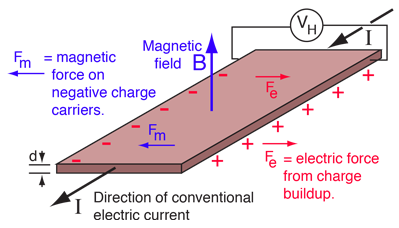
\includegraphics[width=0.6\linewidth]{images/hall_effect}
	\caption{Schema dell'effetto Hall.}
	\label{fig:halleffect}
\end{figure}
\FloatBarrier
Inizialmente il conduttore è neutro, le cariche, di velocità di deriva $\mathbf{v_d}$ sono sottoposte ad una forza di Lorentz che, considerandole di carica negativa, le spinge verso la faccia sinistra (si veda la figura)
\[\mathbf{F}= q\mathbf{v_d}\wedge\mathbf{B}\] 
Possiamo definire il campo di Hall come
\[\mathbf{E_H}=\frac{\mathbf{F}}{q}=\mathbf{v_d}\wedge\mathbf{B}=\frac{\mathbf{J}}{nq}\wedge\mathbf{B}\]
Le cariche negative col tempo si addensano sulla faccia sinistra generando una differenza di potenziale fra le facce e quindi un campo elettrico che si oppone al campo di Hall. Dopo un intervallo di tempo sufficientemente lungo i due campi si annullano e si raggiunge l'equilibrio. Possiamo definire la forza elettromotrice di Hall come
\[\Delta V_H = E_H l =\frac{BJ}{nq}l =\frac{iB}{ldnq}l=\frac{i B}{nqd} = R_H \frac{iB}{d}\] 
dove è stata usata la formula della \(\Delta V\) per i condensatori, ed \(R_H\) è la \textbf{costante di Hall}.
\end{applicazione}
\subsection{Misurare il campo magnetico}
Come già osservato l'ideazione di un'apparato sperimentale per la misura di una grandezza offre la possibilità di dedurne informazioni teoriche. Nel caso del campo magnetico il primo semplice metodo di misura del campo magnetico è basato sullo studio del moto di una spira immersa in un campo magnetico
\begin{definizione}[Spira]
	 In elettrotecnica la spira di un avvolgimento solenoidale è il tratto di conduttore corrispondente a un passo dell’elica di avvolgimento; poiché tale tratto è proporzionale al campo magnetico generato dall'intero avvolgimento percorso da corrente, il termine ha finito con l’essere usato, in elettromagnetismo, per indicare un circuito chiuso, per es. un circuito filiforme circolare (spira circolare) o poligonale (spira rettangolare, quadrata, ecc.).
\end{definizione}
Consideriamo una spira rettangolare di lati a,b attraversata da corrente in senso antiorario. Il circuito individua una superficie S di vettore normale $\mathbf{\hat{u_n}}$ (il verso si determina con la regola della mano destra). Si consideri un campo magnetico $\mathbf{B}$ passante per S che forma un angolo $\theta$ con $\mathbf{\hat{u_n}}$. Le forze che agiscono sui lati del solenoide sono a due a due uguali, 
\begin{figure}[h!]
	\centering
	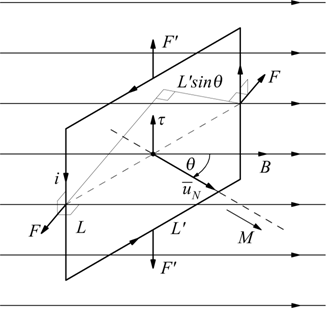
\includegraphics[width=0.5\linewidth]{images/spira_campo_magnetico}
	\caption{Spira immersa in un campo magnetico, le forze sui lati superiore ed inferiore si annullano a vicenda, quelle sui lati destro e sinistro generano momento.}
	\label{fig:spiracampomagnetico}
\end{figure}
\FloatBarrier
La forza di Lorentz totale sulla spira è
\[\mathbf{F}= \int_{\Gamma}dq\mathbf{v}\wedge\mathbf{B}= \int_{\Gamma}dq\frac{\mathbf{ds}}{dt}\wedge\mathbf{B}= i \int_{\Gamma}\mathbf{ds}\wedge\mathbf{B}\]
Possiamo spezzare questo integrale di percorso nei 4 lati, chiamiamo 1 e 3 quelli superiore e inferiore di lunghezza a, 2 e 4 quelli destro e sinistro di lunghezza b.\\
Sui lati superiore e inferiore il campo è ortogonale alla velocità e la forza di Lorentz risulta ortogonale al lato del solenoide, essendo il verso della velocità opposto su questi due lati, le due forze si annullano. Sui lati destro e sinistro invece l'angolo fra il campo magnetico e il vettore velocità è \(2\pi-\theta\) da cui
\[F_1=F_3 = iaB \sin(\frac{\pi}{2}) = iaB \]
\[F_2=F_4 = ibB \sin(2\pi-\theta) = -ibB\sin(\theta) \]
Il momento delle forze sulla spira, prendendo come polo il centro del rettangolo, osservando che il braccio r è uguale per le due forze, pari a metà del lato a, è quindi
\[\mathbf{\tau}= \mathbf{r}\wedge\mathbf{F_2}+\mathbf{r}\wedge\mathbf{F_4}=2(-\frac{ab}{2}i\sin\theta)= -i SB \sin\theta\]
Ricordando l'espressione del momento delle forze in funzione di $\theta$, impostiamo l'equazione differenziale che descrive il moto della spira
\[\mathbf{\tau}=I\ddot{\theta}=- iSB\sin\theta\]
Per piccoli valori di $\theta$ possiamo approssimare $\sin\theta \simeq \theta$, ottenendo l'equazione differenziale armonica: spostando la spira, a partire da una posizione di equilibrio, di un piccolo angolo $\theta$, il campo tende a farla tornare alla posizione iniziale instaurando un moto armonico. 
\[\ddot{\theta}+ \frac{iSB}{I}\theta= 0 \]
Osserviamo che l'espressione di $\mathbf{\tau}$ è esprimibile come prodotto vettoriale
\[\mathbf{\tau}=iS\mathbf{\hat{u}_n}\wedge\mathbf{B}=-iSB\sin\theta\]
Possiamo definire il vettore \textbf{momento magnetico della spira} e sostituire
\[\mathbf{m}\equiv iS\mathbf{\hat{u}_n}\] 
\[\mathbf{\tau}=\mathbf{m}\wedge\mathbf{B}\]
Osserviamo un'analogia fra il momento generato da una spira percorsa da corrente e quello generato da un dipolo elettrico ($\mathbf{\tau}=\mathbf{P}\wedge\mathbf{E}$). A partire da queste considerazioni Ampere formula l'omonimo principio di equivalenza: \textit{una spira attraversata da corrente equivale ad un dipolo magnetico e, più in generale una calamita equivale ad un circuito attraversato da corrente}.\\
Risolvendo l'equazione differenziale otteniamo
\[\omega=\sqrt{\frac{mB}{I}}\]
\[T=2\pi\sqrt{\frac{I}{mB}}\]
con semplici misure risulta possibile misurare l'intensità del campo magnetico.\\
Sperimentalmente, anche grazie a questo strumento, si ottiene che il campo magnetico generato da un filo di lunghezza dl attraversato da corrente è
\[\mathbf{dB}=k_m\frac{i\mathbf{dl}\wedge\mathbf{\hat{u}_r}}{r^2}\]
dove \(k_m\) è una costante che si pone (per ragioni che saranno chiare in seguito)
\[k_m \equiv\frac{\mu_0}{4\pi}\]
dove $\mu_0$ è detta \textbf{permeabilità magnetica del vuoto}.\\
Anche per il campo magnetico vale il principio di sovrapposizione, considerando un oggetto qualsiasi è possibile scomporlo in fili
\[\mathbf{dB}=\frac{\mu}{4\pi}\frac{i\mathbf{dl}\wedge\mathbf{\hat{u}_r}}{r^2}=\frac{\mu}{4\pi}\frac{(\Sigma dl)\mathbf{J}\wedge\mathbf{\hat{u}_r}}{r^2}=\frac{\mu}{4\pi}\frac{\mathbf{J}\wedge\mathbf{\hat{u}_r}dV}{r^2}=\frac{\mu}{4\pi}\frac{q\mathbf{v}\wedge\mathbf{\hat{u}_r}n dV}{r^2}\]
Il campo magnetico creato da un solo portatore di carica si ha per \(ndV=1\)
\[\mathbf{B_i}=\frac{\mu}{4\pi}\frac{q\mathbf{v}\wedge\mathbf{\hat{u}_r}}{r^2}\] 
Ricordando l'espressione del campo elettrico possiamo sostituire per ottenere
\[\mathbf{B_i}=\mu_0\mathbf{v}\wedge\varepsilon_0\mathbf{E}\]
Risulta che 
\[\mu_0\varepsilon_0=\frac{1}{c^2}\]
\[\mathbf{B_i}=\frac{1}{c^2}\mathbf{v}\wedge\mathbf{E}\]
dove c è la velocità della luce.
\appendix
\section{Operatori differenziali}
\subsection{Teorema del gradiente}
\begin{definizione}[campo scalare]
	Si dice campo scalare da \(\mathbb{R}^3\) a \(\mathbb{R}\) una funzione del tipo 
	\[\varphi(x, y, z):\ \mathbb{R}^3\rightarrow \mathbb{R}\]
	Fisicamente, questa è una funzione che associa ad ogni punto dello spazio uno scalare (come pressione o temperatura).
\end{definizione}
\begin{definizione}[campo vettoriale]
	Si dice campo vettoriale da \(\mathbb{R}^3\) a \(\mathbb{R}^3\) una funzione del tipo 
	\[\varphi(x, y, z):\ \mathbb{R}^3\rightarrow \mathbb{R}^3\]
	Fisicamente, questa è una funzione che associa ad ogni punto dello spazio un vettore (come campo gravitazionale o elettrico).
\end{definizione}
Per derivare una funzione di questo tipo si introduce l'operatore differenziale \textbf{gradiente} e l'operatore \textbf{nabla}
\[\mathbf{\nabla} \equiv \left(\frac{\partial}{\partial x}, \frac{\partial }{\partial y}, \frac{\partial }{\partial z}\right)\]
\[\mathbf{grad}\varphi \equiv \mathbf{\nabla}\varphi = \left(\frac{\partial\varphi }{\partial x}, \frac{\partial\varphi }{\partial y}, \frac{\partial\varphi }{\partial z}\right)\]
Per invertire l'operazione di derivazione di un campo scalare consideriamo il teorema fondamentale del calcolo (valido per funzioni da \(\mathbb{R}\) ad \(\mathbb{R}\))
\[f(B)-f(A) = \int_{A}^{B}f'(x)dx\]
definiamo il differenziale di una funzione f come
\[df = f'(x)dx\] 
in modo da avere
\[f(B)-f(A) = \int_{A}^{B}df\]
Per estendere il concetto a più dimensioni, consideriamo due punti A e B ed un generico percorso L che li congiunge, il vettore tangente al percorso è $d\mathbf{l}$.  Definiamo il differenziale di un campo scalare come 
\[d\varphi = \mathbf{\nabla}\varphi d\mathbf{l}\]
Possiamo quindi integrare il differenziale e si dimostra che vale la seguente proprietà (estensione del teorema fondamentale del calcolo)
\[_L\int_{A}^{B}d\varphi = _L\int_{A}^{B}\mathbf{\nabla}\varphi d\mathbf{l} = \varphi(A)-\varphi(B)\]
questa relazione viene detta \textbf{teorema del gradiente}. Si noti che grazie a questo teorema abbiamo messo in relazione due oggetti di dimensione diversa: uno scalare (\(\varphi\)) di dimensione zero con una "linea", che è l'integrale di percorso da A a B, di dimensione uno.
\subsection{Teorema della divergenza}\label{ap:thm_divergenza}
Consideriamo ora una superficie S nello spazio da cui ne ritagliamo una porzione infinitesima ds; vogliamo che questo diventi un vettore, in analogia con $d\mathbf{l}$ visto in precedenza. Associamo quindi un vettore normale alla superficie (di cui ancora non abbiamo definito il verso, sarà fatto a breve). Abbiamo quindi
\[d\mathbf{s} = ds \hat{n}\]
Se fosse presente un campo vettoriale $\mathbf{F}$ possiamo definire un nuovo concetto:
\begin{definizione}[Flusso]
	Il flusso infinitesimo è la quantità di "linee di campo" che attraversano una superficie infinitesima. 
	\[d\Phi = \mathbf{F}d\mathbf{s} = Fds\cos\alpha\]
	Il flusso sulla superficie è 
	\[_S\iint d\Phi = \iint \mathbf{F}d\mathbf{s}\]
\end{definizione}
Quello appena visto è un integrale di superficie.\\
Prima di procedere è utile fare una digressione sulle superfici: queste possono essere aperte (come un foglio nello spazio) o chiuse (come un pallone). Nelle superfici chiuse in vettore normale ad una superficie è preso convenzionalmente "uscente" dalla superficie. Consideriamo ora una superficie chiusa come in figura
\begin{figure}[h!]
	\centering
	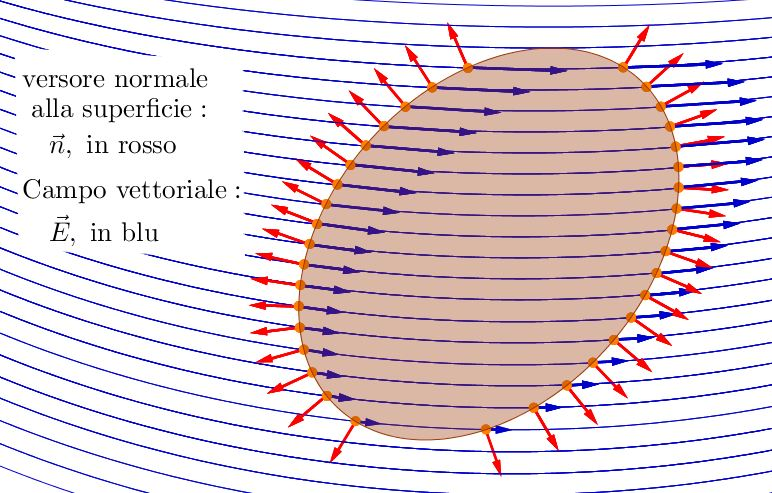
\includegraphics[width=0.6\linewidth]{images/flusso2bis}
	\caption{Schema di una superficie chiusa (da immaginare tridimensionalmente) attraversata da un campo \(\mathbf{E}\).}
	\label{fig:flusso2bis}
\end{figure}
\FloatBarrier
Il flusso è 
\[\Phi(\mathbf{F}) = _S\oint \mathbf{F}d\mathbf{s}\]
dove il simbolo del doppio integrale cerchiato indica l'integrale di superficie chiusa.\\
Se tagliamo la superficie chiusa in due parti \(S_1\) ed \(S_2\), mediante una superficie trasversale G, l'integrale sull'intera superficie, per l'additività dell'integrale, è semplicemente la somma degli integrali di superficie su \(S_1\) ed \(S_2\).
\[\Phi(\mathbf{F}) = _{S_1}\iint \mathbf{F}d\mathbf{s}+_{S_2}\iint \mathbf{F}d\mathbf{s}\]
Possiamo aggiungere e sottrarre l'integrale di superficie aperte su G 
\[\Phi(\mathbf{F}) = _{S_1}\iint \mathbf{F}d\mathbf{s}+_{S_2}\iint \mathbf{F}d\mathbf{s}+_{G}\iint \mathbf{F}d\mathbf{s}-_{G}\iint \mathbf{F}d\mathbf{s}\]
Si noti che avendo diviso la superficie chiusa S in due mediante G, abbiamo ottenuto due nuove superfici chiuse se consideriamo \(S_1^* = S_1+G\) e \(S_2^* = S_2+G\). Il contributo che fornisce G nell'integrale delle due superfici chiuse è uguale in modulo ma di segno opposto, quindi possiamo unire a due a due gli addendi dell'espressione precedente ottenendo due integrali di superficie chiusa (il doppio o triplo integrale chiuso sarà indicato sempre con il simbolo "\(\oint\)")
\[\Phi(\mathbf{F}) = _{S_1^*}\oint \mathbf{F}d\mathbf{s}+_{S_2^*}\oint \mathbf{F}d\mathbf{s}\]
Possiamo reiterare questo processo di divisione n volte ottenendo
\[\Phi(\mathbf{F}) = \sum_{i=1}^{n}\ _{S_i^*}\oint \mathbf{F}d\mathbf{s}\]
Moltiplichiamo e dividiamo per il volume \(V_i\) sotteso dall'i-esima superficie chiusa
\[\Phi(\mathbf{F}) = \sum_{i=1}^{n}\left(\frac{_{S_i^*}\oint \mathbf{F}d\mathbf{s}_i}{V_i}\right)V_i\]
Definiamo la \textbf{divergenza} del campo vettoriale $\mathbf{F}$ 
\[div\mathbf{F} = \frac{_{S_i}\oint \mathbf{F}d\mathbf{s}_i}{V_i}\]
In un campo vettoriale, chiamiamo "pozzo" un punto in cui convergono le linee di campo e "sorgente" uno in cui divergono, . Intuitivamente la divergenza ci offre informazioni su quanto un punto sia "pozzo" o "sorgente". 
\begin{figure}[h!]
	\centering
	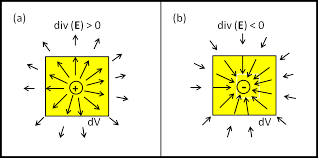
\includegraphics[width=0.6\linewidth]{images/div}
	\caption{Se le linee di campo convergono la divergenza è negativa, se divergono positiva.}
	\label{fig:div}
\end{figure}
\FloatBarrier
Possiamo quindi sostituire e ottenere
\[\Phi(\mathbf{F}) = \sum_{i=1}^{n}div\mathbf{F}V_i\]
Se il numero di divisioni n tende a infinito possiamo passare al continuo 
\[\Phi(\mathbf{F}) = \oint div\mathbf{F}dV\]
quest'ultima relazione è conosciuta come teorema della divergenza o di Gauss. Si noti che la superficie presa in considerazione deve essere chiusa. si noti come in questo teorema mettiamo in relazione il flusso su una superficie con un integrale su un volume, aumentando di 1 la dimensione.\\
\subsubsection{Calcolo della divergenza}
Si consideri un cubo di volume infinitesimo di lati (dx, dy, dz) attraversato da un campo vettoriale $\mathbf{F}(x,y,z) = (F_x, F_y, F_z)$.  
\begin{figure}[h!]
	\centering
	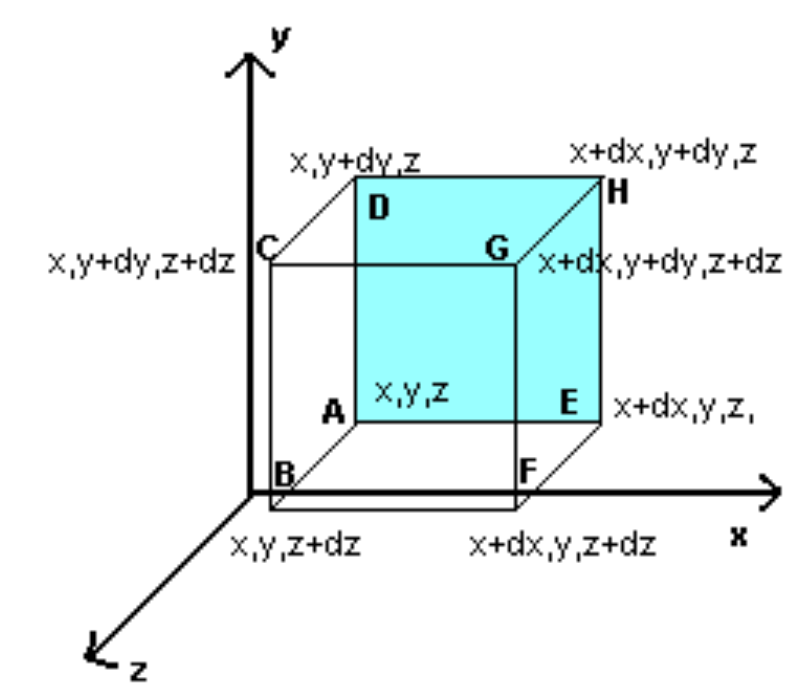
\includegraphics[width=0.6\linewidth]{images/div_quadrato}
	\caption{Schema per il calcolo della divergenza di un campo vettoriale su un cubo.}
	\label{fig:divquadrato}
\end{figure}
\FloatBarrier
La variazione di flusso sull'intero cubo è uguale alla somma dei flusso infinitesimi sulle singole facce. Considerando la faccia "su"
\[d\Phi_{su}(\mathbf{F}) = \mathbf{F}d\mathbf{s}_{su} = \mathbf{F}(x, y, z + dz)dxdy\hat{\mathbf{k}}=F_z(x, y, z + dz)dxdy\]
dove \(F_z\) è la proiezione di sull'asse z ottenuta dal prodotto scalare col versore \(\hat{\mathbf{k}}\). 
Analogamente per la faccia "giù" abbiamo una espressione analoga (in segno meno è dovuto alla convenzione di scegliere il versore normale come uscente dalla superficie chiusa)
\[d\Phi(\mathbf{F}) = -F_z(x, y, z)dxdy\]
Sommando i due flussi infinitesimi otteniamo la variazione infinitesima di flusso sull'asse z
\[d\Phi_z= d\Phi_{su}+d\Phi_{giu}=\left[F_z(x,y,z+dz)-F_z(x,y,z)\right]dxdy=\]
\[\frac{\left[F_z(x,y,z+dz)-F_z(x,y,z)\right]}{dz}dxdydz=\frac{\partial F_z}{\partial z}dxdydz\]
Ripetendo procedimenti analoghi per gli altri assi e sommando otteniamo
\[d\Phi = \left(\frac{\partial F_z}{\partial z}+ \frac{\partial F_z}{\partial z}+ \frac{\partial F_z}{\partial z}\right)dxdydz \]
\[\frac{d\Phi}{dV} = \left(\frac{\partial F_z}{\partial z}+ \frac{\partial F_z}{\partial z}+ \frac{\partial F_z}{\partial z}\right)\]
Ricordando le definizioni di divergenza di $\mathbf{F}$ e di \(\mathbf{\nabla}\) si ottiene
\[div\mathbf{F} = \frac{d\Phi}{dV} = \mathbf{\nabla}\mathbf{F}\]
Si noti che a differenza del gradiente in questo caso il vettore nabla è moltiplicato ad un altro vettore risultando in uno scalare (la divergenza è un operatore scalare definito come il prodotto scalare tra nabla ed un vettore)
\[\Rightarrow \Phi_S(\mathbf{F}) = \iiint \mathbf{\nabla}\mathbf{F}dV = \oint_{V(\Sigma)} \mathbf{\nabla}\mathbf{F}dV\]
che è un'altro modo per esprimere il teorema di Gauss.
\subsection{Teorema di Stokes (teorema del rotore)}
Si consideri la linea chiusa L, fissiamo un verso di percorrenza ed un vettore tangente ad essa $d\mathbf{l}= dl\hat{u}$. 
\begin{definizione}[Circuitazione]
	Definiamo circuitazione infinitesima la quantità
	\[d\Gamma(\mathbf{F}) = \mathbf{F}d\mathbf{l}\]
	La circuitazione è l'integrale di percorso della circuitazione infinitesima
	\[\Gamma(\mathbf{F}) = _L\oint \mathbf{F}d\mathbf{l}\]
\end{definizione}
Analogamente a quanto fatto per la superficie chiusa divisa da una superficie aperta trasversale, possiamo dividere la linea chiusa L mediante una corda G in \(L_1\) ed \(L_2\), e calcolare la circuitazione per le due nuove linee chiuse ottenute \(L_1^* = L_1+G\) e \(L_2^* = L_2+G\).
\[\Gamma_L(\mathbf{F}) = _{L_1^*}\oint \mathbf{F}d\mathbf{l}+_{L_2^*}\oint \mathbf{F}d\mathbf{l} \]
Estendendo il ragionamento ad n divisioni otteniamo
\[\Gamma(\mathbf{F}) = \sum_{i=1}^{n}\ _{L_i}\oint\mathbf{F}d\mathbf{l}\]
Moltiplichiamo e dividiamo per la superficie \(s_i\) sottesa da ciascuna linea chiusa, per trasformarla in vettore, come accennato inizialmente, prendiamo il versore ad essa normale e scegliamo il verso per convenzione usando la regola della mano destra, prendendo come riferimento il verso di percorrenza della linea al contorno.
\[\Gamma(\mathbf{F}) = \sum_{i=1}^{n}\ \left( \frac{_{L_i}\oint\mathbf{F}d\mathbf{l}}{s_i}\right)s_i\]
moltiplichiamo per \(\hat{n}\cdot\hat{n}=1\)
\[\Gamma(\mathbf{F}) = \sum_{i=1}^{n}\ \left( \frac{_{L_i}\oint\mathbf{F}d\mathbf{l}}{s_i}\right)\hat{n}\mathbf{s}_i\]
Definiamo, analogamente a quanto fatto per la divergenza, un nuovo operatore differenziale: il \textbf{rotore}
\[\mathbf{rot}\mathbf{F} = \frac{_{L_i}\oint\mathbf{F}d\mathbf{l}}{s_i}\hat{n}\]
\[\Gamma(\mathbf{F}) = \sum_{i=1}^{n}\mathbf{rot}\mathbf{F}\mathbf{s}_i \]
Se il numero di divisioni tende a infinito passiamo al continuo ottenendo
\[_L\oint\mathbf{F}d\mathbf{l} =\Gamma(\mathbf{F}) = _{S_L}\iint(\mathbf{rot}\mathbf{F})d\mathbf{s}_i =_{S_L}\oint(\mathbf{rot}\mathbf{F})d\mathbf{s}_i\]
Questa relazione è conosciuta come il teorema del rotore o, più frequentemente, come il \textbf{teorema di Stokes}. Si noti come questo metta in relazione un integrale di linea (una dimensione) con un integrale di superficie (due dimensioni).\\\\
In sintesi, per evidenziare un'analogia, i tre teoremi esposti mettono in relazione le dimensioni 0-1 (gradiente), 2-3 (divergenza) ed 1-2 (rotore).
\subsubsection{Calcolo del rotore}
Come per la divergenza, la definizione con cui è stato introdotto il rotore non è operativa: cerchiamo una espressione operativa calcolando la circuitazione di un quadrato infinitesimo ABCD di lati dx e dy scegliendo il senso di percorrenza antiorario. Il quadrato è disposto nello spazio in modo da avere versore coincidente con $\hat{\mathbf{k}}$. 
\begin{align*}
	&\Gamma_L(\mathbf{F}) = _L\oint \mathbf{F} d\mathbf{l} = \int_{A}^{B} \mathbf{F} d\mathbf{l}+\int_{B}^{C} \mathbf{F} d\mathbf{l}+\int_{C}^{D} \mathbf{F} d\mathbf{l}+\int_{D}^{A} \mathbf{F} d\mathbf{l}\\
	&= \int_{x}^{x+dx} F_x(x,y) dx+\int_{y}^{y+dy} F_y(x+dx,y) dy+\int_{x+dx}^{x} F_x(x, y+dy) dx+\int_{y+dy}^{y} F_y(x, y) dy
\end{align*}  
applichiamo quindi il teorema della media integrale che in formule enuncia
\[\int_{A}^{B}f(x)dx=(B-A)f(\overline{x})\]
\[\Rightarrow\Gamma_L(\mathbf{F}) = dxF_x(\overline{x}, y)+dyF_y(x+dx, \overline{y})-dxF_x(\overline{x}, y+dy)-dyF_y(x, \overline{y})\]
\[=-dx[F_x(\overline{x}, y+dy)-F_x(\overline{x}, y)]+dy[F_y(x+dx, \overline{y})-F_y(x, \overline{y})]\]
\[=-dxdy\left[\frac{\partial F_x}{\partial y}\right]+dxdy\left[\frac{\partial F_y}{\partial x}\right] = dxdy\left[\frac{\partial F_y}{\partial x}-\frac{\partial F_x}{\partial y}\right]=\oint\mathbf{F}d\mathbf{l}\]
Ricordando come avevamo definito il rotore, otteniamo 
\[(\mathbf{rot}\mathbf{F})\hat{\mathbf{k}} = \left[\frac{\partial F_y}{\partial x}-\frac{\partial F_x}{\partial y}\right]\]
Per le componenti sugli altri assi il ragionamento è del tutto analogo. Notiamo che le tre componenti del rotore appena ottenute si possono ricavare semplicemente calcolando il determinante di una matrice che sulle righe ha rispettivamente i versori, l'operatore di derivata parziale sui tre assi e le componenti del campo vettoriale. In conclusione
\begin{align*}
&\mathbf{rot}\mathbf{F}=\mathbf{\nabla}\wedge\mathbf{F}=det
\begin{pmatrix}
	\hat{\mathbf{i}}&\hat{\mathbf{j}}&\hat{\mathbf{k}}\\
	\frac{\partial}{\partial x}&\frac{\partial}{\partial y}&\frac{\partial}{\partial z}\\
	F_x&F_y&F_z
\end{pmatrix}=\\
&(\frac{\partial F_z}{\partial y}-\frac{\partial F_y}{\partial z})\hat{\mathbf{i}}
-(\frac{\partial F_z}{\partial x}-\frac{\partial F_x}{\partial z})\hat{\mathbf{j}}
+(\frac{\partial F_y}{\partial x}-\frac{\partial F_x}{\partial y})\hat{\mathbf{k}}
\end{align*}
Si dimostra infine che 
\[div(\mathbf{rot}(\mathbf{F})) =\mathbf{\nabla}(\mathbf{\nabla}\wedge\mathbf{F})=0\]
Le quattro condizioni necessarie e sufficienti (equivalenti) perché un campo si dica conservativo sono
\begin{itemize}
	\item \(\oint \mathbf{F}d\mathbf{l} = 0 \)
	\item \(\mathbf{\nabla}\wedge\mathbf{F} = 0\)
	\item \(\exists\varphi \text{campo scalare} : \mathbf{F}=-\mathbf{\nabla}\varphi\)
	\item \(\varphi(B)-\varphi(A) = -\int_{A}^{B}\mathbf{\nabla}\varphi d\mathbf{l}\ \forall L\)
\end{itemize}
\begin{align*}
\frac{c_1(c_2+c_4)}{c_1+c_2+c_3+c_4}-\frac{c_1c_2}{c_1+c_2}
\end{align*}
\end{document}